\documentclass[12pt]{article}

\usepackage{amsthm}
\usepackage{amssymb}
\usepackage{amsmath}
\usepackage{mathtools}
\usepackage{amsfonts}
\usepackage{graphicx}
\usepackage{algpseudocode}
\usepackage{algorithm}
\usepackage{tikz}
\usepackage{paralist}
\usepackage{circuitikz}
\usepackage{listings}
\input{insbox}
\usetikzlibrary{arrows, automata}

\ctikzset{multipoles/thickness=1.5}
\ctikzset{multipoles/flipflop/width=0.6}
\ctikzset{multipoles/flipflop/pin spacing=0.4}

\tikzset{mux 3by1/.style={muxdemux,muxdemux def={Lh=5, NL=3, NT=1, Rh=3, NB=1, w=2},external pins width=0}}
\tikzset{mux 3by1s/.style={muxdemux,muxdemux def={Lh=3.5, NL=3, Rh=2, NB=1, w=1.5},external pins width=0}}
\tikzset{mux 3by1b/.style={muxdemux,muxdemux def={Lh=6, NL=3,NT=1, Rh=4, NB=1, w=2},external pins width=0}}
\tikzset{carryadder/.style={muxdemux,muxdemux def={Lh=6, NL=2, Rh=3, NR=1, NB=2,NT=2, w=2.5, inset w=0.75, inset Lh=3, inset Rh=2.25},external pins width=0}}
\tikzset{compadder/.style={muxdemux,muxdemux def={Lh=8, NL=2, Rh=4.5, NR=3, NB=2,NT=2, w=2.75, inset w=0.75, inset Lh=4, inset Rh=3},external pins width=0}}
\tikzset{sideFF/.style={flipflop,
flipflop def={t2={\tiny Q}, t5={\tiny D}, cu=1},rotate=90}}

\definecolor{background}{RGB}{39, 40, 34}
\definecolor{string}{RGB}{230, 219, 116}
\definecolor{comment}{RGB}{117, 113, 94}
\definecolor{normal}{RGB}{248, 248, 242}
\definecolor{identifier}{RGB}{50, 50, 250}

\lstdefinestyle{C}{
  language=C,
  numbers=left,
  stepnumber=1,        
  numbersep=5pt,
  numberstyle=\tiny\color{gray}\ttfamily,
  backgroundcolor=\color{white},
  showspaces=false,
  showstringspaces=false,
  showtabs=false,
  tabsize=4,
  captionpos=b,
  breaklines=true,
  breakatwhitespace=true,
  title=\lstname,
  basicstyle=\color{black}\ttfamily,
  keywordstyle=\color{magenta}\ttfamily,
  stringstyle=\color{string}\ttfamily,
  commentstyle=\color{comment}\ttfamily,
  emph={int, char},
  emphstyle=\color{identifier}\ttfamily
}

\lstdefinestyle{DLX}{
  language=[x86masm]Assembler,
  numbers=left,
  stepnumber=1,       
  numbersep=0pt,   
  numberstyle=\tiny\color{gray}\ttfamily,
  backgroundcolor=\color{white},
  showspaces=false,
  showstringspaces=false,
  showtabs=false,
  tabsize=2,
  captionpos=b,
  breaklines=true,
  breakatwhitespace=true,
  framesep=2pt,
  title=\lstname,
  basicstyle=\color{black}\ttfamily,
  stringstyle=\color{string}\ttfamily,
  commentstyle=\color{comment}\ttfamily,
  emph={lw, sw, add, sub, addi, sgti, beqz, bnez, halt},
  emphstyle=\color{purple}\ttfamily
}

\usepackage[
    type={CC},
    modifier={by-nc-sa},
    version={4.0},
]{doclicense}

\title{%
  Digital Logical Systems \\
  \large Notes from TAU Course with Additional Information \\
  Lecturer: Guy Even
}
\author{Gabriel Domingues}
\date{\today}

\let\emptyset\varnothing
\let\RA\Rightarrow
\let\LA\Leftarrow
\let\LR\Leftrightarrow
\let\bar\overline
\let\aand\wedge
\let\oor\vee
\renewcommand{\arraystretch}{0.8}

\newcommand{\set}[2]{\left\{{#1}\;\middle|\;{#2}\right\}}
\newcommand{\Forall}[1]{\forall\,{#1}\,,\,}
\newcommand{\Exist}[1]{\exists\,{#1}:}
\newcommand{\NExist}[1]{\nexists\,{#1}:}
\newcommand{\seq}[2][0]{\left\{{#1},\cdots,{#2}\right\}}
\newcommand{\scr}[1]{{\scriptstyle\textup{#1}}}
\newcommand{\scrf}[1]{{\scriptstyle\textup{\footnotesize #1}}}
\DeclareMathOperator{\N}{\mathbb{N}}
\DeclareMathOperator{\R}{\mathbb{R}}
\DeclareMathOperator{\Ord}{\mathcal{O}}
\DeclareMathOperator{\C}{\mathcal{C}}
\DeclareMathOperator{\Circ}{\mathbb{C}}
\DeclareMathOperator{\BF}{\mathcal{BF}}
\DeclareMathOperator{\fmod}{mod}
\DeclareMathOperator{\id}{id}

\DeclareMathOperator{\NOT}{\scr{NOT}}
\DeclareMathOperator{\OR}{\scr{OR}}
\DeclareMathOperator{\AND}{\scr{AND}}
\DeclareMathOperator{\XOR}{\scr{XOR}}
\DeclareMathOperator{\NOR}{\scr{NOR}}
\DeclareMathOperator{\NAND}{\scr{NAND}}
\DeclareMathOperator{\MUX}{\scr{MUX}}
\DeclareMathOperator{\CLK}{\scr{CLK}}

\newcommand*{\B}{\{0,1\}}
\newcommand{\repr}[1]{\langle{#1}\rangle}
\newcommand{\trepr}[1]{\big[{#1}\big]}
\newcommand{\rto}[1]{\overset{\displaystyle #1}{\longrightarrow}}
\newcommand{\sm}[1]{\setminus\{#1\}}
\newcommand{\floor}[1]{\left\lfloor{#1}\right\rfloor}
\newcommand{\ceil}[1]{\left\lceil{#1}\right\rceil}

\newcommand*{\degin}{\deg_{\text{in}}}
\newcommand*{\degout}{\deg_{\text{out}}}
\DeclareMathOperator{\vars}{vars}
\DeclareMathOperator{\cone}{cone}


\newenvironment{graph}{
\begin{tikzpicture}[
    > = stealth, % arrow head style
    shorten > = 1pt, % don't touch arrow head to node
    auto,
    node distance = 3cm, % distance between nodes
    semithick % line style
  ]
  \tikzstyle{every state}=[
    draw = black,
    thick,
    fill = white,
    minimum size = 4mm
  ]}
{\end{tikzpicture}}

\newtheorem{theorem}{Theorem}[subsection]
\newtheorem{definition}[theorem]{Definition}
\newtheorem{lemma}[theorem]{Lemma}
\newtheorem{corollary}[theorem]{Corollary}
\newtheorem{example}[theorem]{Example}
\newtheorem{remark}[theorem]{Remark}
\newtheorem{design}[theorem]{Design}

\begin{document}
\maketitle

\tableofcontents

\doclicenseThis

\pagebreak

\section{Discrete Mathematics}

\subsection{Set Theory (Succinctly)}

There will be no definition of a set. Instead, we postulate the existence of a relation $\in$ (read as "is in"). 

\begin{definition}[Empty]
  It is axiom the existence of the empty set $\emptyset$, that is, $\Exist{\emptyset}\Forall{x} x\notin\emptyset$
\end{definition}

\begin{definition}[Principle of Double Inclusion]
  We define the following symbols:
  \begin{compactitem}
    \item[] Inclusion: $A\subseteq B\LR \Forall{x} x\in A\RA \;x\in B$
    \item[] Equality: $A=B\LR A\subseteq B$ and $B\subseteq A\LR \Forall{x} x\in A\LR \;x\in B$
    \item[] Proper Inclusion: $A\subsetneq B\LR A\subseteq B$ and $A\neq B$
  \end{compactitem}
\end{definition}

\begin{remark}[Contrapositive]
  \label{contrapositive}
  For two propositions $P$ and $Q$. Then the proposition $P\RA Q$ is equivalent to $\neg Q \RA \neg P$, where $\neg P$ is the oppositive statement.
\end{remark}

\begin{definition}[PRC]
  \label{prc}
  We can create new sets by the Principle of Restricted Comprehension: Let $A$ be a set and $P$ a predicate (given an object, it is either True or False), then the following is a set: $\set{x\in A}{P(x)}$
\end{definition}

\begin{example}[Set Difference]
  Let $A$ and $B$ be any two sets. Construct: $A\setminus B=\set{x\in A}{x\notin B}$ (which is a set cf. \ref{prc})
\end{example}

\begin{definition}[Complement]
  Let $A\subseteq U$. Define $\bar{A}=U\setminus A$.
\end{definition}

\begin{lemma}[Double Complement]
  For any $A\subseteq U$, $\bar{\bar{A}}=A$.
  \begin{proof}
    Double Inclusion:
    \begin{compactitem}
      \item [$(\subseteq)$] For any $x\in U$, $x\in\bar{\bar{A}}\RA x\notin \bar{A}\RA x\in A$
      \item [$(\supseteq)$] For any $x\in U$, $x\notin A\RA x\in \bar{A}\RA x\notin\bar{\bar{A}}$, by contrapositive (cf. \ref{contrapositive}).
    \end{compactitem}
  \end{proof}
\end{lemma}

\begin{definition}[Power Set]
  It is also axiom the existence of the power set: Given a set $A$, there is a set $\mathcal{P}(A)$ so that: $x\in \mathcal{P}(A) \LR x \subseteq A$
\end{definition}

\begin{remark}
  $\Forall{A}\emptyset\in\mathcal{P}(A)$
\end{remark}

\begin{definition}[Set Operations]
  For sets $A$ and $B$ these are sets (by axiom):
  \begin{compactitem}
    \item[] Union : $A\cup B=\set{x}{x\in A \text{ or } x\in B}$
    \item[] Intersection : $A\cap B=\set{x}{x\in A \text{ and } x\in B}$
    \item[] Cartesian Product : $A\times B=\set{(a,b)}{a\in A \text{ and } b\in B}$
  \end{compactitem}
  Note we use Universal Comprehension, but Zermelo-Frankel axioms guarantee those are sets (Axiom of Pairing).
\end{definition}

\begin{example}
  If we define $(a,b):=\{\{a\},\{a,b\}\}$, then the comparision $(a',b')=(a,b)\LR a'=a\text{ and }b'=b$ is imediatelly satisfied. This is a construction that only use the Axiom of Pairing and PRC (cf. \ref{prc}) to build the Cartesian Product.
\end{example}

\begin{definition}[Cartesian Products]
  We define recursively: 
  \begin{compactitem}
    \item[] Base Case: $A^0=\{\emptyset\},\,A^1=A$
    \item[] Reduction: $A^n=A\times A^{n-1}$
  \end{compactitem}
\end{definition}

% \begin{theorem}[DeMorgan's Laws]
%   Let $A,B\subseteq U$. Then: $$\bar{(A\cap B)}=\bar{A}\cup\bar{B}\;\text{ and }\;\bar{(A\cup B)}=\bar{A}\cap\bar{B}$$
%   \begin{proof}
%     We prove each one:
%     \begin{compactenum}
%       \item Double Inclusion:
%       \begin{compactitem}
%         \item [$(\subseteq)$] For any $x\in U$, $x\in\bar{(A\cap B)}\RA x\notin A\cap B\RA x\notin A\text{ or }x\notin B\RA x\in\bar{A}\text{ or }x\in\bar{B}\RA x\in \bar{A}\cup\bar{B}$
%         \item [$(\supseteq)$] For any $x\in U$, $x\notin\bar{(A\cap B)}\RA x\in A\cap B \RA x\in A\text{ and }x\in B\RA x\notin\bar{A}\text{ and }x\notin\bar{B}\RA x\notin \bar{A}\cup\bar{B}$, by contrapositive (cf. \ref{contrapositive}).
%       \end{compactitem}
%       \item We use $\bar{\bar{A}}=A$: $\bar{(A\cup B)}=\bar{\Big(\bar{\bar{A}}\cup \bar{\bar{B}}\Big)}=\bar{\bar{\Big(\bar{A}\cap\bar{B}\Big)}}=\bar{A}\cap\bar{B}$
%     \end{compactenum}
%   \end{proof}
% \end{theorem}

\begin{remark}
  We can construct the sets we will mainly use:
  \begin{compactitem}
    \item [] Bits $\B=\{0,1\}$
    \item [] Natural Numbers $\N=\{0,1,2,\cdots\}$
    \item [] Integer Numbers $\mathbb{Z}=\{\cdots,-2,-1,0,1,2,\cdots\}$
  \end{compactitem}
  Note: $\N$ is formally defined using $0:=\emptyset$, the successor: $\operatorname{Succ}(n)=\{n\}$, so for example, $3:=\{\{\{\emptyset\}\}\}$.
\end{remark}

\begin{definition}[Equivalence Relation]
  \label{equiv_rel}
  An equivalence relation on a set $X$ is a relation, denoted $x \sim y$, that has these three properties:
  \begin{table}[H]
    \centering
    \begin{tabular}{|c|c|}\hline
      Reflexivity & $\Forall{x \in X} x \sim x$\\\hline
      Symmetry & $\Forall{x,y \in X} x \sim y \;  \LR \; y \sim x$ \\\hline
      Transitivity & $\Forall{x,y,z \in X} x \sim y \text{ and } y \sim z \RA x \sim z$\\\hline
    \end{tabular}
  \end{table}
  Further, we define: $[x]=\set{y\in X}{x\sim y}$ and $X/\sim=\set{[x]}{x\in X}$
\end{definition}

\begin{definition}[Binary Relation]
  A subset $R\subseteq A\times B$ is called a relation.
\end{definition}

\begin{example}
  $A=B=\B$, we define $R=\{(0,0),(0,1),(1,0)\}\subseteq A\times B$. Why? Because we can.
\end{example}

\begin{definition}[Function]
  A relation $f\subseteq A\times B$ is called a function iff: $$\Forall{a\in A}\Exist{!\,b\in B}(a,b)\in f$$ Instead of writing $(a,b)\in f$, we write $f(a)=b$. Moreover, $A=D_f$ is called the domain, $B=R_f$ the range and $f\subseteq A\times B$ (sometimes denoted $G_f$) the table/graph. We denote $f:A\to B$.
\end{definition}

\begin{definition}[Composition]
  Let $f:A\to B$ and $g:B\to C$ be two functions (sufficient  $R_f\subseteq D_g$), the composition $g\circ f$ is the function:$$
  \begin{aligned}
    h: A&\to C\\
    a&\mapsto g\big(f(a)\big)
  \end{aligned}$$
\end{definition}

\begin{definition}[Operation]
  An operation $*$ on a set $A$ is a function: $$
  \begin{aligned}
    *: A\times A&\to A\\
    (a,b)&\mapsto a*b
  \end{aligned}$$
  Notice we denote $a*b$ instead of $*(a,b)$. An operation can have (or lack) multiple properties. These are the most important:
  \begin{table}[H]
    \centering
    \renewcommand{\arraystretch}{1.5}
    \begin{tabular}{|c|c|c|}\hline
      Properties & Definition & Structure \\\hline
      Associative & $\Forall{a,b,c\in A} (a*b)*c=a*(b*c)$ & Semigroup\\\hline
      Neutral Element & $\Exist{e\in A}\Forall{a\in A}a*e=e*a=a$ & Monoid\\\hline
      Inverse Element & $\Forall{a\in A}\Exist{b\in A} a*b=b*a=e$ & Group\\\hline
      Commutative & $\Forall{a,b\in A} a*b=b*a$ & Abelian Group\\\hline
    \end{tabular}
  \end{table} 
  \noindent where we named a structure if it has all previous properties. That is, a monoid has an associative operation with identity element.
\end{definition}

\begin{lemma}
  Composition is associative. That is, $f\circ(g\circ h)=(f\circ g)\circ h$.
  \begin{proof} For any $a\in D_f$, $[f\circ(g\circ h)](a)=f([g\circ h](a))=f(g(h(a)))=[f\circ g](h(a))=[(f\circ g)\circ h](a)$. Then, $f\circ(g\circ h)$ and $(f\circ g)\circ h$ are the same function (equality of functions).
  \end{proof}
\end{lemma}

\begin{remark}
  $\mathcal{F}(A)=\set{f\in \mathcal{P}(A\times A)}{f:A\to A}$ is a monoid with composition. The identity is: $\id_A:A\to A$ where $\Forall{a\in A}\id_A(a):=a$.
\end{remark}

\begin{definition}[Restriction and Extension]
  For $f:A\to B$ a function:
  \begin{compactenum}[(a)]
    \item $C\subseteq A$, we define $f|_{C}:C\to B$ as the restriction of $f$ to $C$. Formaly, we write $f|_{C}=\set{(a,b)\in f}{a\in C}=(C\times B)\cap f$. 
    \item $D\supseteq A$, $g:D\to B$ is an extension if $f=g|_A$. Equivalently, $f\subseteq g$.
  \end{compactenum}
\end{definition}

\begin{definition}
  \label{fn_defs}
  A function $f:A\to B$ is:
  \begin{compactitem}
    \item Injective if $\Forall{x,y\in A}f(x)=f(y)\RA x=y$
    \item Surjective if $\Forall{b\in B}\Exist{a\in A}f(a)=b$
    \item Bijective if Injective \& Surjective
  \end{compactitem}
\end{definition}

\begin{lemma}
  \label{inverses}
  A function $f:A\to B$ iff bijective iff $\Exist{g:B\to A}g\circ f=\id_A$ and $f\circ g=\id_B$.
  \begin{proof}
    Observe, by definition $f$ is bijective iff $\Forall{b\in B}\Exist{!\,a\in A}f(a)=b$. Hence, the relation $g=\set{(b,a)\in B\times A}{f(a)=b}$ is a function.
  \end{proof}
\end{lemma}

\begin{definition}[Cardinality]
  We define $\# A=n$ if there is a bijection (cf. \ref{fn_defs}) $\rho:A\to\seq[1]{n}$.
\end{definition}

\begin{remark}
  This definition relies on the fact there another no bijections from $\seq[1]{n}\to\seq[1]{m}$ if $n\neq m$.
\end{remark}

\begin{lemma}
  \label{addition_rule}
  We write $A\sqcup B=A\cup B$ if $A\cap B=\emptyset$. Then: $$\#(A\sqcup B)=\#A+\#B$$ 
  \begin{proof}
    Let $\rho_A:A\to\seq[1]{n}$ and $\rho_B:B\to\seq[1]{m}$ be bijections (for $\#A=n$ and $\#B=m$). Then: $\rho:A\sqcup B\to\seq[1]{n+m}$ defined: $$\rho(c)=\begin{cases}
      \rho_A(c)&\text{ if }c\in A\\
      \rho_B(c)+n&\text{ if }c\in B
    \end{cases}$$
    which is a bijection, since (cf. \ref{inverses}) it has an inverse: $$\rho^{-1}(k)=\begin{cases}
      \rho_A^{-1}(k)&\text{ if }k\leq n\\
      \rho_B^{-1}(k-n)&\text{ if }k>n
    \end{cases}$$
  \end{proof}
\end{lemma}

\pagebreak

\subsection{Recursion and Induction}

\begin{theorem}[Peano Induction]
  Let $P\subseteq \N$. Then, if:
  \begin{compactitem}
    \item Base Case: $0\in P$
    \item Inductive Step: $\Forall{n\in\N} n\in P \RA n+1\in P$
  \end{compactitem}
  Then, $P=\N$. Further, $n\in P$ is called the induction hypothesis.
\end{theorem}

\begin{remark}
  If we want to prove a certain property $P$ is valid for all natural numbers (or after $n_0$), we let $P=\set{n\in\N}{P(n)}$ and use induction.
\end{remark}

\begin{corollary}[Stepped Induction]
  Let $P\subseteq \N$. Then, if:
  \begin{compactitem}
    \item Base Case: $n_0\in P$
    \item Inductive Step: $\Forall{n\in\N} n\in P \RA n+1\in P$
  \end{compactitem}
  Then, $\set{n\in\N}{n\geq n_0}\subseteq P$.
\end{corollary}

\begin{corollary}[Strong Induction]
  Let $P\subseteq \N$. Then, if:
  \begin{compactitem}
    \item Base Case: $0\in P$
    \item Inductive Step: $\Forall{n\in\N} \seq{n}\subseteq P \RA n+1\in P$
  \end{compactitem}
  Then, $P=\N$.
\end{corollary}

\begin{theorem}[Counting]
  Let $f:A\to B$ be a function
  \begin{compactenum}
    \item $f$ is injective $\RA\#A\leq \#B$
    \item $f$ is surjective $\RA \#A\geq \#B$
    \item $f$ is bijective $\RA \#A = \#B$
  \end{compactenum}
  \begin{proof}
    We prove each one by induction on $\# A$
    \begin{compactenum}
      \item \begin{compactitem}
        \item Base Case: $\#A=0$, is true that $0\leq \#B$
        \item Induction Step: Let $\# A=n+1$ and $A=A'\sqcup\{a\}$ for $a\in A$ and $B=B'\sqcup\{f(a)\}$. Then $f\cap (A'\times B')$ is injective, so $\#A'\leq\#B'$, by inductive hypothesis. Hence, $\#A=\#A'+1\leq\#B'+1=\#B$ (cf. \ref{addition_rule}).
      \end{compactitem}
      \item \begin{compactitem}
        \item Base Case: $\#A=0$, is true that $0\geq 0=\#B$, since the empty relation is functional iff the image is empty.
        \item Induction Step: Let $\# A=n+1$ and $A=A'\sqcup\{a\}$ for $a\in A$ and $B=B'\sqcup\{f(a)\}$. Then $f\cap (A'\times B')$ is surjective, so $\#A'\geq\#B'$, by inductive hypothesis. Hence, $\#A=\#A'+1\geq\#B'+1=\#B$ (cf. \ref{addition_rule}).
      \end{compactitem}
      \item $f$ is bijective $\RA \# A \leq \# B$ and $\# A \geq \# B$.
    \end{compactenum}
  \end{proof}
\end{theorem}

\begin{corollary}[Pigeonhole Principle]
  For a function $f:A\to B$, if $\#A>\#B$, then $\Exist{x,y\in A}f(x)=f(y)$ and $x\neq y$ (i.e. $f$ is not injective). 
\end{corollary}

\begin{definition}[Recursion]
  A function $f:\N\to\N$ is called recursive if:
  \begin{compactitem}
    \item Base Cases: $\Forall{k\in\seq{n_0}} f(k)$ is defined.
    \item Reduction Rule: $\Forall{n>n_0} f(n)$ is an expression involving (not necessarily all) $\set{f(n-k)}{k\in\seq{n_0}}$.
  \end{compactitem}
  Further, $f$ is well-defined by given only these propositions.
\end{definition}

\pagebreak

\subsection{Binary Representation}

\begin{theorem}[Modulo and Quotient]
  \label{modulo}
  Let $a,b\in \N$, then, $$\Exist{!\,q,r\in \N} a=q\cdot b+r\text{ and }r<b$$
  We define $r= \fmod(a,b)\in\seq{b-1}$.
  \begin{proof}
    We work by complete induction on $a$.
    \begin{compactitem}
      \item Base Case: $a\in\seq{b-1}:a=b\cdot 0+a$
      \item Inductive Step: $a+1=(a-b+1)+b=(q\cdot b+r)+b=(q+1)\cdot b+r$
    \end{compactitem}
    Essentially, we compute $q=\lfloor\frac{a}{b}\rfloor$ (rounding down). Further, it is also valid for $a\in\mathbb{Z}$.
  \end{proof}
\end{theorem}

\begin{definition}
  Given $n\in\N_{\geq 2}$, we define the following equivalence relation in $\mathbb{Z}$ (cf. \ref{equiv_rel}): $$a\equiv b\mod n\LR \fmod(a,n) = \fmod(b,n)$$
  With $[a]_n=\set{b\in\mathbb{Z}}{a\equiv b\mod n}$, we define addition and multiplication: $$[a]_n+[b]_n=[a+b]_n\;\text{ and }\;[a]_n\cdot[b]_n=[a\cdot b]_n$$
  Which we can check is well-defined (i.e. does not depend on the choice of representative). On the future, we'll just write $a+b\mod n$.
\end{definition}

\begin{definition}[Binary String and Concatenation]
  We define a $n$-bit binary string $\vec{A}=A[0\colon n-1]\in\B^n$. The set of all string is $\B^*=\bigcup_{n\in\N} \B^n$. It is a monoid with concatenation operation: $\circ:\B^*\times \B^*\to \B^*$ such that $\vec{C}=\vec{A}\circ\vec{B}$, then: $$C[i]=\begin{cases}
    A[i]&\text{ if }0\leq i< n\\
    B[i-n]&\text{ if }n\leq i<n+m\\
  \end{cases}$$
  Moreover, $(\B^*,\circ)$ is a monoid.
\end{definition}

\begin{remark}
  There is a bit of ambiguity on writing $A[0:n-1]$ and $A[n-1:0]$.
  \begin{compactitem}
    \item For $A[i:j]$, the LSB (least significant bit) is $A[\min\{i,j\}]$
    \item For $A[j:i]$, the MSB (most significant bit) is $A[\max\{i,j\}]$
  \end{compactitem}
  All binary represention mathematics heretofore we'll use $A[n-1:0]$
\end{remark}

\begin{definition}
  For $A[n-1:0]\in \B^*$, we define the number represented by $\vec{A}$ as: $$\repr{A[n-1:0]}=\sum_{i=0}^{n-1}A[i]\cdot 2^i$$
\end{definition}

\begin{remark}
  $\repr{A[n-1:0]}=\repr{A[k-1:0]}+2^k\cdot\repr{A[n-1:k]}$
\end{remark}

\begin{lemma}
  The mapping $\repr{\,\cdot\,}:\B^n\to\set{x\in\N}{0\leq x\leq 2^n-1}$ is a bijection.
  \begin{proof}
    Let $x\in\N$, use algorithm \ref{BR} or \ref{BR'}.
  \end{proof}
\end{lemma}

\begin{corollary}
  The mapping $\repr{\,\cdot\,}:\B^*\to\N$ is a surjection.
\end{corollary}

\begin{algorithm}[H]
  \caption{BR}
  \begin{algorithmic}
    \Function{$\scrf{BR}$}{$k,x\in\N$}
      \If{$x\geq 2^k$}
        \State\Return Nothing
      \ElsIf{$k=1$}
        \State \Return $x$
      \ElsIf{$x\geq 2^{k-1}$}
        \State \Return $1\circ \scrf{BR}(k-1,x-2^{k-1})$
      \Else
        \State \Return $0\circ \scrf{BR}(k-1,x)$
      \EndIf
    \EndFunction
  \end{algorithmic}
  \label{BR}
\end{algorithm}

\begin{algorithm}[H]
  \caption{BR'}
  \begin{algorithmic}
    \Function{$\scrf{BR}'$}{$k,x\in\N$}
      \If{$x\geq 2^k$}
        \State\Return Nothing
      \ElsIf{$k=1$}
        \State \Return $x$
      \ElsIf{$x$ is even}
        \State \Return $\scrf{BR}'(k-1,x/2)\circ 0$
      \ElsIf{$x$ is odd}
        \State \Return $\scrf{BR}'(k-1,(x-1)/2)\circ 1$
      \EndIf
    \EndFunction
  \end{algorithmic}
  \label{BR'}
\end{algorithm}

\begin{lemma}
  The following are true:
  \begin{compactenum}[(i)]
    \item $0\leq \repr{A[n-1:0]}\leq 2^n-1$
    \item If $\repr{A[n-1:0]}=\repr{B[m-1:0]}$ with $m\geq n$, then $B=0^{m-n}\circ A$.
  \end{compactenum}
  \begin{proof}
    We prove:
    \begin{compactenum}[(i)]
      \item $0=\sum_{i=0}^{n-1}0\cdot 2^i\leq \sum_{i=0}^{n-1}A[i]\cdot 2^i \leq \sum_{i=0}^{n-1}1\cdot 2^i= 2^n-1$
      \item By definition: $\repr{A[n-1:0]}=\repr{B[n-1:0]}+2^n\cdot\repr{B[m-1:n]}\RA 2^n\cdot\repr{B[m-1:n]}\leq 2^n-1\RA \repr{B[m-1:n]}=0\RA B[m-1:n]=0^{m-n}$
    \end{compactenum}
  \end{proof}
\end{lemma}

\begin{definition}[Two's Complement]
  For $A[n-1:0]\in \B^*$, we define the number represented by $\vec{A}$ in two's complement as: $$\trepr{A[n-1:0]}=-2^{n-1}\cdot A[n-1]+\repr{A[n-2:0]}$$
\end{definition}

\begin{algorithm}[H]
  \caption{TCR}
  \begin{algorithmic}
    \Function{$\scrf{TCR}$}{$n,x\in\N$}
      \If{$x\geq 2^{n-1}\oor x\leq -2^{n-1}-1$}
        \State\Return Nothing
      \ElsIf{$x\geq 0$}
        \State \Return $0\circ\scrf{BR}(n-1,x)$
      \ElsIf{$x<0$}
        \State \Return $\scrf{BR}(n,x+2^n)$
      \EndIf
    \EndFunction
  \end{algorithmic}
  \label{BR'}
\end{algorithm}

\begin{lemma}
  \label{twos_inv}
  The following are true:
  \begin{compactenum}[(i)]
    \item $-2^{n-1}\leq \trepr{A[n-1:0]}\leq 2^{n-1}-1$
    \item $-\trepr{A[n-1:0]}=\trepr{\scr{INV}(A[n-1:0])}+1$
  \end{compactenum}
  \begin{proof}
    We prove:
    \begin{compactenum}[(i)]
      \item $-2^{n-1}+0\leq -2^{n-1}\cdot A[n-1]+\repr{A[n-2:0]} \leq 0+2^{n-1}-1$
      \item $\trepr{A[n-1:0]}+\trepr{\scr{INV}(A[n-1:0])}=-\big(A[n-1]+\scr{INV}(A[n-1])\big)\,2^{n-1}+\sum_{i=0}^{n-2}\big(A[i]+\scr{INV}(A[i])\big)\cdot 2^i=-2^{n-1}+\sum_{i=0}^{n-2}2^i=1$
    \end{compactenum}
  \end{proof}
\end{lemma}

\begin{lemma}[Sign Extension]
  \label{sext}
  The following are true:
  \begin{compactenum}[(i)]
    \item $\trepr{A[n-1:0]}<0\LR A[n-1]=1$
    \item $A[n]=A[n-1]\RA\trepr{A[n:0]}=\trepr{A[n-1:0]}$
  \end{compactenum}
  \begin{proof}
    We prove:
    \begin{compactenum}[(i)]
      \item $A[n-1]=0\RA\trepr{A[n-1:0]}=\repr{A[n-2:0]}\geq 0$ and $A[n-1]\RA-\trepr{A[n-1:0]}=\trepr{\scr{INV}(A[n-1:0])}+1\geq 1\RA \trepr{A[n-1:0]}\leq -1$.
      \item $\trepr{A[n:0]}=-A[n]\cdot 2^n+A[n-1]\cdot 2^{n-1}+\repr{A[n-1:0]}=-A[n-1]\cdot 2^{n-1}+\repr{A[n-1:0]}=\trepr{A[n-1:0]}$
    \end{compactenum}
  \end{proof}
\end{lemma}

\begin{corollary}
  $\trepr{A[n-1]^k\circ A[n-1:0]}=\trepr{A[n-1:0]}$ we denote the sign extension to $n+k$ bits: $\text{sext}_{n+k}(A[n-1:0]):=A[n-1]^k\circ A[n-1:0]$.
\end{corollary}

\pagebreak

\subsection{Graph Theory}

\begin{definition}[Directed Graph]
  Let $V$ be a finite set and $E\subseteq V\times V$. The pair $G=(V,E)$ is called a directed graph. We say $v\in V$ is a vertex/node and $e=(u,v)\in E$ is an (directed) edge.
\end{definition}

\begin{example} The set $V=\{0,1,2,3,4\}$ and $$E=\{(0,1),(0,2),(0,3),(1,4),(1,1),(2,1),(2,3),(3,2)\}$$ which we can draw as follows:
  \begin{figure}[ht!]\centering
    \begin{graph}
      \node[state] (v0) {$v_0$};
      \node[state] (v1) [above right of=v0] {$v_1$};
      \node[state] (v2) [right of=v0] {$v_2$};
      \node[state] (v3) [below right of=v0] {$v_3$};
      \node[state] (v4) [right of=v2] {$v_4$};
      \path[->]
      (v0)  edge node {$e_0$} (v1)
            edge node {$e_1$} (v2)
            edge node {$e_2$} (v3);
      \path[->]
      (v1)  edge node {$e_3$} (v4)
            edge[loop above] node {$e_4$} (v1);
      \path[->]
      (v2)  edge node {$e_5$} (v1)
            edge[bend left] node {$e_6$} (v3);
      \path[->] 
      (v3)  edge node {$e_7$} (v2);
    \end{graph}
  \end{figure}
  
  \noindent Notice we allow for self-loops like $(1,1)$ and 2-cycles like $(2,3)$ and $(3,2)$, but we do not allow repeated edges. 
\end{example}

\begin{definition}[Subgraph]
  \label{def_induced}
  For $G=(V,E)$ a graph, let $U\subseteq V$, we denote $G[U]=(U,\set{(u,v)\in E}{u,v\in U})$ the induced subgraph.
\end{definition}

\begin{definition}[Path]
  A path of length $\ell$ (that is, $\ell=\#\Gamma$) in $G=(V,E)$ is a pair $\Gamma\in V^{\ell+1}$ such that $\Forall{i\in\seq{\ell-1}} (v_i,v_{i+1})\in E$. We denote $\Gamma$ by: $v_0\rto{e_0}v_1\rto{e_1}v_2\cdots v_{\ell-1}\rto{e_{\ell-1}}v_\ell\text{ or }v_0\rto{\Gamma} v_\ell$
\end{definition}

\begin{remark}
  \label{null_path}
  There is always a path of length $1$ from $v$ to $v$, $\Gamma=(v,\emptyset)$.
\end{remark}

\begin{definition}[Closed and Simple Paths]
  A path is closed (called a cycle) if $v_0=v_\ell$ and is open otherwise. An open path is simple if every element of $\mathcal{V}$ are distinct. Likewise, a cycle is simple if every element of $\mathcal{V}\setminus(v_\ell)$ are distinct.
\end{definition}

\begin{lemma}
  A non-simple path contains a cycle.
  \begin{proof}
    If $\Gamma$ is a cycle, we are done. Else, if $\Gamma$ is open and non-simple, let $v_i=v_j\in\mathcal{V}$. Then, $v_i\rto{\Gamma}v_j=v_i$ is a cycle.
  \end{proof}
\end{lemma}

\begin{definition}[DAG]
  A directed acyclic graph (DAG) is a directed graph that has no cycles.
\end{definition}

\begin{corollary}
  Every path in a DAG is simple.
\end{corollary}

\begin{definition}[Degrees, Sources and Sinks]
  Given a graph $G=(V,E)$ and $v\in V$, we define:
  \begin{align*}
    \degin(v)&=\#\set{e\in E}{\Exist{u\in V} e=(u,v)}\\
    \degout(v)&=\#\set{e\in E}{\Exist{u\in V} e=(v,u)}
  \end{align*}
  Further, if $\degin(v)=0$, $v$ is called a \textbf{source}. If $\degout(v)=0$, $v$ is called a \textbf{sink}.
\end{definition}

\begin{theorem}
  \label{dag_sink}
  Every DAG has at least one sink.
  \begin{proof}
    By contrary, suppose $G$ has no sink, that is, $\Forall{v\in V} \degout(v)>0$. Take $v_0\in V$. Since $\degin(v_0)>1$, take $v_1\in V:e_0=(v_0,v_1)\in E$. We can continue to create a path $v_0\rto{\Gamma}v_\ell$ of arbitrary length. If $\Gamma$ is simple, take $\ell=\#V$, hence, the path has more vertices than there are in $V$, contradiction. If $\Gamma$ is not simple, then $G$ has a cycle, contradiction.
  \end{proof}
\end{theorem}

\begin{corollary}
  Every DAG has at least one source.
  \begin{proof}
    Take $G'=(V,E')$ where $$E'=\set{(v,u)\in V\times V}{(u,v)\in E}$$ the reversed graph. Notice $G'$ is also acylic, since a cycle in $G'$ implies a cycle in $G$ with the edges and the order reversed. By the theorem, there is a sink $u$. Since $\Forall{v\in V}\degin'(v)=\degout(v)$, we get: $\degout(u)=\degin'(u)=0$.
  \end{proof}
\end{corollary}

\begin{lemma}
  \label{induced_DAG}
  An induced subgraph (cf. \ref{def_induced}) of a DAG is still a DAG.
  \begin{proof}
    If there is a cycle in $G[U]$, then the same cycle exists in $G$, since $U\subseteq V$ and $E_U\subseteq E$. Hence, $G[U]$ has no cycles.
  \end{proof}
\end{lemma}

\begin{definition}[Topological Ordering]
  Let $G=(V,E)$ be a graph. A topological ordering is map $\pi:V\to\seq{\#V-1}$ such that:
  $$\Forall{u,v\in V}(u,v)\in E\RA \pi(u)<\pi(v)$$
\end{definition}

\begin{remark}[Topological Sorting]
  Since $\pi:V\to\seq{\#V-1}$ is a bijection, we can write $V=(v_0,v_1,\cdots,v_{\#V-1})$ where $v_i=\pi^{-1}(i)$.
\end{remark}

\begin{algorithm}[H]
  \caption{Kahn's Algorithm}
  \begin{algorithmic}
    \Function{$\scrf{TO}$}{$G=(V,E)$}
      \If{$\#V=1$}
        \State \Return $\pi(v_0)=0$
      \Else
        \State $s \gets \scrf{sink}(V,E)$
        \State \Return $\scrf{TO}(G[V\sm{s}])$ with $\pi(s)=\#V-1$
      \EndIf
    \EndFunction
  \end{algorithmic}
  \label{Kahn}
\end{algorithm}

\begin{theorem}
  A graph is a DAG iff it has a topological ordering.
  \begin{proof}
    We prove both directions:
    \begin{compactitem}
      \item[$(\LA)$] Suppose $G$ has a topological ordering $\pi$. Take a path $\Gamma:v_0\rto{e_0}v_1\rto{e_1}v_2\cdots v_{\ell-1}\rto{e_{\ell-1}}v_\ell$, then $\pi(v_0)<\pi(v_1)<\cdots<\pi(v_{\ell-1})<\pi(v_\ell)$. Hence, for any path $\pi(v_0)\neq\pi(v_\ell)$, so $G$ has no cycles.
      \item[$(\RA)$] We'll prove that algorithm \ref{Kahn} produces a topological ordering by induction. The base case is true by construction of the function. Let $\#V=n+1$. Now, suppose $\scrf{TO}(G[V\sm{s}])$ is a topological ordering $\pi: V\sm{s}\to\seq{n-1}$, where $s=\scrf{sink}(V,E)$, which exists by theorem. Since $\pi$ is a bijection, extending to $\pi(s)=\#V-1=n$ is still a bijection. Notice if $(v,s)\in E\RA v\neq s\RA \pi(v)<\pi(s)=n$, further, $\NExist{v\in V}(s,v)\in E$, since $s$ is a source. Therefore, since $\pi$ is already a topological ordering of $G[V\sm{s}]$, the extension is also a topological ordering.
    \end{compactitem}
  \end{proof}
\end{theorem}

\begin{remark}
  Observe that algorithm \ref{Kahn} relies on the fact that there is a sink in $G$ (cf. \ref{dag_sink}) and that the induced subgraph is also a DAG (cf. \ref{induced_DAG}).
\end{remark}

\begin{example}
  The following is the result after applying the algorithm:
  \begin{figure}[H]
    \centering
    \begin{minipage}{0.45\linewidth}
      \centering
      \begin{graph}
        \node[state] (v0) {$v_0$};
        \node[state] (v1) [below right of=v0] {$v_1$};
        \node[state] (v2) [right of=v0] {$v_2$};
        \node[state] (v3) [above right of=v0] {$v_3$};
        \node[state] (v4) [left of=v1] {$v_4$};
        \path[->]
        (v0)  edge node {$e_0$} (v1)
              edge node {$e_1$} (v2)
              edge node {$e_2$} (v3);
        \path[->]
        (v1)  edge node {$e_3$} (v4);
        \path[->]
        (v2)  edge node {$e_4$} (v1);
        \path[->] 
        (v3)  edge node {$e_5$} (v2);
      \end{graph}
    \end{minipage}
    \begin{minipage}{0.45\linewidth}
      \centering
      \begin{tabular}{c|c}
        $v$ & $\pi(v)$\\\hline
        $v_0$ & $0$\\
        $v_1$ & $3$\\
        $v_2$ & $2$\\
        $v_3$ & $1$\\
        $v_4$ & $4$
      \end{tabular}
    \end{minipage}
  \end{figure}
\end{example}

\begin{definition}[Longest Path]
  A path $\Gamma$ is a \textit{longest} path of $G$ if $$\Forall{\Gamma'\text{ path in }G}\#\Gamma'\leq \#\Gamma$$
\end{definition}

\begin{theorem}
  \label{long_path_existence}
  If $G=(V, E)$ is a DAG, then $\Forall{v\in V}$ there is some longest path that ends in $v$. Further, there exists some longest path in $G$.
  \begin{proof}
    Since any path of length bigger than $\#V$ is not simple (which $G$ does not have), we get: $$\Forall{\Gamma\text{ path in }G}\#\Gamma\leq \#V-1$$ Since there are a finite number of paths end in $v\in V$, there must be some biggest element. The same argument follows for any path in $G$.
  \end{proof}
\end{theorem}

\begin{definition}[Delay Function]
  \label{def_delay}
  Given $G=(V,E)$ a DAG, we define $d:V\to\N$, so that $\Forall{v\in V} d(v)=$ \emph{length of longest path ending in $v$}, which exist cf. \ref{long_path_existence}.
\end{definition}

\begin{algorithm}[H]
  \caption{Longest Path Algorithm}
  \begin{algorithmic}
    \State $(v_0,\cdots,v_{n-1})\gets \scrf{TS}(V,E)$
    \For{$0\leq j\leq n-1$}
      \If{$v_j$ is a source}
        \State $d(v_j)\gets 0$
      \Else
        \State $d(v_j)\gets 1+\max\set{d(v_i)}{i<j\text{ and }(v_i,v_j)\in E}$
      \EndIf
    \EndFor
  \end{algorithmic}
  \label{Longest Path}
\end{algorithm}

\begin{theorem}
  The algorithm \ref{Longest Path} produces the delay function, as in \ref{def_delay}.
  \begin{proof}
    We prove by induction on $j$. By topological sorting, $v_0$ is a source, so $d(v_0)=0$. Suppose $\Forall{i\in\N:0 \leq i\leq j} d(v_i)=$ length of longest path ending in $v_i$. We'll prove the inductive step. If $v_{j+1}$ is a source, we are done. Else, there are $v_i$ such that $(v_i,v_j)\in E$. Since they are sorted, $\Forall{i\in\N:(v_i,v_j)\in E} 0\leq i\leq j$, so the longest path that ends in $v_{j+1}$ must pass through some $v_i$ for $0\leq i\leq j$, and we know how to calculate each delay $d(v_i)$ (by hypothesis). Therefore, $1+\max\set{d(v_i)}{i\leq j\text{ and }(v_i,v_j)\in E}$ computes the desired delay of $v_{j+1}$.
  \end{proof}
\end{theorem}

\begin{definition}[Rooted Tree]
  \label{def_rooted}
  A rooted tree $G=(V,E)$ is a DAG s.t.:
  \begin{enumerate}
    \item There only one sink $r$ in $G$
    \item $\Forall{v\in V\sm{r}} \degout(v)=1$
  \end{enumerate}
  We call the sink $r=r(G)$ the root of $G$.
\end{definition}

\begin{example} $V=\{0,1,2,3,4,5\},E=\{(1, 0), (2, 0), (3, 1), (4, 1), (5, 2)\}$ such that $r=0$:
  \begin{figure}[ht!]\centering
    \begin{graph}
      \node[state] (v0) {$v_0$};
      \node[state] (v1) [below left of=v0] {$v_1$};
      \node[state] (v2) [below right of=v0] {$v_2$};
      \node[state] (v3) [below left of=v1] {$v_3$};
      \node[state] (v4) [below right of=v1] {$v_4$};
      \node[state] (v5) [below right of=v2] {$v_5$};
      \path[->]
      (v1)  edge node {$e_0$} (v0);
      \path[->]
      (v2)  edge node {$e_1$} (v0);
      \path[->]
      (v3)  edge node {$e_2$} (v1);
      \path[->] 
      (v4)  edge node {$e_3$} (v1);
      \path[->]
      (v5)  edge node {$e_4$} (v2);
    \end{graph}
  \end{figure}
\end{example}

\begin{lemma}
  If $G$ is a rooted tree, $\#E=\#V-1$.
  \begin{proof}
    We shall do induction on $\#V$. The base case is $\#V=1$, so $\#E=0$. For the step, suppose any rooted tree with $n$ vertices has $n-1$ edges. Take a rooted tree $G$ with $\#V=n+1$ and a source $s$ of $G$. Since $\degin(s)=0$ and $\degout(s)=1$, there is only on edge in $E$ that contains $s$. Hence, since $G[V\sm{v}]$ is a rooted tree with with $n$ vertices (because we only removed one edge and one vertex), it has $n-1$ edges. Therefore $G$ has $n$ edges.
  \end{proof}
\end{lemma}

\begin{theorem}
  \label{root_unique_path}
  In a rooted tree $G=(V,E)$, for every vertex $v\in V$, there exists an unique path from $v$ to $r(G)$.
  \begin{proof}
    The case $v=r$ is trivial. To prove there must exist a path for any $v\in V\sm{r}$, we take a path $v=v_0\rto{\Gamma}v_\ell$ of arbitrary length $\ell$. If $v_\ell$ is a sink, we are done since $v_\ell=r$. If $v_\ell$ is not a sink, by the definition of a rooted tree, there is a vertex $v_{\ell+1}$ such that $(v_\ell,v_{\ell+1})\in E$, so that $\degout(v)=1$. Therefore, we can continue extending the path. Take $\ell=\# V-1$ at the limiting case, the path has all the vertices, so $v_\ell=r$. To prove uniqueness, if we take two paths $v=v_0\rto{\Gamma}v_\ell=r$ and $v=u_0\rto{\Gamma'}u_\ell=r$. By definition, $\Forall{v\in V\sm{r}}\degout(v)=1$, so $v_1=u_1,\,v_2=u_2,\cdots,\, v_\ell=u_\ell\RA \Gamma=\Gamma'$.
  \end{proof}
\end{theorem}

\begin{definition}
  \label{def_hanging}
  Let $\{r_i\}_{i=1}^k=\set{r_i\in V}{(r_i,r)\in E}$, where $k=\degin(r)$. Define:
  $$V_i=\set{v\in V}{\Exist{\Gamma\text{ path in }G}v\rto{\Gamma}r_i}$$
  and $G_i=(V_i,E_i)=G[V_i]$.
\end{definition}

\begin{remark}
  $r_i\in V_i$ (cf. \ref{null_path})
\end{remark}

\begin{lemma}
  For $G=(V,E)$ a rooted tree:
  \begin{compactenum}
    \item $V=\{r\}\sqcup\big(\bigsqcup_{i=1}^k V_i\big)$
    \item The graph $G_i$ is a rooted tree with $r(G_i)=r_i$ for every $1\leq i\leq k$
  \end{compactenum}
  \begin{proof}
    We prove each one:
    \begin{compactenum}
      \item For $i\neq j$, if $\exists\,v\in V_i\cap V_j$, then there are two different paths from $v$ to $r$: $v\rto{\Gamma}r_i\rto{e_i}r$ and $v\rto{\Gamma'}r_j\rto{e_j}r$. Contradiction (cf. \ref{root_unique_path}). Further since $\Forall{v\in V\sm{r}}$ there is a path to $r$, that path must go through one of the $r_i$. Hence, $v\in V\RA v\in V_i$ for some $i$ or $v=r$.
      \item We need to prove the only sink is $r_i$, since $G_i$ is a DAG (cf. \ref{induced_DAG}). Now, $r_i$ is a sink, since it's only out-edge was $(r_i,r)\notin E_i$. Further, by definition, $\Forall{v\in V\sm{r_i}}\degout(v)>0$, so $r_i$ is the only sink.
    \end{compactenum}
  \end{proof}
\end{lemma}

\begin{definition}[Leaf]
  \label{def_leaf}
  In a rooted tree, a source is called a leaf. Any other vertice is called an interior vertex.
\end{definition}

\pagebreak

\subsection{Asymptotics}

\begin{definition}
  \label{def_order}
  For $f:\N\to\R_{\geq 0}$ and $g:\N\to\R_{\geq 0}$, define the following notation (symbolic equality):
  \begin{compactenum}[(i)]
    \item $f(n)=\Ord(g(n))\LR\Exist{A\in\R_{>0},N\in\N}\Forall{n\geq N}f(n)\leq A\cdot g(n)$
    \item $f(n)=\Omega(g(n))\LR\Exist{A\in\R_{>0},N\in\N}\Forall{n\geq N}f(n)\geq A\cdot g(n)$
    \item $f(n)=\Theta(g(n))\LR f(n)=\Ord(g(n))\text{ and }f(n)=\Omega(g(n))$
  \end{compactenum}
  The intuition is:
  \begin{compactenum}[(i)]
    \item $f(n)=\Ord(g(n)):$ $f$ does not grow faster than $g$ 
    \item $f(n)=\Omega(g(n)):$ $f$ grows at least as fast as $g$ 
    \item $f(n)=\Theta(g(n)):$ $f$ grows as fast as $g$ 
  \end{compactenum}
\end{definition}

\begin{remark}
  The functions $f$ and $g$ may not be defined for finite number of natural and the definition should still work.
\end{remark}

\begin{lemma}
  $f:\N\to\R_{\geq 0}$ and $g:\N\to\R_{\geq 0 }:$
  $$g(n)=\Omega(f(n))\LR f(n)=\Ord(g(n))$$
  \begin{proof}
    By definition (cf. \ref{def_order}), $f(n)\geq A\cdot g(n)\LR g(n)\leq \frac{1}{A}\cdot f(n)$, the result follows.
  \end{proof}
\end{lemma}

\begin{corollary}
  $g(n)=\Theta(f(n))\LR f(n)=\Theta(g(n))$
\end{corollary}

\begin{lemma}
  For $f:\N\to\R_{\geq 0}$ and $g:\N\to\R_{\geq 0}$:
  \begin{compactenum}[(i)]
    \item $f(n)=\Ord(g(n))\RA\Exist{A\in\R_{>0},B\in\R_{\geq 0}}\Forall{n\in\N}f(n)\leq A\cdot g(n)+B$
    \item $f(n)=\Omega(g(n))\LR\Exist{A\in\R_{>0},B\in\R_{\geq 0}}\Forall{n\in\N}f(n)\geq A\cdot g(n)+B$
  \end{compactenum}
  Moreover, if $\Forall{n\in\N}g(n)\geq 1$, the converse of (i) is true.
  \begin{proof}
    We prove:
    \begin{compactenum}[(i)]
      \item $f(n)=\Ord(g(n))\LR\Exist{A\in\R_{>0},N\in\N}\Forall{n\geq N}f(n)\leq A\cdot g(n)\RA$ define $B=\max\set{f(n)}{0\leq n<N}$, so $\Forall{n\in\N}f(n)\leq A\cdot g(n)+B$
      \item $f(n)=\Omega(g(n))\LR\Exist{A\in\R_{>0},N\in\N}\Forall{n\geq N}f(n)\geq A\cdot g(n)\RA$ define $B=\min\Big\{A,\min\set{\frac{f(n)}{g(n)}}{0\leq n<N\text{ and }g(n)\neq 0}\Big\}$, so that we have: $\Forall{n\in\N}f(n)\geq B\cdot g(n)$
    \end{compactenum}
    The converse is given by:
    \begin{compactenum}[(i)]
      \item $f(n)\leq A\cdot g(n)+B\leq (A+B)\cdot g(n)\RA f(n)=\Ord(g(n))$ (supposing $g(n)\geq 1$)
      \item $f(n)\geq A\cdot g(n)+B\geq A\cdot g(n)\RA f(n)=\Omega(g(n))$
    \end{compactenum}
  \end{proof}
\end{lemma}

\begin{theorem}
  Let $f$ and $g$ be both monotonically non-decreasing. Then if $\Exist{\rho\in\R_{>0}}\Forall{k\in\N}$
  \begin{compactenum}[(i)]
    \item $\rho\geq\dfrac{g(2^{k+1})}{g(2^k)}\RA [f(2^k)=\Ord(g(2^k))\RA f(n)=\Ord(g(n))]$
    \item $\rho\leq\dfrac{g(2^{k+1})}{g(2^k)}\RA [f(2^k)=\Omega(g(2^k))\RA f(n)=\Omega(g(n))]$
  \end{compactenum}
  Moreover, if $\dfrac{g(2^{k+1})}{g(2^k)}$ is bounded, then $[f(2^k)=\Theta(g(2^k))\RA f(n)=\Theta(g(n))]$.
  \begin{proof}
    Suppose 
    \begin{compactenum}[(i)]
      \item $f(2^k)=\Ord(g(2^k))\LR\Exist{A\in\R_{>0},K\in\N}\Forall{k\geq K}f(2^k)\leq A\cdot g(2^k)$. For $n\geq 2^K$, $2^k\leq n<2^{k+1}$ for some $k\geq K$. Since $f$ and $g$ are monotonically non-decreasing: $$f(n)\leq f(2^{k+1})\leq A\cdot g(2^{k+1})\leq \rho\cdot A\cdot g(2^k)\leq \rho\cdot A\cdot g(n)$$ Hence, $\Forall{n\geq 2^K}f(n)\leq \rho\cdot A\cdot g(n)$, so, $f(n)=\Ord(g(n))$.
      \item $f(2^k)=\Omega(g(2^k))\LR\Exist{A\in\R_{>0},K\in\N}\Forall{k\geq K}f(2^k)\geq A\cdot g(2^k)$. For $n\geq 2^K$, $2^k\leq n<2^{k+1}$ for some $k\geq K$. Since $f$ and $g$ are monotonically non-decreasing: $$f(n)\geq f(2^k)\geq A\cdot g(2^k)\geq \frac{A}{\rho}\cdot g(2^{k+1})\geq \frac{A}{\rho}\cdot g(n)$$ Hence, $\Forall{n\geq 2^K}f(n)\geq \dfrac{A}{\rho}\cdot g(n)$, so, $f(n)=\Omega(g(n))$.
    \end{compactenum}
    If $\dfrac{g(2^{k+1})}{g(2^k)}$ is bounded, both conditions apply.
  \end{proof}
\end{theorem}

\pagebreak 

\section{Boolean Logic}

\subsection{Prepositional Logic}

\begin{definition}[Boolean Functions]
  A function $B:\B^n\to \B^k$, is called a Boolean function.
\end{definition}

\begin{definition}[Four Basis Boolean Functions]
  \label{boolean_fns}
  Define:
  \begin{table}[H]
    \centering
    \begin{tabular}{cccc}
      \begin{tabular}{c||c}
          $x$ & $\NOT(x)$\\\hline
          $0$ & $1$\\
          $1$ & $0$
      \end{tabular}
      &
      \begin{tabular}{c|c||c}
        $x$ & $y$ & $\AND(x,y)$\\\hline
        $0$ & $0$ & $0$\\
        $0$ & $1$ & $0$\\
        $1$ & $0$ & $0$\\
        $1$ & $1$ & $1$
      \end{tabular}
      &
      \begin{tabular}{c|c||c}
        $x$ & $y$ & $\OR(x,y)$\\\hline
        $0$ & $0$ & $0$\\
        $0$ & $1$ & $1$\\
        $1$ & $0$ & $1$\\
        $1$ & $1$ & $1$
      \end{tabular}
      &
      \begin{tabular}{c|c||c}
        $x$ & $y$ & $\XOR(x,y)$\\\hline
        $0$ & $0$ & $0$\\
        $0$ & $1$ & $1$\\
        $1$ & $0$ & $1$\\
        $1$ & $1$ & $0$
      \end{tabular}
    \end{tabular}
  \end{table}

  \noindent With that, we can define $\NAND=\NOT\circ\AND,\,\NOR=\NOT\circ\OR,\,\scr{XNOR}=\NOT\circ\XOR$. Further, we write the operations:
  \begin{compactitem}
    \item[] Negation: $\neg x:=\NOT(x)$
    \item[] Conjunction: $x\aand y:=\AND(x,y)$
    \item[] Disjunction: $x\oor y:=\OR(x,y)$
  \end{compactitem}
\end{definition}

\begin{lemma}
  \label{bool_identity}
  $\Forall{x\in\B}$
  \begin{compactitem}
    \item $x\aand 1 = x$
    \item $x\aand 0 = 0$
    \item $x\oor 1 = 1$
    \item $x\oor 0 = x$
  \end{compactitem}
  \begin{proof}
    Follows directly from the definition, looking at the truth tables.
  \end{proof}
\end{lemma}

\begin{lemma}[Boolean Monoids]
  We have:
  \begin{compactitem}
    \item[] All: $(\B,\aand)$ is a monoid with identity $1$
    \item[] Any: $(\B,\oor)$ is a monoid with identity $0$
  \end{compactitem}
  \begin{proof}
    For associativity, observe $x\aand(y\aand z)=(x\aand y)\aand z=1\LR x=y=z=1$ and $x\oor(y\oor z)=(x\oor y)\oor z=0 \LR x=y=z=0$. Hence, the truth tables are the same. For the identities, we use the relation in \ref{bool_identity}.
  \end{proof}
\end{lemma}

\begin{definition}
  \label{associative_bools}
  Since the formulas are associate, we define:
  \begin{compactitem}
    \item $\AND_n(x_1,\cdots,x_n)=\AND(\AND_{n-1}(x_1,\cdots,x_{n-1}),x_n)=x_1\aand\cdots\aand x_n$
    \item $\OR_n(x_1,\cdots,x_n)=\OR(\OR_{n-1}(x_1,\cdots,x_{n-1}),x_n)=x_1\oor\cdots\oor x_n$
  \end{compactitem}
\end{definition}

\begin{definition}[Boolean Connectives]
  A boolean formula has a set $U$ of variables and a set $\C$ of connectives. A connective is an operation to build larger formulas. The arity of the connective is the number of arguments it receives.
\end{definition}

\begin{remark}
  Every connective $\gamma$ is exacty one boolean function $B_\gamma:\B^k\to\B$. There is only one (non-trivial) unary connective $\NOT$ (cf. \ref{boolean_fns}), also denoted $\neg$. Further there a many binary connectives, e.g. $\AND$ (denoted $\aand$), $\OR$ (denoted $\oor$), material implication ($\to$) etc.
\end{remark}

\begin{definition}[Parse Tree]
  \label{parse_tree}
  A parse tree is a pair $(G,\pi)$ where $G=(V,E)$ is a rooted tree and $\pi:V\to\B\cup\,U\cup\C$ is a labeling function such that:
  \begin{enumerate}
    \item If $v$ is a leaf (cf. \ref{def_leaf}), $\pi(v)\in\B\cup\,U$
    \item If $v$ is not a leaf, $\pi(v)\in\C$ and $\degin(v)=$ arity of $\pi(v)$.
  \end{enumerate}
\end{definition}

\begin{algorithm}[H]
  \caption{In Order}
  \begin{algorithmic}
    \Function{$\scrf{INORDER}$}{$G=(V,E),\pi$}
      \State $n\gets\;$ $\degin(r(G))$
      \If{$\#V=1$}
        \State\Return $\pi(v_0)$
      \Else
        \State $G_i=(V_i,E_i):$ subtrees hanging from $r(G)$
        \State $\pi_i\gets \pi$ restricted to $V_i$.
        \State $\varphi_i\gets \scrf{INORDER}(G_i,\pi_i)$
        \If{$n=1$}  \Return $(\pi(r(G))\;\varphi_1)$
        \ElsIf{$n=2$} \Return $(\varphi_1\;\pi(r(G))\;\varphi_2)$
        \Else{} \Return $(\pi(r(G)) (\varphi_1\;,\cdots,\;\varphi_n))$
        \EndIf
      \EndIf
    \EndFunction
  \end{algorithmic}
  \label{INORDER}
\end{algorithm}

\begin{definition}
  \label{def_formula_tree}
  A Boolean Formula is the resulting string for the algorithm \ref{INORDER}. The set of all boolean formula is with variables $U$ and connectives $\C$ is denoted $\BF(U,\C)$.
\end{definition}

\begin{remark}
  \label{parsing}
  Algorithms that return as parse tree for a string are called parsing algorithms. We suppose those algorithms are intuitive and we need not explain how to parse. We may denote $G_\varphi=(V_\varphi,E_\varphi),\pi_\varphi$ for the parse tree of $\gamma\in\BF(U,\C)$ and $\#\varphi=\#V_\varphi$.
\end{remark}

\begin{lemma}
  $\BF(U,\C)$ is the smallest set that contains $\B\cup\,U$ (called the atoms) and is closed under $\C$. That is, building any two formulas in $\BF(U,\C)$ using a connective $\C$ is still in $\BF(U,\C)$.
  \begin{proof}
    First, $\BF(U,\C)$ contains the atoms, for $x\in\B\cup\,U$, take $(G_x=(\{v\},\emptyset),\pi_x)$ where $\pi_x(v)=x$. Now, if we take $\varphi_1,\cdots,\varphi_k\in\BF(U,\C)$ and $\gamma\in\C$ with arity $k$. Then, we can make $\gamma(\varphi_1,\cdots,\varphi_k)\in\BF(U,\C)$. First, parse (cf. \ref{parsing}) $\varphi_i$ into $(G_i,\pi_i)$. Take $V=\{r\}\cup\big(\bigcup_{i=1}^k V_i\big)$ and $E=\set{(r(G_i),r)}{1\leq i\leq k}\cup\big(\bigcup_{i=1}^k E_i\big)$. Further, label: $$\pi(v)=\begin{cases}
      \gamma&\text{ if }v=r\\
      \pi_i(v)&\text{ if }v\in V_i
    \end{cases}$$ Then, $(G=(V,E),\pi)$ is the parse tree for $\gamma(\varphi_1,\cdots,\varphi_k)$. Hence, by \ref{def_formula_tree}, $\gamma(\varphi_1,\cdots,\varphi_k)\in\BF(U,\C)$. Therefore, $\BF(U,\C)$ is exactly all the boolean formulas generated by taking the atoms and building with $\C$.
  \end{proof}
\end{lemma}

\pagebreak

\subsection{Evaluation and Representation}

\begin{remark}
  \label{bool_connective}
  Every connective $\gamma\in\C$ is boolean function, we which we denote $B_\gamma:\B^k\to\B$, where $k$ is the arity of $\gamma$.
\end{remark}

\begin{definition}[Truth Assigment]
  A function $\tau:U\to\B$ is an assigment on $U$. Moreover, we extend $\tau$ to $\hat{\tau}:\BF(U,\C)\to\B$ described in algorithm \ref{EVAL}: $$\hat{\tau}(\varphi)=\scrf{EVAL}(G_\varphi,\pi_\varphi,\tau)$$ which we may also write $\hat{\tau}(\varphi)=\scrf{EVAL}(\varphi,\tau)$.
\end{definition}

\begin{algorithm}[H]
  \caption{Evaluate}
  \begin{algorithmic}
    \Function{$\scrf{EVAL}$}{$G=(V,E),\pi,\tau$}
      \State $n\gets\;$ $\degin(r(G))$
      \If{$\#V=1$}
        \If{$\pi(r(G))\in\B$} \Return $\pi(r(G))$
        \Else{} \Return $\tau(\pi(r(G)))$
        \EndIf
      \Else
        \State $G_i=(V_i,E_i):$ subtrees hanging from $r(G)$
        \State $\pi_i\gets \pi$ restricted to $V_i$.
        \State $\sigma_i\gets \scrf{EVAL}(G_i,\pi_i,\tau)$
        \State \Return $B_{\pi(r(G))}(\sigma_1,\cdots,\sigma_n)$
      \EndIf
    \EndFunction
  \end{algorithmic}
  \label{EVAL}
\end{algorithm}

\begin{definition}
  \label{bool_fn_formula}
  Given an ordered set of variables $U=\{X_1,X_2,\cdots,X_n\}$ and $\varphi\in\BF(U,\C)$, we define the Boolean function $B_\varphi:\B^n\to\B$ as: $$B_\varphi(v)=\hat{\tau}_v(\varphi)=\scrf{EVAL}(\varphi,\tau_v)$$ where $\tau_v$, for $v\in\B^n$, is defined so that $\tau_v(X_i)=v[i]$. Of course, every assigment is given by $\tau_v$ for some $v\in\B^n$.
\end{definition}

\begin{lemma}
  \label{composing_booleans}
  For $\varphi=\gamma(\varphi_1,\cdots,\varphi_n)$, with $\gamma\in\C$,
  $$\Forall{v\in\B^n}B_\varphi(v)=B_\gamma(B_{\varphi_1}(v),\cdots,B_{\varphi_n}(v))$$
  \begin{proof}
    By \ref{bool_fn_formula}, $\Forall{\tau:U\to\B}\hat{\tau}(\varphi)=B_\gamma(\hat{\tau}(\varphi_1),\cdots,\hat{\tau}(\varphi_n))$, directly from the definition in algorithm \ref{EVAL}.
  \end{proof}
\end{lemma}

\begin{remark}
  We use the same notation as \ref{bool_connective}, since for a formula $\varphi=\gamma(X_1,\cdots,X_n)$, the evaluation shall give $B_\varphi=B_\gamma$.
\end{remark}

\begin{definition}
  \label{def_substitution}
  The substitution $\varphi=\phi(\varphi_1,\cdots,\varphi_n)$, with $\varphi_i\in\BF(U,\C)$ and $\phi\in\BF(\seq[X_1]{X_n},\C)$, is defined by replacing each leaf node of $G_\phi$ labeled $X_i$ with a copy of $G_{\varphi_i}$ to get $G_\varphi$. Naturally, $\pi$ is inherited from the substitutions. By this construction, $\varphi\in\BF(U,\C)$. 
\end{definition}

\begin{theorem}[Substitution]
  \label{substitution}
  The substitution $\varphi=\phi(\varphi_1,\cdots,\varphi_n)$: $$\Forall{\tau:U\to\B}\hat{\tau}(\varphi)=B_\phi(\hat{\tau}(\varphi_1),\cdots,\hat{\tau}(\varphi_n))$$
  equivalently, $\Forall{v\in\B^n}B_\varphi(v)=B_\phi(B_{\varphi_1}(v),\cdots,B_{\varphi_n}(v))$
  \begin{proof}
    We'll use complete induction on the number of vertices in $G_\phi$.
    \begin{compactitem}
      \item Base Case: If $\#V_\phi=1$, then $B_\phi$ is either a projection ($B_\phi(v)=v[i]$ for some $i$) or a constant. Further, either $\varphi=\varphi_i$ or $\varphi=\phi$. Either way, the statement holds.
      \item Inductive Step: Let $\phi=\gamma(\psi_1,\cdots,\psi_k)$. Naturally, it is the case that $\varphi=\gamma(\psi_1(\varphi_1,\cdots,\varphi_n),\cdots,\psi_k(\varphi_1,\cdots,\varphi_n))$. By definition (cf. alg \ref{EVAL}), $\hat{\tau}(\varphi)=B_\gamma(\hat{\tau}(\psi_1(\varphi_1,\cdots,\varphi_n)),\cdots,\hat{\tau}(\psi_k(\varphi_1,\cdots,\varphi_n)))$. Moreover, by hypothesis, each $\psi_i$ holds $$\Forall{\tau:U\to\B}\hat{\tau}(\psi_i(\varphi_1,\cdots,\varphi_n))=B_{\psi_i}(\hat{\tau}(\varphi_1),\cdots,\hat{\tau}(\varphi_n))$$ Hence $\hat{\tau}(\varphi)=B_\gamma(B_{\psi_1}(\hat{\tau}(\varphi_1),\cdots,\hat{\tau}(\varphi_n)),\cdots,B_{\psi_k}(\hat{\tau}(\varphi_1),\cdots,\hat{\tau}(\varphi_n)))=B_\phi(\hat{\tau}(\varphi_1),\cdots,\hat{\tau}(\varphi_n))$, as required (cf. \ref{composing_booleans}).
    \end{compactitem}
  \end{proof}
\end{theorem}

\begin{definition}
  We say $B:\B^k\to\B$ is representable or expressible with $\C$ if $\Exist{\varphi\in\BF(\seq[X_1]{X_k},\C)}B\equiv B_\varphi$. The formula $\varphi$ is a represention of $B$. Furthermore, A set of connectives $\C$ is complete iff: $\Forall{B:\B^k\to\B}B $ is expressible with $\C$.
\end{definition}

\begin{lemma}
  If $\C$ is complete and $\Forall{\gamma\in\C} B_\gamma$ is expressible with $\C'$, then $\C'$ is complete.
  \begin{proof}
    Follows directly from \ref{substitution}.
  \end{proof}
\end{lemma}

\begin{theorem}
  \label{basic_connectives}
  Every boolean function $B:\B^k\to\B$ is expressible with $\NOT$, $\OR$ and $\AND$. That is, $\{\NOT,\OR,\AND\}$ is complete.
  \begin{proof}
    We prove by induction on the arity of $B$.
    \begin{compactitem}
      \item Base Case: $n=1$ \begin{table}[H]
        \centering
        \begin{tabular}{c||c|c}
          Formula $\backslash x$ & $0$ & $1$\\\hline\hline
          $x\aand(\neg x)$ & $0$ & $0$\\
          $x$ & $0$ & $1$\\
          $\neg x$ & $1$ & $0$\\
          $x\oor(\neg x)$ & $1$ & $1$
        \end{tabular}
      \end{table}
      \item Induction Step: Observe: For $x\in\B$ and $xs\in\B^{k-1}$ $$B(x\circ xs)=(x\aand B_1(xs))\oor((\neg x)\aand B_0(xs))$$ For $B_0(xs)=B(0\circ xs)$ and $B_1(xs)=B(1\circ xs)$, which are functions $B_0,B_1:\B^{k-1}\to\B$. By induction, they can be represented as a combination of $\NOT$, $\OR$ and $\AND$.
    \end{compactitem}
  \end{proof}
\end{theorem}

\begin{remark}
  \label{if_Fn}
  The induction step in \ref{basic_connectives} depends on the implementation of the function $\scr{IF}:\B^3\to\B$ where $\scr{IF}(1,x,y)=x$ and $\scr{IF}(0,x,y)=y$, $\scr{IF}(c,x,y)$ read as "if $c$ then $x$ else $y$". The truth table is:
  \begin{table}[H]
    \centering
    \begin{tabular}{c|c|c||c}
      $c$ & $x$ & $y$ & $\scr{IF}(c,x,y)$\\\hline
      $0$ & $0$ & $0$ & $0$\\
      $0$ & $0$ & $1$ & $1$\\
      $0$ & $1$ & $0$ & $0$\\
      $0$ & $1$ & $1$ & $1$\\
      $1$ & $0$ & $0$ & $0$\\
      $1$ & $0$ & $1$ & $0$\\
      $1$ & $1$ & $0$ & $1$\\
      $1$ & $1$ & $1$ & $1$\\
    \end{tabular}
  \end{table}

  \noindent The example was given by $\scr{IF}(c,x,y)=(c\aand x)\oor((\neg c)\aand y)$
\end{remark}

\begin{corollary}
  Due to \ref{deMorgan}, both $\{\NOT,\OR\}$ and $\{\NOT,\AND\}$ are complete.
\end{corollary}

\begin{corollary}
  $\C$ is complete iff $\NOT$ and at least one of $\AND$ or $\OR$ is expressible with $\C$.
\end{corollary}

\begin{theorem}[Universal Functions]
  Define the following boolean functions: $\NAND=\NOT\circ\AND$ and $\NOR=\NOT\circ\OR$.
  \begin{table}[H]
    \centering
    \begin{tabular}{cc}
      \begin{tabular}{c|c||c}
        $x$ & $y$ & $\NAND(x,y)$\\\hline
        $0$ & $0$ & $1$\\
        $0$ & $1$ & $1$\\
        $1$ & $0$ & $1$\\
        $1$ & $1$ & $0$
      \end{tabular}
      &
      \begin{tabular}{c|c||c}
        $x$ & $y$ & $\NOR(x,y)$\\\hline
        $0$ & $0$ & $1$\\
        $0$ & $1$ & $0$\\
        $1$ & $0$ & $0$\\
        $1$ & $1$ & $0$
      \end{tabular}
    \end{tabular}
  \end{table}
  
  \noindent Then, $\{\NAND\}$ and $\{\NOR\}$ are both complete.
  \begin{proof}
    We use \ref{basic_connectives}:
    \begin{compactitem}
      \item $\NAND$: $\NAND(x,x)=\NOT(x)$ \& $\NOT(\NAND(x,y))=\AND(x,y)$
      \item $\NOR$: $\NOR(x,x)=\NOT(x)$ \& $\NOT(\NOR(x,y))=\OR(x,y)$
    \end{compactitem}
  \end{proof}
\end{theorem}

\begin{definition}
  A boolean formula $\varphi\in\BF(U,\C)$ is a tautology iff $$\Forall{\tau:U\to\B}\hat{\tau}(\varphi)=1$$ Equivalently, iff $B_\varphi\equiv 1$ (cf. \ref{bool_fn_formula})
\end{definition}

\begin{definition}
  A boolean formula $\varphi\in\BF(U,\C)$ is a satifiable iff $$\Exist{\tau:U\to\B}\hat{\tau}(\varphi)=1$$
\end{definition}

\begin{lemma}
  $\varphi\in\BF(U,\C)$ is satifiable iff $\neg\varphi$ is not a tautology.
  \begin{proof}
    By definition, $\varphi$ is satifiable $\LR\Exist{\tau:U\to\B}\hat{\tau}(\varphi)=1\LR\Exist{\tau:U\to\B}\hat{\tau}(\neg\varphi)=0\LR \neg\varphi$ is not a tautology. 
  \end{proof}
\end{lemma}

\begin{definition}
  We say two boolean formulas $\varphi,\psi\in\BF(U,\C)$ are logically equivalent iff $$\Forall{\tau:U\to\B}\hat{\tau}(\varphi)=\hat{\tau}(\psi)$$ Equivalently, iff $B_\varphi\equiv B_\psi$ (cf. \ref{bool_fn_formula})
\end{definition}

\begin{definition}[Implication]
  Define the following operation:

  \begin{table}[H]
    \centering
    \begin{tabular}{ccc}
      \begin{tabular}{c|c||c}
        $x$ & $y$ & $x\rightarrow y$\\\hline
        $0$ & $0$ & $1$\\
        $0$ & $1$ & $1$\\
        $1$ & $0$ & $0$\\
        $1$ & $1$ & $1$
      \end{tabular}
      &
      \begin{tabular}{c|c||c}
        $x$ & $y$ & $x\leftarrow y$\\\hline
        $0$ & $0$ & $1$\\
        $0$ & $1$ & $0$\\
        $1$ & $0$ & $1$\\
        $1$ & $1$ & $1$
      \end{tabular}
      &
      \begin{tabular}{c|c||c}
        $x$ & $y$ & $x\leftrightarrow y$\\\hline
        $0$ & $0$ & $1$\\
        $0$ & $1$ & $0$\\
        $1$ & $0$ & $0$\\
        $1$ & $1$ & $1$
      \end{tabular}
    \end{tabular}
  \end{table}
  
  \noindent Observe $x\leftrightarrow y=\neg(x\oplus y)=(x\rightarrow y)\aand(x\leftarrow y)$ and $x\leftrightarrow y=1\LR x=y$.
\end{definition}

\begin{remark}[Ex Falso Quodlibet]
  $\Forall{x\in\B}0\to x=1$
\end{remark}

\begin{lemma}
  Two formulas $\varphi,\psi\in\BF(U,\C)$ are logically equivalent iff $\varphi\leftrightarrow\psi$ is a tautology.
  \begin{proof}
    By definition, $\varphi,\psi\in\BF(U,\C)$ are logically equivalent iff: \begin{align*}
      &\Forall{\tau:U\to\B}\hat{\tau}(\varphi)=\hat{\tau}(\psi)\\
      \LR&\Forall{\tau:U\to\B} \hat{\tau}(\varphi) \leftrightarrow \hat{\tau}(\psi)=1\\
      \LR&\Forall{\tau:U\to\B} \hat{\tau}(\varphi\leftrightarrow\psi)=1
    \end{align*} $\LR \varphi\leftrightarrow\psi$ is a tautology. The last equality is from the algorithm \ref{EVAL}.
  \end{proof}
\end{lemma}

\begin{corollary}
  If $\varphi_i$ is logically equivalent to $\psi_i$ and $\phi$ is logically equivalent to $\theta$, then $\varphi=\phi(\varphi_1,\cdots,\varphi_n)$ and $\psi=\theta(\psi_1,\cdots,\psi_n)$ are logically equivalent (cf. \ref{substitution}).
\end{corollary}

\begin{remark}
  \label{no_consts}
  Due to \ref{bool_identity},for $\C=\{\NOT,\OR,\AND\}$ we may consider only $\pi:V\to U\cup\C$, since, we may consistently simplify any formula.
\end{remark}

\pagebreak

\subsection{deMorgan Duality}

\begin{theorem}[deMorgan's Law]
  \label{deMorgan}
  The following are valid $\Forall{x,y\in\B}$
  \begin{compactitem}
    \item $\neg(x\oor y)=(\neg x)\aand(\neg y)$
    \item $\neg(x\aand y)=(\neg x)\oor(\neg y)$
  \end{compactitem}
  \begin{proof}
    By direct calculation of truth tables.
    % \begin{table}[H]
    %   \centering
    %   \begin{tabular}{cc}
    %     \begin{tabular}{c|c||c|c}
    %       $x$ & $y$ & $\neg(x\oor y)$ & $(\neg x)\aand(\neg y)$\\\hline
    %       $0$ & $0$ & $1$ & $1$\\
    %       $0$ & $1$ & $0$ & $0$\\
    %       $1$ & $0$ & $0$ & $0$\\
    %       $1$ & $1$ & $0$ & $0$
    %     \end{tabular}
    %     &
    %     \begin{tabular}{c|c||c|c}
    %       $x$ & $y$ & $\neg(x\aand y)$ & $(\neg x)\oor(\neg y)$\\\hline
    %       $0$ & $0$ & $1$ & $1$\\
    %       $0$ & $1$ & $1$ & $1$\\
    %       $1$ & $0$ & $1$ & $1$\\
    %       $1$ & $1$ & $0$ & $0$
    %     \end{tabular}
    %   \end{tabular}
    % \end{table}
  \end{proof}
\end{theorem}

\begin{algorithm}[H]
  \caption{deMorgan Dual, for $\varphi\in\BF(U,\{\neg,\aand,\oor\})$}
  \begin{algorithmic}
    \Function{$\scrf{DM}$}{$\varphi$}
      \If{$\#\varphi=1$} \Return $\NOT(\varphi)$
      \ElsIf{$\varphi=\NOT(\phi)$}
        \If{$\#\varphi=2$} \Return $\phi$
        \Else{} \Return $\NOT(\scrf{DM}(\phi))$
        \EndIf
      \ElsIf{$\varphi=\AND(\phi_1,\phi_2)$} \Return $\OR(\scrf{DM}(\phi_1),\scrf{DM}(\phi_2))$
      \ElsIf{$\varphi=\OR(\phi_1,\phi_2)$} \Return $\AND(\scrf{DM}(\phi_1),\scrf{DM}(\phi_2))$
      \EndIf
    \EndFunction
  \end{algorithmic}
  \label{DM}
\end{algorithm}

\begin{remark}
  Algorithm \ref{DM} used pattern matching with formula substitution (cf. \ref{def_substitution}). Equivalently, we could've written with rooted trees and hanging trees (cf. \ref{def_rooted},\ref{def_hanging}). Further, we adopt the convention in \ref{no_consts}.
\end{remark}

\begin{theorem}[Duality]
  $\Forall{\varphi\in\BF(U,\{\neg,\aand,\oor\})}\scrf{DM}(\varphi)$ is logically equivalent to $\neg\varphi$.
  \begin{proof}
    By induction of $\#\varphi$: due to \ref{substitution}
    \begin{compactitem}
      \item Base Case ($\#\varphi=1$): $B_{\scrf{DM}(\varphi)}=B_{\NOT(\varphi)}=\NOT\circ B_\varphi-B_{\neg\varphi}$.
      \item Induction Step: If $\varphi=$ 
      \begin{compactenum}[(i)]
        \item $\NOT(\phi): \scrf{DM}(\varphi)=\NOT(\scrf{DM}(\phi))\equiv \NOT(\neg\phi)=\NOT(\varphi)=\neg\varphi$
        \item $\AND(\phi_1,\phi_2): \scrf{DM}(\varphi)=\OR(\scrf{DM}(\phi_1),\scrf{DM}(\phi_2))=\OR(\neg\phi_1,\neg\phi_2)=\neg(\AND(\phi_1,\phi_2))=\neg\varphi$
        \item $\OR(\phi_1,\phi_2): \scrf{DM}(\varphi)=\AND(\scrf{DM}(\phi_1),\scrf{DM}(\phi_2))=\AND(\neg\phi_1,\neg\phi_2)=\neg(\OR(\phi_1,\phi_2))=\neg\varphi$
      \end{compactenum}
    \end{compactitem}
    where the last two equation were given by \ref{deMorgan}.
  \end{proof}
\end{theorem}

\begin{definition}[NNF]
  \label{def_NNF}
  A formula $\varphi\in\BF(U,\{\neg,\aand,\oor\})$ is in Negation Normal Form if it parse tree $(G,\pi)$ obeys: $\pi(v)=\neg\RA v$ is the parent to a leaf $\ell$ and $\pi(\ell)\in U$.
\end{definition}

\begin{lemma}
  If $\varphi$ is in NNF, then so it $\scrf{DM}(\varphi)$.
  \begin{proof}
    By induction of $\#\varphi$:
    \begin{compactitem}
      \item Base Case ($\#\varphi=1$): $\#\varphi\in U$, trivially NNF.
      \item Induction Step: If $\varphi=$ 
      \begin{compactenum}[(i)]
        \item $\NOT(\phi):$ then $\phi\in U$, so $\#\varphi=2$ and $\#\phi=1$. Hence, $\scrf{DM}(\varphi)=\phi$, which is in NNF.
        \item $\AND(\phi_1,\phi_2): \scrf{DM}(\varphi)=\OR(\scrf{DM}(\phi_1),\scrf{DM}(\phi_2))$
        \item $\OR(\phi_1,\phi_2): \scrf{DM}(\varphi)=\AND(\scrf{DM}(\phi_1),\scrf{DM}(\phi_2))$
      \end{compactenum}
      the last two are NNF by substitution.
    \end{compactitem}
  \end{proof}
\end{lemma}

\begin{remark}
  Hence, the deMorgan dual is a way to negate a formula, but maintaining NNF.
\end{remark}

\begin{algorithm}[H]
  \caption{Negation Normal Form, for $\varphi\in\BF(U,\{\neg,\aand,\oor\})$}
  \begin{algorithmic}
    \Function{$\scrf{NNF}$}{$\varphi$}
      \If{$\#\varphi=1$} \Return $\varphi$
      \ElsIf{$\varphi=\NOT(\phi)$}
        \If{$\#\varphi=2$} \Return $\varphi$
        \Else{} \Return $\scrf{DM}(\scrf{NNF}(\phi))$
        \EndIf
      \ElsIf{$\varphi=\AND(\phi_1,\phi_2)$} \Return $\AND(\scrf{NNF}(\phi_1),\scrf{NNF}(\phi_2))$
      \ElsIf{$\varphi=\OR(\phi_1,\phi_2)$} \Return $\OR(\scrf{NNF}(\phi_1),\scrf{NNF}(\phi_2))$
      \EndIf
    \EndFunction
  \end{algorithmic}
  \label{NNF}
\end{algorithm}

\begin{theorem}
  The algorithm \ref{NNF} produces a formula in NNF, as in \ref{def_NNF}, and logically equivalent to $\varphi$.
  \begin{proof}
    By induction on $\#\varphi$, the base cas is trivial and in the recursion, we only need to check $\scrf{DM}(\scrf{NNF}(\phi))\equiv\NOT(\scrf{NNF}(\phi))\equiv\NOT(\phi)=\varphi$
  \end{proof}
\end{theorem}

\pagebreak

\subsection{Canonical Representations}

\begin{definition}
  \label{prod_defs}
  We define: 
  \begin{compactenum}[(i)]
    \item A literal is a formula with only are variable ($X$) or the negation of a variable ($\NOT(X)$), and will be denoted $\ell$.
    \item A product term is the conjunction of $n$ literals: $\pi=\AND_n(\ell_1,\cdots,\ell_n)$
    \item A product is simple if every variable appears at most once in $\pi$, and we denote $\vars(\pi)$ the variable in $\pi$. Further, we write $\vars^-(\pi)$ for the variables which are negated and $\vars^+(\pi)$ for the ones which are not.
    \item A minterm of $\BF(U,\C)$ is a simple product with $\vars(\pi)=U$.
    \item A formula $\varphi$ is a sum of products if $\varphi=\OR_k(\pi_1,\cdots,\pi_k)$ where $\pi_i$ are product terms.
  \end{compactenum}
\end{definition}

\begin{lemma}
  A minterm $\pi$ is true ($\hat{\tau}(\pi)=1$) for exactly one truth assigment.
  \begin{proof}
    By \ref{substitution}, $\hat{\tau}(\pi)=1\LR \Forall{i\in\seq[1]{n}}\hat{\tau}(\ell_i)=1$, that is, iff the assigment is: $\tau(X)=\begin{cases}
      1&\text{ if }X\in\vars^+(\pi)\\
      0&\text{ if }X\in\vars^-(\pi)
    \end{cases}$.
  \end{proof}
\end{lemma}

\begin{theorem}
  For $v\in\B^n$, define the literal $\ell^v_i$ in the variables $U=\seq[X_1]{X_n}$ as: $\ell^v_i=\begin{cases}
    X_i&\text{ if }v_i=1\\
    \neg X_i&\text{ if }v_i=0
  \end{cases}$, then let $\pi_v=\AND_n(\ell^v_1,\cdots,\ell^v_n)$. This definition is exactly such that $\hat{\tau}_v(\pi_v)=1$. For $B:\B^n\to\B$, and $B^{-1}(1)=\seq[v^1]{v^k}$, then $\varphi=\OR_k(\pi_{v^1},\cdots,\pi_{v^k})$ represents $B$ (i.e. $B_\varphi=B$).
  \begin{proof}
    $\hat{\tau}_v(\varphi)=\OR_k(\hat{\tau}_v(\pi_{v^1}),\cdots,\hat{\tau}_v(\pi_{v^k}))$ by \ref{substitution}. If $v\notin B^{-1}(1)\RA B(v)=0$, then $\hat{\tau}_v(\varphi)=\OR_k(0^k)=0=B(v)$. Else, $v=v^i\RA \hat{\tau}_{v^i}(\varphi)=\OR_k(0^{i-1}\circ 1\circ 0^{k-i})=1=B(v^i)$. Hence, $\Forall{v\in\B^n}\hat{\tau}_v(\varphi)=B(v)$.
  \end{proof}
\end{theorem}

\begin{corollary}
  Every boolean function can be represented as a sum of products. Denote $\text{prods}(\varphi)$ the set of products in the SOP $\varphi$.
\end{corollary}

\begin{definition}
  Analogous to \ref{prod_defs}, we define: 
  \begin{compactenum}[(i)]
    \item A sum term is the disjunction of $n$ literals: $\sigma=\OR_n(\ell_1,\cdots,\ell_n)$
    \item A sum is simple if every variable appears at most once in $\sigma$.
    \item A maxterm of $\BF(U,\C)$ is a simple sum with $\vars(\sigma)=U$.
    \item A formula $\varphi$ is a product of sums if $\varphi=\AND_k(\sigma_1,\cdots,\sigma_k)$ where $\sigma_i$ are sum terms.
  \end{compactenum}
\end{definition}

\begin{theorem}[Duality]
  Let $\varphi$ be a product of sums $\AND_k(\sigma_1,\cdots,\sigma_k)$ where $\sigma_i=\OR_n(\ell_1,\cdots,\ell_n)$. Let $\bar{\ell}_i=\scrf{DM}(\ell_i)$, let $\pi_i=\AND_n(\bar{\ell}_1,\cdots,\bar{\ell}_n)$ and $\psi=\OR_k(\pi_1,\cdots,\pi_k)$, a sum of products. Then $\neg\varphi$ and $\psi$ are logically equivalent.
  \begin{proof}
    A more direct formula is: $\psi=\scrf{DM}(\varphi)$.
  \end{proof}
\end{theorem}

\begin{corollary}
  A maxterm $\sigma$ is false ($\hat{\tau}(\sigma)=0$) for exactly one truth assigment.
\end{corollary}

\begin{corollary}
  Every boolean function can be represented as a products of sums. Take a sum of product representation for $\NOT\circ f$, and use $\scrf{DM}$. Denote $\text{sums}(\varphi)$ the set of products in the POS $\varphi$.
\end{corollary}

\begin{definition}[Galois Field]
  The field $\mathbb{F}_2$, also denoted $\text{GF}(2)$, is the set $\B$ together with the operation $\XOR$ for addition (denoted $\oplus$) and $\AND$ for multiplication (denoted $\odot$). It is a field (cf. Linear Algebra). Further $\text{GF}(2)[U]$ denotes the polynomial ring of that field.
\end{definition}

\begin{lemma}
  $\Forall{X\in\text{GF}(2)}$
  \begin{compactenum}[(i)]
    \item $X\oplus X=0$
    \item $\Forall{k\in\N_{\geq 1}}X^k=\underbrace{X\odot \cdots\odot X}^{n\text{ times}}=X$
  \end{compactenum}
  \begin{proof}
    Direct calculation:
    \begin{compactenum}[(i)]
      \item $1\oplus 1=0\oplus 0=0$
      \item $X^1=X$ and $X^2=X\odot X=X$, since $1\odot 1=1$ and $0\odot 0=0$. Hence, by induction, it follows.
    \end{compactenum}
  \end{proof}
\end{lemma}

\begin{corollary}
  In the monomial $\mu=\prod_{X\in U} X^{p_X}$ of $\text{GF}(2)[U]$, only needs $p_X\leq 1$, up to logical equivalence of the polynomial functions.
\end{corollary}

\begin{theorem}
  \label{polynom}
  Every boolean function $B:\B^k\to\B$ can be represented as a polynomial in $\text{GF}(2)[X_1,\cdots,X_k]$.
  \begin{proof}
    By induction on $k$:
    \begin{compactitem}
      \item Base Case: $k=1$ \begin{table}[H]
        \centering
        \begin{tabular}{c||c|c}
          Formula $\backslash x$ & $0$ & $1$\\\hline\hline
          $0$ & $0$ & $0$\\
          $x$ & $0$ & $1$\\
          $x\oplus 1$ & $1$ & $0$\\
          $1$ & $1$ & $1$
        \end{tabular}
      \end{table}
      \item Induction Step: Observe: For $x\in\B$ and $xs\in\B^{k-1}$ $$B(xs\circ x_n)=B_0(xs)\oplus B_1(xs)\oplus x\odot B_1(xs)$$ where $B_0(xs)=B(xs\circ 0)$ and $B_1(xs)=B(xs\circ 1)$, which are functions $B_0,B_1:\B^{k-1}\to\B$. By induction, they can be represented as a polynomial in $\text{GF}(2)[X_1,\cdots,X_{k-1}]$.
    \end{compactitem}
  \end{proof}
\end{theorem}

\pagebreak

\section{Digital Devices and Circuits}

\subsection{Digital Abstraction}

\begin{definition}[Digital Interpretation]
  Define $\text{dig}:\R^n\to\{0,1,\scr{NL}\}$, which gives the digital interpretation of a signal ($\scr{NL}$ is non-logical). Usually, it is implemented using setting a low and high voltage $V_\text{low}<V_\text{high}$, so that: $$\text{dig}(x)=\begin{cases}
    0&\text{ if }x<V_\text{low}\\
    1&\text{ if }x>V_\text{high}\\
    \scr{NL}&\text{ otherwise}
  \end{cases}$$
  We can extend to $\text{dig}_n:\R^n\to\{0,1,\scr{NL}\}^n$, where $$\text{dig}_n(y_1,\cdots,y_n)=(\text{dig}(y_1),\cdots,\text{dig}(y_n))$$
\end{definition}

\begin{definition}[Noise Margins]
  By setting a high and low voltage of input and output $V_\text{out,low}<V_\text{in,low}<V_\text{in,high}<V_\text{out,high}$, so we can define: 
  $$\text{dig}_\text{in}(x)=\begin{cases}
    0&\text{ if }x<V_\text{in,low}\\
    1&\text{ if }x>V_\text{in,high}\\
    \scr{NL}&\text{ otherwise}
  \end{cases}\quad\text{ and }\quad\text{dig}_\text{out}(x)=\begin{cases}
    0&\text{ if }x<V_\text{out,low}\\
    1&\text{ if }x>V_\text{out,high}\\
    \scr{NL}&\text{ otherwise}
  \end{cases}$$ and the differences $V_\text{in,low}-V_\text{out,low}$ and $V_\text{out,high}-V_\text{in,high}$ are called the noise margins.
\end{definition}

\begin{lemma}[Bounded Noise]
  If $f(t)=g(t)+n(t)$ and $|n(t)|$ is less than  the noise margins, then, $\text{dig}_\text{out}(g(t))\in\B\Rightarrow \text{dig}_\text{out}(g(t))=\text{dig}_\text{in}(f(t))$
  \begin{proof}
    If $\text{dig}_\text{out}(g(t))=0$, that is, $g(t)<V_\text{out,low}$, then: $f(t)=g(t)+n(t)<V_\text{out,low}+(V_\text{in,low}-V_\text{out,low})=V_\text{in,low}]\Rightarrow \text{dig}_\text{in}(f(t))=0$. The other case is analogous.
  \end{proof}
\end{lemma}

\begin{definition}[Stability]
  An analog signal $f(t)$ is logical at $[t_1,t_2]$ if $\Forall{t\in[t_1,t_2]}\text{dig}(f(t))\in\B$. Moreover, it is stable at $[t_1,t_2]$ if either $\Forall{t\in[t_1,t_2]}\text{dig}(f(t))=0$ or $\Forall{t\in[t_1,t_2]}\text{dig}(f(t))=1$. Further, we can extend definition to vector signals.
\end{definition}

\begin{definition}[Gate]
  A device $G$ with input $\vec{x}$ and output $\vec{y}$ is a gate if there is a function $g:\R^n\to\R^k$ such that: $$\Exist{\Delta>0}\Forall{x_0,t_0\in\R}[\Forall{t\in[t_0-\Delta,t_0]}x(t)=x_0]\RA y(t_0)=g(x_0)$$ in that case, $g$ is called the static transfer function of $G$. We also require continuity of $g$ (cf. Calculus I).
\end{definition}

\begin{definition}[Combinational Gates]
  A gate $G$ with input $\vec{x}$ and output $\vec{y}$ is a combinational gate if: 
  \begin{align*}
    \Exist{\Delta>0}\;&\Forall{\vec{x}(t)\in\R^n,t_1,t_2\in\R}\\
    &[\Exist{\vec{b}_x\in\R^n}\Forall{t\in[t_1,t_2]}\text{dig}_\text{in}(\vec{x}(t))=\vec{b}_x]\RA\\
    &[\Exist{\vec{b}_y\in\R^n}\Forall{t\in[t_1+\Delta,t_2]}\text{dig}_\text{out}(\vec{y}(t))=\vec{b}_y]
  \end{align*}
  Observe the static transfer function $g$ satisfies: $\Forall{\vec{x}\in\R^n}\text{dig}_\text{in}(\vec{x})\in\B^n\RA\text{dig}_\text{out}(g(\vec{x}))\in\B^k$. Moreover, since we need to maintain stability, there is a boolean function $B_g:\B^n\to\B^k$ such that $\Forall{\vec{x}\in\R^n}\text{dig}_\text{in}(\vec{x})\in\B^n\RA\text{dig}_\text{out}(g(\vec{x}))=B_g(\text{dig}_\text{in}(\vec{x}))$, which we call the gate $G$ consistent with $B_g$.
\end{definition}

\begin{definition}[Propagation Delay]
  For a gate $G$, the propagation delay $t_\text{pd}$ is such that: If $\vec{x}$ is stable in $[t_1,t_2]$, $G$ is consistent with $B_g$ in $[t_1+t_\text{pd},t_2]$. Analogously, the contamination delay $t_\text{cont}$ is such that: If $\vec{x}$ is stable in $[t_1,t_2]$, $G$ is consistent with $B_g$ in $[t_2,t_2+t_\text{cont}]$.
\end{definition}

\pagebreak

\subsection{Combinational Circuits}

\begin{remark}
  We'll consider a library $\Gamma$ of commutative $n:1$ gates.
\end{remark}

\begin{definition}[Terminals]
  For a gate $G$, define the set of terminals: $\text{terminals}(G)=\{\text{in}(G)_i\}_{i=1}^{\scr{IN}(g)}\cup \{\text{out}(G)_i\}_{i=1}^{\scr{OUT}(g)}$, where $\text{in}(G)_i$ are input ports of $G$ and $\text{out}(G)_i$ are output ports. We define an input gate as a gate with zero inputs and one output, denoted $(\scr{IN},x_i)$, where $x_i$ is the name of the output signal. Analogously,an output gate as a gate with zero outputs and one input, denoted $(\scr{OUT},y_i)$, where $y_i$ is the name of the input signal. There are ways to communicate with the external world and modularize our designs. We call the set of input and output gates the library $\scrf{IO}$.
\end{definition}

\begin{definition}[Wires and Nets]
  A wire is a connection between two terminals (of different gates), which in the zero noise model, makes the signals are both ends equal. A net is a subset of terminals which are connected by wires. If $N$ is connected to an input gate of $G$, then $N$ feeds $G$, and if it's connected to output, $N$ is fed by $G$. Moreover, a net is called simple if:
  \begin{compactenum}[(i)]
    \item $N$ is fed by exactly one output terminal
    \item $N$ feeds at least one input terminals
  \end{compactenum}
\end{definition}

\begin{definition}[Netlist]
  A netlist is a tuple $H=(V,\pi,N_s)$, where $V$ is a set of nodes, $\pi:V\to\Gamma\cup\,\scrf{IO}$ is a labeling function, and $N_s$ is a set of nets over $\text{terminals}(V,\pi)=\set{(v,t)}{v\in V\,,\; t\in\text{terminals}(\pi(v))}$, and we require they are pairwise disjoint (its a partition). This gives all the information to construct a circuit.
\end{definition}

\begin{remark}
  If all nets in a netlist $H=(V,\pi,N_s)$ are simple, we can construct a directed graph $\scrf{DG}(H)=(V,E_H)$ as follows, for $N=\{t,t_1,\cdots,t_k\}\in N_s$, where $t$ is input terminal of $v$ and $t_i$ are output terminals of $v_i$, define $\{(v,v_i)\}_{i=1}^k\subseteq E_H$.
\end{remark}

\begin{lemma}
  \label{graph_netlist}
  Given a directed graph $G=(V,E)$ and a labeling $\pi:V\to\Gamma\cup\,\scrf{IO}$, where $\Gamma$ is commutative, there is a netlist $H_G=(V,\pi,N)$ (with every net simple) such that $\scrf{DG}(H_G)=G$. 
  \begin{proof}
    For $u\in V$ define $$N_u=\{(u,\textit{out}(\pi(u)))\}\cup\set{{\begin{aligned}
      &(v,\pi(v))&\text{ if }\pi(v)\in\scrf{IO}\\
      &(v,\textit{in}(\pi(v))_i)&\text{ otherwise}
    \end{aligned}}}{(u,v)\in E}$$ and $i$ is whatever since $\Gamma$ is commutative, but we can be systematic by using topological ordering, for example (if it exists). Then, $N=\set{N_u}{u\in V}$ is a set of nets over $\textit{terminals}(V,\pi)$.
  \end{proof}
\end{lemma}

\begin{definition}
  A netlist $H=(V,\pi,N_s)$ is a combinational circuit if:
  \begin{compactenum}[(i)]
    \item Every net in $N_s$ is simple;
    \item Every terminal in $\text{terminals}(V,\pi)$ belongs to exactly one net in $N_s$;
    \item The directed graph $\scrf{DG}(H)$ is acyclic.
  \end{compactenum}
  We denote a combinational circuit by $\Circ$.
\end{definition}

\begin{algorithm}[H]
  \caption{Simulation, for $\Circ=(V,\pi,N_s)$ with input $\vec{x}$}
  \begin{algorithmic}
    \State $(v_1,v_2,\cdots,v_n)\gets\scrf{TS}(\scrf{DG}(\Circ))$
    \For{$1\leq i\leq n$}
      \If{$\degin(v_i)=0$}
        \State $(\scr{IN},x_j)\gets \pi(v_i)$
        \State\Return $B_{v_i}(\vec{x})=x_j$ and $t_\text{pd}(v_i)=0$
      \ElsIf{$\degin(v_i)=1$}
        \State $v_j: (v_j,v_i)\in E_{\scr{DG}(\Circ)}$
        \If{$\pi(v_i)=(\scr{OUT},y)$}
          \State\Return $B_{v_i}(\vec{x})=B_{v_j}(\vec{x})$ and $t_\text{pd}(v_i)=t_\text{pd}(v_j)$
        \Else{}
        \State\Return $B_{v_i}(\vec{x})=B_{\pi(v_i)}(B_{v_j}(\vec{x}))$ and $t_\text{pd}(v_i)=t_\text{pd}(v_j)+t_\text{pd}(\pi(v_i))$
        \EndIf
      \Else{$\;d=\degin(v_i)\geq 2$}
        \State $v_{j_k}: (v_{j_k},v_i)\in E_{\scr{DG}(\Circ)}$
        \State\Return $B_{v_i}(\vec{x})=B_{\pi(v_i)}(B_{v_{j_1}}(\vec{x}),\cdots,B_{v_{j_d}}(\vec{x}))$
        \State and $t_\text{pd}(v_i)=\max\set{t_\text{pd}(v_{j_k})}{1\leq k\leq d}+t_\text{pd}(\pi(v_i))$
      \EndIf
    \EndFor
  \end{algorithmic}
  \label{Simulation}
\end{algorithm}

\begin{theorem}
  Given a boolean formula $\varphi\in\BF(\{X_1,\cdots,X_n\},\C)$, there is a combinational circuit $\Circ_\varphi$ that is consistent with $B_\varphi$.
  \begin{proof}
    Define $\scrf{DG}(\Circ_\varphi)$:
    \begin{compactitem}
      \item For each $1\leq i\leq n$ merge all sources in $G_\varphi$ labeled $X_i$ into a new source $u_i$ with $\pi_{\Circ}(u_i)=(\scr{IN},x_i)$.
      \item Add a vertex $y$ with the arc $(r(G_\varphi),y)$ and label $\pi_{\Circ}(y)=(\scr{OUT},y)$.
    \end{compactitem}
    Since, we only merged vertices and added one outgoing arc to the root, the resulting directed graph is acyclic. Moreover, we can the reconstruct of the combinational circuit (cf. \ref{graph_netlist}).
  \end{proof}
\end{theorem}

\begin{theorem}[Simulation Theorem]
  Suppose $\{x_i(t)\}_{i=1}^k$ are stable at $[t_1,t_2]$ and are inputs to $\Circ=(V,\pi,N_s)$. Then $\Forall{v\in V}$$$\Exist{t_\text{pd}(v)\in\R, B_v:\B^k\to\B}\Forall{t\in[t_1+t_\text{pd}(v),t_2]} v(t)=B_v(\vec{x}(t))$$ Moreover, they are given by algorithm \ref{Simulation}.
  \begin{proof}
    Follows from the algorithm by induction and the definition of combinational gate on the propagation delay.
  \end{proof}
\end{theorem}

\begin{remark}
  The algorithm \ref{Simulation} does not depend on the topological sorting.
\end{remark}

\pagebreak

\subsection{Cost and Delay Analysis}

\begin{definition}[Cost and Delay of Combinational Circuit]
  For $\Circ=(V,\pi,N_s)$. For $c:\Gamma\to\R^{\geq 0}$ a cost function of each gate (inputs and outputs usually have zero cost), define:
  \begin{compactitem}
    \item Cost: $\displaystyle c(\Circ)=\sum_{v\in V}c(\pi(v))$
    \item Delay: $\displaystyle d(\Circ)=t_\text{pd}(\Circ)=\max\limits_{v\in V}t_\text{pd}(v)=\max\set{t_\text{pd}(v)}{v\in V\,,\,\degout(v)=0}$
  \end{compactitem}
\end{definition}

\begin{definition}
  For $B:\B^n\to\B$, let $B_{\upharpoonright x_i=\sigma}:\B^{n-1}\to\B$ such that: $B_{\upharpoonright x_i=\sigma}(X)=B(X[0:i]\circ \sigma\circ X[i:n-2])$. Define: $$\cone(B)=\set{i\in\seq{n-1}}{B_{\upharpoonright x_i=0}\not\equiv B_{\upharpoonright x_i=1}}$$ Moreover, if we write $\text{flip}_i:\B^n\to\B^n$: $$\text{flip}_i(X)[j]=\begin{cases}
    X[j]&\text{ if }j\neq i\\
    \NOT(X[j])&\text{ if }j=i
  \end{cases}$$ then $\cone(B)=\set{i\in\seq{n-1}}{\Exist{v\in\B^n}B(v)\neq B(\text{flip}_i(v))}$
\end{definition}

\begin{lemma}
  $\cone(B)=\emptyset$ iff $B$ is a constant function.
  \begin{proof}
    We prove both directions.
    \begin{compactitem}
      \item[$(\RA)$] By contrapositive, $\Exist{u,v\in\B^n}f(u)=0$ and $f(v)=1$. Take a path $u\to u_1\to\cdots u_k\to v$ that scans from LSB to MSB, and flips that bits of $u$ to match $v$. Then, there are $u_i,u_{i+1}$ such that $f(u_i)=0$ and $f(u_{i+1})=1$, and, by definition, $u_{i+1}=\textit{flip}_j(u_i)$, for some $j$.
      \item[$(\LA)$] Trivial from the definition.
    \end{compactitem}
  \end{proof}
\end{lemma}

\begin{theorem}[Linear Cost]
  \label{lin_cost}
  Let $\Circ$ be a combinational circuit that implements $B:\B^n\to\B$. If the fan-in of every gate in $\C$ is at most $2$, then: $$c(\Circ)\geq \#\cone(B)-1$$
  \begin{proof}
    We omit the proof for it is a bit long, and you can find it in the book.
  \end{proof}
\end{theorem}

\begin{theorem}[Logarithmic Delay]
  \label{log_delay}
  Let $\Circ$ be a combinational circuit that implements $B:\B^n\to\B$. If the fan-in of every gate in $\C$ is at most $k$, then: $$d(\Circ)\geq \log_k\Big(\#\cone(B)\Big)$$
  \begin{proof}
    We omit the proof for it is a bit long, and you can find it in the book.
  \end{proof}
\end{theorem}

\pagebreak

\subsection{Tree Circuit Designs}

\begin{definition}
  A combinational circuit $\Circ=(G,\pi)$ is $\scr{OR-TREE}(n)$ if:
  \begin{compactenum}[(i)]
    \item $G$ is a rooted tree with $n$ sources;
    \item If $v$ is not a source nor a sink, $\pi(v)=\OR$.
  \end{compactenum}
\end{definition}

\begin{example}
  The only $\scr{OR-TREE}(2)$ is:
  \InsertBoxR{-2}{\begin{minipage}{0.4\textwidth}
    \centering
    \begin{circuitikz}
      \draw (2.5,-0.5) node[or port] (OR){} 
      (0,0) node[circ, label={left:$x[0]$}, anchor=west](x0){}  -- (1,0) -| (OR.in 1) 
      (0,-1) node[circ, label={left:$x[1]$}, anchor=west](x1){} -- ++(1,0) -| (OR.in 2);
      \draw (OR.out) -- ++(0.75,0) node[circ, label={above:$y$}]{};
    \end{circuitikz}
  \end{minipage}}[2]
  \noindent With cost $c(2)=1$ and delay $d(2)=1$.
\end{example}

\begin{lemma}
  \label{or-tree_equiv}
  Every $\scr{OR-TREE}(n)$ implements $\OR_n$.
  \begin{proof}
    Let $G_1$ and $G_2$ be trees hanging from $v$ such that $(v,r(G))\in E$ (remember, $\pi(r(G))$ is an output gate). By induction $G_i$ implements $\OR_{n_i}$ and by substitution, $y=\OR(\OR_{n_1}(x[n_1-1:0]),\OR_{n_2}(x[n-1:n_1]))=\OR_n(x[n-1:0])$  since $\OR$ is associative.
  \end{proof}
\end{lemma}

\begin{design}[Tree Linear Recursion]
  We design an $\scr{OR-TREE}(n)$ recursively as follows:
  \begin{figure}[H]
    \centering
    \begin{circuitikz}
      \ctikzset{multipoles/dipchip/width=2}
      \ctikzset{multipoles/dipchip/pin spacing=0.9}
      \draw (0,0) node[dipchip, no topmark, hide numbers, num pins= 2, external pins width=0](C){$\scr{OR-TREE}(n-1)$};
      \draw (-3,0) node[circ, label={left:$x[n-2:0]$}, anchor=west](Rec){} to[multiwire=$n-1$] (C.pin 1);
      \draw (4.25,-0.75) node[or port] (OR){} 
      (C.pin 2) to[multiwire=1] (2.5,0) -| (OR.in 1) 
      (-3,-1.5) node[circ, label={left:$x[n-1]$}, anchor=west](MSB){} to[multiwire=1] (2.5,-1.5) -| (OR.in 2);
      \draw (OR.out) to[multiwire=1] (5.5,-0.75) node[circ, label={above:$y$}]{};
    \end{circuitikz}
  \end{figure}
  \begin{compactenum}[(i)]
    \item Cost: $c(n)=(n-1)\cdot c(\OR)$
    \item Delay: $d(n)=(n-1)\cdot d(\OR)$
  \end{compactenum}
  \begin{proof}
    We write the recurence equations:
    \begin{compactenum}[(i)]
      \item Cost: for $n>2 : c(n)=c(n-1)+c(\OR)=(n-1)\cdot c(\OR)$, follows by induction.
      \item Delay: for $n>2 : d(n)=d(n-1)+d(\OR)=(n-1)\cdot d(\OR)$, follows by induction.
      \item Correctness: \ref{or-tree_equiv}.
    \end{compactenum}
  \end{proof}
\end{design}

\begin{lemma}
  $c(\scr{OR-TREE}(n))=n-1$ for any design.
  \begin{proof}
    As before, define $G_i$ and $n_i$. Then, by definition, $c(\scr{OR-TREE}(n))=c(v)+c(\scr{OR-TREE}(n_1))+c(\scr{OR-TREE}(n_2))$. By induction, $c(\scr{OR-TREE}(n))=1+(n_1-1)+(n_2-1)=(n_1+n_2)-1=n-1$.
  \end{proof}
\end{lemma}

\begin{design}[Tree Divide and Conquer]
  \label{or-tree}
  We design an $\scr{OR-TREE}(n)$ recursively, where $k=\floor{n/2}$, as follows:
  \begin{figure}[H]
    \centering
    \begin{circuitikz}
      \ctikzset{multipoles/dipchip/width=2}
      \ctikzset{multipoles/dipchip/pin spacing=0.9}
      \draw (0,0) node[dipchip, no topmark, hide numbers, num pins= 2, external pins width=0](Ca){$\scr{OR-TREE}(k)$};
      \draw (0,-1.5) node[dipchip, no topmark, hide numbers, num pins= 2, external pins width=0](Cb){$\scr{OR-TREE}(n-k)$};
      \draw (-3,0) node[circ, label={left:$x[k-1:0]$}, anchor=west](Right){} to[multiwire=$k$] (Ca.pin 1);
      \draw (-3,-1.5) node[circ, label={left:$x[n-1:k]$}, anchor=west](Left){} to[multiwire=$n-k$] (Cb.pin 1);
      \draw (4.25,-0.75) node[or port] (OR){} 
      (Ca.pin 2) to[multiwire=1] (2.5,0) -| (OR.in 1) 
      (Cb.pin 2) to[multiwire=1] (2.5,-1.5) -| (OR.in 2);
      \draw (OR.out) to[multiwire=1] (5.5,-0.75) node[circ, label={above:$y$}]{};
    \end{circuitikz}
  \end{figure}
  \begin{compactenum}[(i)]
    \item Cost: $c(n)=(n-1)\cdot c(\OR)$
    \item Delay: $d(n)=d(\OR)\cdot\ceil{\log_2(n)}$
  \end{compactenum}
  \begin{proof}
    First, notice: $n=\floor{n/2}+\ceil{n/2}$. We write the recurence equations:
    \begin{compactenum}[(i)]
      \item Cost: for $n>2 : c(n)=c(\floor{n/2})+c(\ceil{n/2})+c(\OR)=(n-1)\cdot c(\OR)$, follows by induction.
      \item Delay: for $n>2 : d(n)=\max\big\{d(\floor{n/2}),d(\ceil{n/2})\big\}+d(\OR)=d(\OR)\cdot\ceil{\log_2(n)}$, follows by induction and:
      \begin{compactitem}
        \item $n=2k: d(n)=d(\OR)\cdot\ceil{\log_2(k)}+d(\OR)=d(\OR)\cdot\ceil{\log_2(2k)}=d(\OR)\cdot\ceil{\log_2(n)}$
        \item $n=2k+1: d(n)=d(\OR)\cdot\ceil{\log_2(k+1)}+d(\OR)=d(\OR)\cdot\ceil{\log_2(2k+2)}=d(\OR)\cdot\ceil{\log_2(n)}$, since $n$ is odd $n\leq 2^d\RA n+1\leq 2^d$.
      \end{compactitem}
      \item Correctness: \ref{or-tree_equiv}.
    \end{compactenum}
    Hence, the design is asymptotically optimal.
  \end{proof}
\end{design}

\begin{remark}[Balanced Tree]
  A partition $(a,b)$ of $n$ is balanced if $a+b=n$ and $\max\{\ceil{\log_2(a)},\ceil{\log_2(b)}\}=\ceil{\log_2(n)}-1$. Then, the design:
  \begin{figure}[H]
    \centering
    \begin{circuitikz}
      \ctikzset{multipoles/dipchip/width=2}
      \ctikzset{multipoles/dipchip/pin spacing=0.9}
      \draw (0,0) node[dipchip, no topmark, hide numbers, num pins= 2, external pins width=0](Ca){$\scr{OR-TREE}(a)$};
      \draw (0,-1.5) node[dipchip, no topmark, hide numbers, num pins= 2, external pins width=0](Cb){$\scr{OR-TREE}(b)$};
      \draw (-3,0) node[circ, label={left:$x[a-1:0]$}, anchor=west](Right){} to[multiwire=$a$] (Ca.pin 1);
      \draw (-3,-1.5) node[circ, label={left:$x[n-1:a]$}, anchor=west](Left){} to[multiwire=$b$] (Cb.pin 1);
      \draw (4.25,-0.75) node[or port] (OR){} 
      (Ca.pin 2) to[multiwire=1] (2.5,0) -| (OR.in 1) 
      (Cb.pin 2) to[multiwire=1] (2.5,-1.5) -| (OR.in 2);
      \draw (OR.out) to[multiwire=1] (5.5,-0.75) node[circ, label={above:$y$}]{};
    \end{circuitikz}
  \end{figure}
  \noindent Will give same delay and cost as \ref{or-tree}. The proof is analogous.
\end{remark}

\begin{remark}
  All definitions and designs above work for any associative function.
\end{remark}

\begin{definition}[Bitwise Gates]
  \label{bitwise}
  Let $\gamma$ be a gate with fan-in $2$.
  \InsertBoxR{0}{\begin{minipage}{0.4\textwidth}
    \centering
    \begin{circuitikz}
      \ctikzset{multipoles/dipchip/width=0.8}
      \ctikzset{multipoles/dipchip/pin spacing=0.8}
      \draw (0,0) node[dipchip, no topmark, hide numbers, num pins= 6, external pins width=0,rotate=90](Cn){\rotatebox{-90}{$\OR(n)$}};
      \draw (Cn.pin 6) to[multiwire=$n$] ++(0,0.75) node[circ, label={above:$x[n-1:0]$}, anchor=north]{};
      \draw (Cn.pin 4) to[multiwire=$n$] ++(0,0.75) node[circ, label={above:$y[n-1:0]$}, anchor=north]{};
      \draw (Cn.pin 2) to[multiwire=$n$] ++(0,-0.75) node[circ, label={left:$z[n-1:0]$}]{};
    \end{circuitikz}
  \end{minipage}}[2] 
  \noindent For simplicity, we'll consider $\gamma=\OR$. Then, we write the circuit as follows, where $\OR(n)$ is the unique combinational circuit with inputs $x[n-1:0]$ and $y[n-1:0]$ and output $z[n-1:0]$ such that $z[i]=\OR(x[i],y[i])$. Furthermore,
  \begin{compactenum}[(i)]
    \item Cost: $c(n)=n\cdot c(\OR)$
    \item Delay: $d(n)=d(\OR)$
  \end{compactenum}
\end{definition}

\begin{definition}[Array of Gates]
  Let $\gamma$ be a gate with fan-in $2$.
  \InsertBoxR{0}{\begin{minipage}{0.4\textwidth}
    \centering
    \begin{circuitikz}
      \ctikzset{multipoles/dipchip/width=0.8}
      \ctikzset{multipoles/dipchip/pin spacing=0.8}
      \draw (0,0) node[qfpchip, no topmark, hide numbers, num pins= 12, external pins width=0](Arr){$\OR(m,n)$};
      \draw (Arr.pin 11) to[multiwire=$n$] ++(0,0.75) node[circ, label={above:$R[n-1:0]$}, anchor=north]{};
      \draw (Arr.pin 2) to[multiwire=$m$] ++(-0.75,0) node[circ, label={left:$Q[m-1:0]$}]{};
      \draw (Arr.pin 5) to[multiwire=$n$] ++(0,-0.75) node[circ, label={below:$A[mn-1:0]$}]{};
    \end{circuitikz}
  \end{minipage}}[4] 
  \noindent For simplicity, we'll consider $\gamma=\OR$. Then, we write the circuit as follows, where $\OR(m,n)$ is the unique combinational circuit with inputs $R[n-1:0]$ and $Q[m-1:0]$ and output $A[mn-1:0]$ such that $$A[q\cdot n+r]=\OR(R[r],Q[q])$$ That is, using \ref{modulo}, $A[k]=\OR\left(R[k\fmod n],Q\big[\floor{k/n}\big]\right)$. Furthermore,
  \begin{compactenum}[(i)]
    \item Cost: $c(m,n)=mn\cdot c(\OR)$
    \item Delay: $d(m,n)=d(\OR)$
  \end{compactenum}
\end{definition}

\begin{example}
  For $m=2$ and $n=4$ the array $\AND(2,4)$ is:
  \begin{figure}[H]
    \centering
    \begin{circuitikz}
      \draw (0,0)  node[circ, label={above:$R[0]$}, anchor=north]{} -- ++(0,-6);
      \draw (2,0)  node[circ, label={above:$R[1]$}, anchor=north]{} -- ++(0,-6);
      \draw (4,0)  node[circ, label={above:$R[2]$}, anchor=north]{} -- ++(0,-6);
      \draw (6,0)  node[circ, label={above:$R[3]$}, anchor=north]{} -- ++(0,-6);
      \draw (-2,-0.5)  node[circ, label={left:$Q[0]$}, anchor=east]{} -- ++(1,0) to[crossing] ++(2,0) to[crossing] ++(2,0) to[crossing] ++(2,0) to[crossing] ++(2,0);
      \draw (-2,-3.75)  node[circ, label={left:$Q[1]$}, anchor=east]{} -- ++(1,0) to[crossing] ++(2,0) to[crossing] ++(2,0) to[crossing] ++(2,0) to[crossing] ++(2,0);

      \foreach \in/\i/\j [count=\p] in {0/1/1,1/2/1,2/3/1,3/4/1,4/1/2,5/2/2,6/3/2,7/4/2}
      {
        \draw (-3.25+2*\i,2.25-3.25*\j) node[and port,rotate=-90, anchor=in 2](AND\p){};
        \draw (AND\p.in 2) |- ++(0,0.5);
        \draw (-2+2*\i,2.375-3.25*\j) -| (AND\p.in 1);
        \draw (AND\p.out) -- ++(0,-0.25) node[circ, label={below:$A[{\in}]$}]{};
      }
    \end{circuitikz}
  \end{figure}
\end{example}

\begin{definition}[Parallel Prefix Circuit]
  $\scr{PPC-OR}(n)$ (eq. for other associative operations) is a combinational circuit with input $x[n-1:0]$ and output $y[n-1:0]$ s.t.: $y[i]=\OR_{i+1}(x[i:0])$.
\end{definition}

\begin{example}
  The only $\scr{PPC-OR}(2)$ is:
  \InsertBoxR{-3}{\begin{minipage}{0.4\textwidth}
    \centering
    \begin{circuitikz}
      \draw (2,-1) node[or port, anchor=out] (OR){} 
      (OR.in 1) |- ++(-0.5,0.5) -- ++(-0.5,0) node[circ, label={left:$x[0]$}, anchor=west](x0){} -- ++(3,0) node[circ, label={right:$y[0]$}]{};
      \draw (OR.in 2) |- ++(-1,0) node[circ, label={left:$x[1]$}, anchor=west](x1){} ;
      \draw (OR.out) -- (2.5,-1) node[circ, label={right:$y[1]$}]{};
    \end{circuitikz}
  \end{minipage}}[2]
  \noindent With cost $c(2)=1$ and delay $d(2)=1$.
\end{example}

\begin{lemma}
  \label{ppc_cost}
  $c(\scr{PPC-OR}(n))=\Omega(n)$ and $d(\scr{PPC-OR}(n))=\Omega(\log{n})$.
  \begin{proof}
    $\#\cone(B_{y[n]})=n$ by taking $\vec{x}=0^n$ and flipping each bit, hence they are all in the cone. Follows from \ref{lin_cost} and \ref{log_delay}.
  \end{proof}
\end{lemma}

\begin{design}
  \label{PPC}
  We design an $\scr{PPC-OR}(n)$ recursively, where $n=2^k$ and we define: $x_E[i]=x[2i]$ and $x_O[i]=x[2i+1]$, as follows:
  \begin{figure}[H]
    \centering
    \begin{circuitikz}
      \ctikzset{multipoles/dipchip/width=0.8}
      \ctikzset{multipoles/dipchip/pin spacing=0.7}
      \draw (0,0) node[dipchip, no topmark, hide numbers, num pins= 6, external pins width=0,rotate=90, anchor=pin 6](OR1){\rotatebox{-90}{$\OR(n/2)$}};
      \draw (OR1.pin 6) to[multiwire=$n/2$] ++(0,1.5) node[circ, label={left:$x_E[n/2-1:0]$}, anchor=north]{} ++(0,-1.25) -- ++(-2.5,0) to[multiwire=$n/2$] ++(0,-4) -- ++(0,-1) node[label={left:$x[0]$}]{} to[multiwire=$1$] ++(0,-2) node[circ,label={below:$y[0]$}]{};
      \draw (OR1.pin 4) to[multiwire=$n/2$] ++(0,1.5) node[circ, label={right:$x_O[n/2-1:0]$}, anchor=north]{};
      \draw (OR1.pin 2) to[multiwire=$n/2$] ++(0,-0.75) node[dipchip, no topmark, hide numbers, num pins= 6, external pins width=0,rotate=90, anchor=east](PPC){\rotatebox{-90}{$\scr{PPC-OR}(n/2)$}};
      \draw (0,-5) node[dipchip, no topmark, hide numbers, num pins= 6, external pins width=0,rotate=90, anchor=pin 5](OR2){\rotatebox{-90}{$\OR(n/2-1)$}};
      \draw (OR2.pin 6) -- ++(0,1) to[multiwire=$n/2-1$] ++(-1.5,0) (OR2.pin 2) to[multiwire=$n/2-1$] ++(0,-0.65) node[circ,label={below:$y_E[n/2-1:1]$}]{};
      \draw (PPC.pin 2) to[multiwire=$n/2$] ++(0,-0.75) -- ++(2,0) to[multiwire=$n/2$] ++(0,-3) node[circ,label={below:$y_O[n/2-1:0]$}]{};
      \draw (PPC.pin 2)++(0,-0.75) -- ++(0,-0.25) to[multiwire=$1$] ++(-1,0) node[ocirc, label={above:\tiny MSB}]{};
      \draw (PPC.pin 2)++(0,-1) to[multiwire=$n/2-1$] (OR2.pin 4);
    \end{circuitikz}
  \end{figure}
  \begin{compactenum}[(i)]
    \item Cost: $c(n)=\Theta(n)$
    \item Delay: $d(n)=\Theta(\log{n})$
  \end{compactenum}
  \begin{proof}
    We write the recurence equations:
    \begin{compactenum}[(i)]
      \item Cost: for $n>1 : c(n)=c(n/2)+n-1\leq 2n-\log_2(n)-2$, by induction, hence, $c(n)=\Theta(n)$.
      \item Delay: for $n>2 : d(n)=d(n/2)+2=2\ceil{\log_2(n)}-1$, follows by induction.
      \item Correctness: For $1\leq i\leq n-1$, and let $x'[i]=\OR(x_E[i],x_O[i])$:\begin{compactenum}[(a)]
        \item $i=2j+1: y[i]=y[2j+1]=y_O[j]=\OR_{j+1}(x'[j:0])=\OR_{2j+2}(x[2j+1:0])$.
        \item $i=2j: y[i]=y[2j]=y_E[j]=\OR(x[2j],\OR_j(x'[j-1:0]))=\OR_{2j+1}(x[2j:0])$.
      \end{compactenum}
    \end{compactenum}
    Hence, the design is asymptotically optimal.
  \end{proof}
  We may rewrite the design as follows:
  \begin{figure}[H]
    \centering
    \begin{circuitikz}
      \ctikzset{multipoles/dipchip/width=1}
      \ctikzset{multipoles/dipchip/pin spacing=1.2}
      \draw (0,0) node[dipchip, no topmark, hide numbers, num pins= 14, external pins width=0,rotate=90, anchor=pin 14](PPC){\rotatebox{-90}{$\scr{PPC-OR}(n/2)$}};
      \draw (PPC.pin 14)++(0,3) node[circ,label={above:$x[0]$}]{} -- ++(0,-8)node[circ,label={below:$y[0]$}]{} ++(1.6,7) node[or port, anchor=in 1, rotate=-90](OR0){} ++(0,1) node[circ,label={above:$x[1]$}]{} -- (OR0.in 1) ++(-1.6,0) -| (OR0.in 2) (OR0.out) -- (PPC.pin 13) (PPC.pin 2) -- ++(0,-3.8) node[circ,label={below:$y[1]$}]{};
      \draw (PPC.pin 12)++(0,-3) node[or port, anchor=in 1, rotate=-90](OR2){} ++(-1.7,0) -| (OR2.in 2) (PPC.pin 3)++(0,-3.8) node[circ,label={below:$y[2]$}]{} -- (OR2.out);
      \draw (PPC.pin 12)++(0,3) node[circ,label={above:$x[2]$}](x0){} -- ++(0,-6) ++(1.6,5) node[or port, anchor=in 1, rotate=-90](OR1){} ++(0,1) node[circ,label={above:$x[3]$}]{} -- (OR1.in 1) ++(-1.6,0) -| (OR1.in 2) (OR1.out) -- (PPC.pin 11) (PPC.pin 4) -- ++(0,-3.8) node[circ,label={below:$y[3]$}]{};
      \draw (PPC.pin 9)++(0,-3) node[or port, anchor=in 1, rotate=-90](OR2){} ++(-1.2,0) -| (OR2.in 2) (PPC.pin 6)++(0,-3.8) node[circ,label={below:$y[n-2]$}]{} -- (OR2.out) (PPC.pin 11)++(0,-3) -- ++(0.5,0);
      \draw (PPC.pin 9)++(0,3) node[circ,label={above:$x[n-2]$}](x0){} -- ++(0,-6) ++(1.6,5) node[or port, anchor=in 1, rotate=-90](OR4){} ++(0,1) node[circ,label={above:$x[n-1]$}]{} -- (OR4.in 1) ++(-1.6,0) -| (OR4.in 2) (OR4.out) -- (PPC.pin 8) (PPC.pin 7) -- ++(0,-3.8) node[circ,label={below:$y[n-1]$}]{};
      \draw (PPC.pin 5) ++ (-0.4,3.4) node[]{$\cdots$} ++(0,-5) node[]{$\cdots$};
    \end{circuitikz}
  \end{figure}
\end{design}

\pagebreak

\section{Bit Manipulation Designs}

\subsection{Decoders and Encoders}

\begin{definition}[Decoder]
  $\scr{DECODER}(n)$ is a combinational circuit with input $x[n-1:0]$ and output $y[2^n-1:0]$ s.t.: $y[i]=\begin{cases}
    1&\text{if }\repr{\vec{x}}=i\\
    0&\text{otherwise}
  \end{cases}$
\end{definition}

\begin{example}
  The basic $\scr{DECODER}(1)$ is:
  \InsertBoxR{-1}{\begin{minipage}{0.4\textwidth}
    \centering
    \begin{circuitikz}
      \draw (2.5,0) node[not port, anchor=out] (NOT){} 
      (0,0) node[circ, label={left:$x[0]$}, anchor=west]{}  -- (1,0) -| (NOT.in 1);
      \draw (0.5,0) -- ++(0,-0.75) -- ++(2.75,0) node[circ, label={right:$y[1]$}]{};
      \draw (NOT.out) -- ++(0.75,0) node[circ, label={right:$y[0]$}]{};
    \end{circuitikz}
  \end{minipage}}[2]
  \noindent With cost $c(1)=1$ and delay $d(1)=1$.
\end{example}

\begin{lemma}
  \label{decoder_cost}
  $c(\scr{DECODER}(n))=\Omega(2^n)$.
  \begin{proof}
    Every two bits are distinct, since for any $i,j$, $y[i]\neq y[j]$ for $\repr{\vec{x}}=i$. Further, every output requires at least one non-trivial gate, since each $y[i]=1$ for a unique input.
  \end{proof}
\end{lemma}

\begin{design}[Decorder Divide and Conquer]
  \label{decoder}
  We design an $\scr{DECODER}(n)$ recursively, where $k=\ceil{\dfrac{n}{2}}$, as follows:
  \begin{figure}[H]
    \centering
    \begin{circuitikz}
      \ctikzset{multipoles/dipchip/width=2.3}
      \ctikzset{multipoles/qfpchip/pin spacing=0.46}
      \ctikzset{multipoles/dipchip/pin spacing=0.9}
      \draw (0,0) node[dipchip, no topmark, hide numbers, num pins= 2, external pins width=0](Ca){$\scr{DECODER}(k)$};
      \draw (0,-1.5) node[dipchip, no topmark, hide numbers, num pins= 2, external pins width=0](Cb){$\scr{DECODER}(n-k)$};
      \draw (-3,0) node[circ, label={left:$x[k-1:0]$}, anchor=west](Right){} to[multiwire=$k$] (Ca.pin 1);
      \draw (-3,-1.5) node[circ, label={left:$x[n-1:k]$}, anchor=west](Left){} to[multiwire=$n-k$] (Cb.pin 1);
      \draw (3,-1.5) node[anchor=west,qfpchip, no topmark, hide numbers, num pins= 12, external pins width=0](Arr){\footnotesize $\AND(2^{n-k},2^k)$}
      (Ca.pin 2) to[multiwire=$2^k$] (3,0) -| (Arr.pin 11) 
      (Cb.pin 2) to[multiwire=$2^{n-k}$] (3,-1.5) -| (Arr.pin 2);
      \draw (Arr.pin 5) to[multiwire=$2^n$] ++(0,-0.75) node[circ, label={left:$y[2^n-1:0]$}]{};
    \end{circuitikz}
  \end{figure}
  \begin{compactenum}[(i)]
    \item Cost: $c(n)=\Theta(2^n)$
    \item Delay: $d(n)=d(\OR)\cdot\ceil{\log_2(n)}$
  \end{compactenum}
  \begin{proof}
    We write the recurence equations:
    \begin{compactenum}[(i)]
      \item Cost: for $n>1 : c(n)=c(\floor{n/2})+c(\ceil{n/2})+2^n\RA 2^n\leq c(n)\leq 2^{n+1}$, follows by induction: $2^{\floor{n/2}}+2^{\ceil{n/2}}\leq 2^{\ceil{n/2}+1}\leq 2^n$, hence, $c(n)=\Theta(2^n)$.
      \item Delay: for $n>2 : d(n)=\max\big\{d(\floor{n/2}),d(\ceil{n/2})\big\}+d(\OR)=d(\OR)\cdot\ceil{\log_2(n)}$, follows by induction.
      \item Correctness: For $i=q\cdot 2^k+r:y[i]=1\LR R[r]=1\text{ and }Q[q]=1\LR\repr{x[k-1:0]}=r\text{ and }\repr{x[n-1:k]}=q\LR \repr{x[n-1:0]}=q\cdot 2^k+r=i$, by induction.
    \end{compactenum}
    Hence, the design is asymptotically optimal.
  \end{proof}
\end{design}

\begin{definition}[Encoder]
  $\scr{ENCODER}(n)$ is a combinational circuit with input $y[2^n-1:0]$ (with exactly one bit equal to $1$) and output $x[n-1:0]$ s.t.: $y[\repr{\vec{x}}]=1$ and all other bits of $y$ are zero. We denote $\scr{ENCODER}_n$ be boolean function implemented by $\scr{ENCODER}(n)$. For further simplicity, we also require the output to be all zeros if the input is.
\end{definition}

\begin{example}
  The basic $\scr{ENCODER}(1)$ is:
  \InsertBoxR{-1}{\begin{minipage}{0.4\textwidth}
    \centering
    \begin{circuitikz}
      \draw (0,0.5) node[circ, label={left:$y[0]$}, anchor=west]{} (0,0) node[circ, label={left:$y[1]$}, anchor=west]{} -- ++(2,0) node[circ, label={right:$x[0]$}]{};
    \end{circuitikz}
  \end{minipage}}[2]
  \noindent With cost $c(1)=0$ and delay $d(1)=0$.
\end{example}

\begin{lemma}
  \label{encoder_cost}
  $c(\scr{ENCODER}(n))=\Omega(2^n)$ and $d(\scr{ENCODER}(n))=\Omega(n)$.
  \begin{proof}
    $\#\cone(B_{x[0]})\geq 2^{n-1}$ by taking $\vec{y}=0^{2^n}$ and flipping odd-indexed bits, hence they are in the cone. Follows from \ref{lin_cost} and \ref{log_delay}.
  \end{proof}
\end{lemma}

\begin{design}[Encorder Divide and Conquer I]
  \label{encoder_1}
  We design an $\scr{ENCODER}'(n)$ recursively, as follows:
  \begin{figure}[H]
    \centering
    \begin{circuitikz}
      \ctikzset{multipoles/dipchip/width=2}
      \ctikzset{multipoles/dipchip/pin spacing=0.2}
      \draw (0,0) node[dipchip, no topmark, hide numbers, num pins= 6, external pins width=0](Ca){\footnotesize $\scr{ENCODER}'(n-1)$};
      \draw (0,-1.5) node[dipchip, no topmark, hide numbers, num pins= 6, external pins width=0](Cb){\footnotesize $\scr{ENCODER}'(n-1)$};
      \draw (-3,0) node[circ, label={left:$y[2^{n-1}-1:0]$}, anchor=west](Left){} to[multiwire=$2^{n-1}$] (Ca.pin 2);
      \draw (-3,-1.5) node[circ, label={left:$y[2^n-1:2^{n-1}]$}, anchor=west](Right){} to[multiwire=$2^{n-1}$] (Cb.pin 2);
      \draw (3,-0.75) node[anchor=west,dipchip, no topmark,hide numbers, num pins= 6, external pins width=0](OR){$\OR(n-1)$} 
      (Ca.pin 5) to[multiwire=$n-1$] (2.75,0) |- (OR.pin 1) 
      (Cb.pin 5) to[multiwire=$n-1$] (2.75,-1.5) |- (OR.pin 3);
      \draw (OR.pin 5) to[multiwire=$n-1$] ++(1.5,0) node[circ, label={below:$x[n-2:0]$}]{};
      \draw (3,-2.5) node[anchor=west, dipchip, no topmark, hide numbers, num pins= 6, external pins width=0](ORT){\footnotesize $\scr{OR-TREE}(2^{n-1})$} to[multiwire=$2^{n-1}$] (-1.75,-2.5) -- ++(0,1) (ORT.pin 5) to[multiwire=$1$] ++(1.5,0) node[circ, label={below:$x[n-1 ]$}]{};
    \end{circuitikz}
  \end{figure}
  \begin{compactenum}[(i)]
    \item Cost: $c(n)=n\,(2^{n-1}-1)\cdot c(\OR)$
    \item Delay: $d(n)=(n-1)\cdot d(\OR)$
  \end{compactenum}
  \begin{proof}
    We write the recurence equations:
    \begin{compactenum}[(i)]
      \item Cost: for $n>1 : c(n)=2\,c(n-1)+(2^{n-1}-1)\cdot c(\OR)+(n-1)\cdot c(\OR)=n\,(2^{n-1}-1)\cdot c(\OR)$, follows by induction.
      \item Delay: for $n>2 : d(n)=\max\left\{d(n-1)+d(\OR),\ceil{\log_2(n)}\cdot d(\OR)\right\}=(n-1)\cdot d(\OR)$, follows by induction.
      \item Correctness: We consider, by induction: \begin{compactenum}
        \item $\vec{y}=0^{2^n}$, then, by induction hypothesis, $x=0^n$.
        \item $\vec{y}_L= 0^{2^{n-1}}$, we get: $x[n-2:0]=\scr{ENCODER}_{n-1}(\vec{y}_R)$ and $x[n-1]=0$. Hence, $y[\repr{\vec{x}}]=y_R[\repr{x[n-2:0]}]=1$.
        \item $\vec{y}_R= 0^{2^{n-1}}$, we get: $x[n-2:0]=\scr{ENCODER}_{n-1}(\vec{y}_L)$ and $x[n-1]=1$. Hence, $y[\repr{\vec{x}}]=y[2^{n-1}+\repr{x[n-2:0]}]=y_L[\repr{x[n-2:0]}]=1$.
      \end{compactenum} where $\vec{y}_R=y[2^{n-1}-1:0]$ and $\vec{y}_L=y[2^n-1:2^{n-1}]$.
    \end{compactenum}
  \end{proof}
\end{design}

\begin{lemma}
  If $\vec{y}$ has no more than one bit equal $1$, then: $$\scr{ENCODER}_{n-1}(\OR(\vec{y}_L,\vec{y}_R))=\OR(\scr{ENCODER}_{n-1}(\vec{y}_L),\scr{ENCODER}_{n-1}(\vec{y}_R))$$
  \begin{proof}
    We consider: \begin{compactenum}
      \item $\vec{y}=0^{2^n}$, trivial.
      \item $\vec{y}_L= 0^{2^{n-1}}$, we get: $\scr{ENCODER}_{n-1}(\OR(0^{2^{n-1}},\vec{y}_R))=\scr{ENCODER}_{n-1}(\vec{y}_R)=\OR(\scr{ENCODER}_{n-1}(0^{2^{n-1}}),\scr{ENCODER}_{n-1}(\vec{y}_R))$
      \item $\vec{y}_R= 0^{2^{n-1}}$, we get analogous.
    \end{compactenum}
  \end{proof}
\end{lemma}

\begin{design}[Encorder Divide and Conquer II]
  \label{encoder_2}
  We design an $\scr{ENCODER}^*(n)$ recursively, as follows:
  \begin{figure}[H]
    \centering
    \begin{circuitikz}
      \ctikzset{multipoles/dipchip/width=2.1}
      \ctikzset{multipoles/dipchip/pin spacing=0.3}
      \draw (0,0) node[anchor=west, dipchip, no topmark,hide numbers, num pins= 6, external pins width=0](OR){$\OR(2^{n-1})$} ;
      \draw  (OR.pin 1) to[multiwire=$2^{n-1}$] ++(-3,0) node[circ, label={above:$y[2^{n-1}-1:0]$}, anchor=west](Left){};
      \draw  (OR.pin 3) to[multiwire=$2^{n-1}$] ++(-1.5,0) -- ++(-1.5,0) node[circ, label={below:$y[2^n-1:2^{n-1}]$}, anchor=west](Right){};
      \draw (4,0) node[anchor=west, dipchip, no topmark, hide numbers, num pins= 6, external pins width=0](Enc){\footnotesize $\scr{ENCODER}^*(n-1)$} to[multiwire=$2^{n-1}$] (OR.pin 5);
      \draw (Enc.pin 5) to[multiwire=$n-1$] ++(1.5,0) node[circ, label={below:$x[n-2:0]$}]{};
      \draw (OR.pin 3)++(-0.25,0) -- ++(0,-1.25) to[multiwire=$2^{n-1}$] ++ (4.25,0) node[anchor=west, dipchip, no topmark, hide numbers, num pins= 6, external pins width=0](ORT){\footnotesize $\scr{OR-TREE}(2^{n-1})$} (ORT.pin 5) to[multiwire=$1$] ++(1.5,0) node[circ, label={below:$x[n-1]$}]{};
    \end{circuitikz}
  \end{figure}
  \begin{compactenum}[(i)]
    \item Cost: $c(n)=(2^{n+1}-n-3)\cdot c(\OR)$
    \item Delay: $d(n)=(n-1)\cdot d(\OR)$
  \end{compactenum}
  \begin{proof}
    We write the recurence equations:
    \begin{compactenum}[(i)]
      \item Cost: for $n>1 : c(n)=c(n-1)+(2^{n-1}-1)\cdot c(\OR)+2^{n-1}\cdot c(\OR)=(2^{n+1}-n-3)\cdot c(\OR)$, follows by induction.
      \item Delay: for $n>2 : d(n)=\max\left\{d(n-1)+d(\OR),\ceil{\log_2(n)}\cdot d(\OR)\right\}=(n-1)\cdot d(\OR)$, follows by induction.
      \item Correctness: Follows from the previous design and lemma.
    \end{compactenum}
    Hence, the design is asymptotically optimal.
  \end{proof}
\end{design}

\begin{design}[Encorder Divide and Conquer III]
  \label{encoder_3}
  We design an $\scr{ENCODER}''(n)$ recursively, as follows:
  \begin{figure}[H]
    \centering
    \begin{circuitikz}
      \ctikzset{multipoles/dipchip/width=2}
      \ctikzset{multipoles/dipchip/pin spacing=0.2}
      \draw (0,0) node[dipchip, no topmark, hide numbers, num pins= 6, external pins width=0](Ca){\footnotesize $\scr{ENCODER}''(n-1)$};
      \draw (0,-1.5) node[dipchip, no topmark, hide numbers, num pins= 6, external pins width=0](Cb){\footnotesize $\scr{ENCODER}''(n-1)$};
      \draw (-3,0) node[circ, label={left:$y[2^{n-1}-1:0]$}, anchor=west](Left){} to[multiwire=$2^{n-1}$] (Ca.pin 2);
      \draw (-3,-1.5) node[circ, label={left:$y[2^n-1:2^{n-1}]$}, anchor=west](Right){} to[multiwire=$2^{n-1}$] (Cb.pin 2);
      \draw (3,-0.75) node[anchor=west,dipchip, no topmark,hide numbers, num pins= 6, external pins width=0](OR){$\OR(n-1)$} 
      (Ca.pin 5) to[multiwire=$n-1$] (2.75,0) |- (OR.pin 1) 
      (Cb.pin 5) to[multiwire=$n-1$] (2.75,-1.5) |- (OR.pin 3);
      \draw (OR.pin 5) to[multiwire=$n-1$] ++(1.5,0) node[circ, label={below:$x[n-2:0]$}]{};
      \draw (3,-2.5) node[anchor=west, dipchip, no topmark, hide numbers, num pins= 6, external pins width=0](ORT){\footnotesize $\scr{OR-TREE}(n)$} to[multiwire=$n$] (1.25,-2.5) to[multiwire=$1$] ++(-3,0) node[label={below:$y[2^{n-1}]$}]{} -- ++(0,1) (Cb.pin 5)++(0.25,0) -- ++(0,-1) (ORT.pin 5) to[multiwire=$1$] ++(1.5,0) node[circ, label={below:$x[n-1]$}]{};
    \end{circuitikz}
  \end{figure}
  \begin{compactenum}[(i)]
    \item Cost: $c(n)=\Theta(2^n)$
    \item Delay: $d(n)=\Theta(n\,\log{n})$
  \end{compactenum}
  \begin{proof}
    We write the recurence equations:
    \begin{compactenum}[(i)]
      \item Cost: for $n>1 : c(n)=2\,c(n-1)+2(n-1)\RA c(n)\leq 2^{n+1}$, follows by induction.
      \item Delay: for $n>2 : d(n)=\max\left\{d(n-1)+1,d(n-1)+\ceil{\log_2(n)}\right\}=d(n-1)+\ceil{\log_2(n)}\RA (n-1)\,\Big[\log_2(n)-2\Big]\leq d(n)\leq 2n\,\log_2(n)$, follows by induction.
      \item Correctness: Follows from previous design and special case $y[2^{n-1}]=1$.
    \end{compactenum}
  \end{proof}
\end{design}

\pagebreak

\subsection{Selectors and Shifters}

\begin{definition}[Multiplexers]
  $\,$
  \InsertBoxR{-2}{\begin{minipage}{0.4\textwidth}
    \centering
    \begin{circuitikz}
      \draw (0,0) node [mux 3by1, anchor=lpin 2,rotate=-90](MUX){\rotatebox{90}{$\MUX(n:1)$}} (MUX.bpin 1) -- ++(-1.5,0) node[circ, label={above:$S[k-1:0]$}]{} (MUX.lpin 2) -- ++(0,0.5) node[circ, label={left:$D[n-1:0]$}]{} (MUX.rpin 1) -- ++(0,-0.5) node[circ, label={left:$Y$}]{};
    \end{circuitikz}
  \end{minipage}}[2]
  \noindent $\MUX(n:1)$ is a combinational circuit with inputs $D[n-1:0]$, $S[k-1:0]$ (where $n=2^k$) and output $Y$ s.t.: $Y=D[\repr{\vec{S}}]$. 
\end{definition}

\begin{example}
  The basic $\MUX(2:1)$ (also called a $\MUX$ gate) is:
  \begin{figure}[H]
    \centering
    \begin{circuitikz}
      \draw (0,0) node[circ, label={left:$D[0]$}, anchor=west]{} -- ++(1.5,0)  node[and port, anchor=in 2] (AND0){} (AND0.bin 1) node[notcirc,left]{} (AND0.in 1) -- ++(-1.5,0) node[circ, label={left:$S[0]$}, anchor=west](S){};
      \draw (S)++(0.5,0) to[crossing] ++(0,-1.1) -- ++(0,-0.4) |- ++(1,0) node[and port, anchor=in 1] (AND1){}(AND1.in 2) -- ++(-1.5,0) node[circ, label={left:$D[1]$}, anchor=west]{};
      \draw (AND1.out) -- ++(0.5,0) node[or port, anchor=in 2] (OR){} (AND0.out) |- (OR.in 1) (OR.out) -- ++(0.25,0) node[circ, label={right:$Y$}, anchor=west]{};
    \end{circuitikz}
  \end{figure}
  \noindent (the circ $\circ$ indicates a negation) With cost $c(2)=4$ and delay $d(1)=3$. However, one later analysis, we'll consider it a gate, so we normalize $c(\MUX)$ and $d(\MUX)$. Notice this implements $\scr{IF}(S[0],D[1],D[0])$ (cf. \ref{if_Fn}).
\end{example}

\begin{lemma}
  \label{mux_cost}
  $c(\MUX(n:1))=\Omega(n)$ and $d(\MUX(n:1))=\Omega(\log n)$.
  \begin{proof}
    $\#\cone(\MUX_n(\vec{D},\vec{S}))\geq n$ by taking $\vec{D}=0^n$ and flipping bit $\repr{S}$, hence all bits in $D$ are in the cone. Follows from \ref{lin_cost} and \ref{log_delay}.
  \end{proof}
\end{lemma}

\begin{design}[Multiplexer by Decoding]
  \label{decoder_mux}
  We design a $\MUX(n:1)$:
  \begin{figure}[H]
    \centering
    \begin{circuitikz}
      \ctikzset{multipoles/dipchip/width=1.6}
      \ctikzset{multipoles/dipchip/pin spacing=0.2}
      \draw (0,0) node[dipchip, no topmark, hide numbers, num pins= 6, external pins width=0](Ca){\footnotesize $\scr{DECODER}(k)$};
      \draw (-2,0) node[circ, label={left:$S[k-1:0]$}, anchor=west](Left){} to[multiwire=$k$] (Ca.pin 2);
      \draw (2.25,-0.75) node[anchor=west,dipchip, no topmark,hide numbers, num pins= 6, external pins width=0](AND){$\AND(2^k)$} 
      (Ca.pin 5) to[multiwire=$2^k$] (2,0) |- (AND.pin 1) 
      (-2,-1.25) node[circ, label={left:$D[n-1:0]$}, anchor=west](Right){} to[multiwire=$2^k$] (2,-1.25) |- (AND.pin 3);
      \draw (AND.pin 5) to[multiwire=$2^k$] ++(1,0) node[anchor=west,dipchip, no topmark,hide numbers, num pins= 6, external pins width=0](OR){$\scr{OR-TREE}(2^k)$} 
      (OR.pin 5) to[multiwire=$1$] ++(0.75,0) node[circ, label={below:$Y$}]{};
    \end{circuitikz}
  \end{figure}
  \begin{compactenum}[(i)]
    \item Cost: $c(n)=\Theta(n)$
    \item Delay: $d(n)=\Theta(\log n)$
  \end{compactenum}
  \begin{proof}
    We write the recurence equations:
    \begin{compactenum}[(i)]
      \item Cost: for $n>1 : c(n)=c(\scr{DECODER}(k))+c(\AND(2^k))+c(\scr{OR-TREE}(2^k))=\Theta(2^k)+\Theta(2^k)+\Theta(2^k)=\Theta(2^k)=\Theta(n)$.
      \item Delay: for $n>2 : d(n)=d(\scr{DECODER}(k))+d(\AND(2^k))+d(\scr{OR-TREE}(2^k))=\Theta(\log k)+\Theta(1)+\Theta(k)=\Theta(k)=\Theta(\log n)$.
      \item Correctness: The output of the decoder is $A[i]=1\LR i=\repr{\vec{S}}$, after bitwise $\AND$: $B[\repr{S}]=D[\repr{S}]$ and zeros otherwise. Taking $\OR$ with all the bits, we retrieve $D[\repr{S}]$ since $0$ is neutral element of $\OR$.
    \end{compactenum}
    Hence, it is asymptotically optimal.
  \end{proof}
\end{design}

\begin{design}[Tree Multiplexer]
  \label{tree_mux}
  We design an $\MUX(n:1)$ recursively, where $n=2^k$, as follows:
  \begin{figure}[H]
    \centering
    \begin{circuitikz}
      \ctikzset{multipoles/dipchip/width=2}
      \ctikzset{multipoles/dipchip/pin spacing=0.9}
      \draw (0,0) node[mux 3by1,anchor=lpin 2, rotate=-90](Ca){\rotatebox{90}{\footnotesize $\MUX(n/2:1)$}};
      \draw (-5,0) node[mux 3by1,anchor=lpin 2, rotate=-90](Cb){\rotatebox{90}{\footnotesize $\MUX(n/2:1)$}};
      \draw (0,1) node[circ, label={left:$D[n/2-1:0]$}](Right){} to[multiwire=$n/2$] (Ca.lpin 2) (Ca.bpin 1) -- ++(-1.25,0) node[circ, label={below:$S[k-2:0]$}]{};
      \draw (-5,1) node[circ, label={left:$D[n-1:n/2]$}](Left){} to[multiwire=$n/2$] (Cb.lpin 2) (Cb.bpin 1) -- ++(-1.25,0) node[circ, label={below:$S[k-2:0]$}]{};
      \draw (-2.5,-2.5) node [mux 3by1s, rotate=-90](MUX){\rotatebox{90}{$\MUX$}}
      (Ca.rpin 1) to[multiwire=1] (0,-1.75) -| (MUX.lpin 1)node[anchor=north]{\tiny 0} 
      (Cb.rpin 1) to[multiwire=1] (-5,-1.75) -| (MUX.lpin 3)node[anchor=north]{\tiny 1} (MUX.bpin 1) -- ++(-1.25,0) node[circ, label={below:$S[k-1]$}]{};
      \draw (MUX.rpin 1) to[multiwire=1] (-2.5,-3.75) node[circ, label={left:$Y$}]{};
    \end{circuitikz}
  \end{figure}
  \begin{compactenum}[(i)]
    \item Cost: $c(n)=(n-1)\cdot c(\MUX)$
    \item Delay: $d(n)=\ceil{\log_2(n)}\cdot c(\MUX)$
  \end{compactenum}
  \begin{proof}
    We write the recurence equations:
    \begin{compactenum}[(i)]
      \item Cost: for $n>2 : c(n)=2c(n/2)+c(\MUX)=(n-1)\cdot c(\MUX)$, follows by induction.
      \item Delay: for $n>2 : d(n)=d(n/2)+d(\MUX)=\ceil{\log_2(n)}\cdot d(\MUX)$, follows by induction.
      \item Correctness: Let $Y_L$ and $Y_R$ be output of the left and right $\MUX$s respectively. By inductive hypothesis, $Y_L=D[n/2+\repr{S[k-2:0]}]$ and $Y_R=D[\repr{S[k-2:0]}]$. If:
      \begin{compactitem}
        \item $S[k-1]=0$, then $Y=Y_R=D[\repr{S[k-2:0]}]=D[\repr{S[k-1:0]}]$.
        \item $S[k-1]=1$, then $Y=Y_L=D[n/2+\repr{S[k-2:0]}]=D[\repr{S[k-1:0]}]$.
      \end{compactitem}
    \end{compactenum}
    Hence, the design also is asymptotically optimal.
  \end{proof}
\end{design}

\begin{design}[Brute Force Design]
  \label{mux_brute}
  $\,$
  \InsertBoxR{-1}{\begin{minipage}{0.4\textwidth}
    \centering
    \begin{circuitikz}
      \draw (0,0) node [mux 3by1, anchor=lpin 2,rotate=-90](MUX){\rotatebox{90}{$\MUX(2^n:1)$}} (MUX.bpin 1) -- ++(-1.5,0) node[circ, label={above:$x[n-1:0]$}]{} (MUX.lpin 2) -- ++(0,0.5) node[circ, label={left:$M[2^n-1:0]$}]{} (MUX.rpin 1) -- ++(0,-0.5) node[circ, label={left:$y$}]{};
    \end{circuitikz}
  \end{minipage}}[2]
  \noindent Every boolean function $B:\B^n\to\B$ can be implemented by a $\MUX(2^n:1)$ as follows: Let $M[\repr{\vec{x}}]=B(\vec{x})$ preset values and connect $\vec{x}$ to the selector. Of course, can also implement $B:\B^n\to\B^k$ taking bitwise (cf. \ref{bitwise}).
\end{design}

\begin{corollary}
  For any boolean function $B:\B^n\to\B^k$, the optimal cost and delay: $c_\text{opt}(\Circ_B)=\Ord(k\,2^n)$ and $d_\text{opt}(\Circ_B)=\Ord(n)$.
\end{corollary}

\begin{definition}[Shifter]
  A combinational circuit $\Circ$ is a shifter with inputs $x[n-1:0]$, $S[k-1:0]$ (where $n=2^k$) and output $y[n-1:0]$ s.t.: $y[n-1:\repr{S}]=x[n-\repr{S}-1:0]$ if it's a left shifter and $y[n-\repr{S}-1:0]=x[n-1:\repr{S}]$ if it's a right shifter. A bidirectional shift has another input $\ell\in\B$, such that it's a left shifter if $\ell=1$ and a right shifter if $\ell=0$.
\end{definition}

\begin{theorem}[Peppinger Yao]
  \label{shifter_cost}
  Let $\Circ$ be a shifter, then $c(\Circ)=\Omega(n\log n)$
\end{theorem}

\begin{remark}
  \label{free_shift}
  For a fixed $\vec{S}$, shifting can be done for free (zero cost, zero delay) by relocating wires.
\end{remark}

\begin{definition}[Cyclic Left Shift]
  \label{cls}
  Define $\scr{CLS}:\B^n\to\B^n$ as $\scr{CLS}(\vec{x})[j]=x[\fmod(j-1,n)]$. We can extend to operations by composition: $\scr{CLS}^k:\scr{CLS}^k(\vec{x})[j]=x[\fmod(j-k,n)]$ (we also get associativity between the operations).
\end{definition}

\begin{definition}[Cyclic Shifters]
  A cyclic (barrel) shifter, denoted $\scr{BARREL-SHIFTER}(n)$, is a combinational circuit with inputs $x[n-1:0]$, $S[k-1:0]$ (where $n=2^k$) and output $y[n-1:0]$ s.t.: $\vec{y}$ is a cyclic left shift of $\vec{x}$ by $\repr{\vec{S}}$ positions, $y[j]=x[\fmod(j-\repr{\vec{S}},n)]$, that is, $\vec{y}=\scr{CLS}^{\repr{\vec{S}}}(\vec{x})$ (cf. \ref{cls}).
\end{definition}

\begin{example}
  $\,$
  \InsertBoxR{-3}{\begin{minipage}{0.4\textwidth}
    \centering
    \begin{circuitikz}
      \draw (0,0) node [mux 3by1s, anchor=lpin 2, rotate=-90](MUX1){\rotatebox{90}{$\MUX$}} (MUX1.bpin 1) -- ++(-0.5,0) node[circ, label={below:$S[0]$}]{} (MUX1.lpin 3)node[anchor=north]{\tiny\textup{1}} -- ++(0,0.8) node[circ, label={left:$x[1]$}]{} (MUX1.lpin 1)node[anchor=north]{\tiny\textup{0}} -- ++(0,0.8) node[circ, label={left:$x[0]$}]{} (MUX1.rpin 1) -- ++(0,-0.5) node[circ, label={left:$y[0]$}]{};
      \draw (MUX1.lpin 1) ++(0,0.5) to[crossing] (-1.95,0.5) -- (-3,0.5) -- ++ (0,-0.5) node [mux 3by1s, anchor=lpin 3,rotate=-90](MUX2){\rotatebox{90}{$\MUX$}} (MUX2.lpin 1)node[anchor=north]{\tiny\textup{0}} -- ++(0,0.25) -- (-0.65,0.25) (MUX2.bpin 1) -- ++(-0.5,0) node[circ, label={below:$S[0]$}]{} (MUX2.rpin 1) -- ++(0,-0.5) node[circ, label={left:$y[1]$}]{} (MUX2.lpin 3)node[anchor=north]{\tiny\textup{1}};
    \end{circuitikz}
  \end{minipage}}[2]
  \noindent The basic $\scr{BARREL-SHIFTER}(2)$ is as follows, with cost $c(1)=2$ and delay $d(1)=1$.
\end{example}

\begin{design}[Brute Force Design]
  We can implement the cyclic shift by manually changing the wires and selecting in a $\MUX$ as follows: Let $M_i[j]=\scr{CLS}^j(\vec{x})[i]$ (cf. \ref{free_shift},\ref{cls}) and use the design \ref{mux_brute} with selector $\vec{S}$.
  \begin{compactenum}[(i)]
    \item Cost: $c(n)=\Theta(n^2)$
    \item Delay: $d(n)=\Theta(\log n)$
  \end{compactenum}
\end{design}

\begin{lemma}
  \label{cyclic_delay}
  $c(\scr{BARREL-SHIFTER}(n))=\Omega(n)$ and $d(\scr{BARREL-SHIFTER}(n))=\Omega(\log n)$.
  \begin{proof}
    $\#\cone(\scr{CLS}^{\repr{S}})=n$ by taking $\vec{x}=0^n$ and flipping each bit, hence they are in the cone. Follows from \ref{lin_cost} and \ref{log_delay}.
  \end{proof}
\end{lemma}

\begin{design}[Barrel Shifter in Binary]
  \label{binary_barrel}
  Let $\scr{CLS}(n,j)$ be a combinational circuit with inputs $x[n-1:0]$, $s\in\B$ and output $y[n-1:0]$ such that $\vec{y}=\begin{cases}\scr{CLS}^j(\vec{x})&\text{if }s=1\\\vec{x}&\text{if }s=0\end{cases}=\scr{CLS}^{sj}(\vec{x})$, which we can implement with $M_i[1]=\scr{CLS}^j(\vec{x})[i]$ (cf. \ref{free_shift},\ref{cls}) and $M_i[0]=x[i]$ and use the design \ref{mux_brute} with selector $s$. Then, we design a $\scr{BARREL-SHIFTER}(n)$ recursively as follows: 
  \begin{figure}[H]
    \centering
    \begin{circuitikz}
      \ctikzset{multipoles/dipchip/width=1.6}
      \ctikzset{multipoles/dipchip/pin spacing=0.2}
      \draw (0,0) node[circ,label={below:$\vec{x}$}]{} to[multiwire=$n$] ++(0.75,0) node[dipchip, no topmark, hide numbers, num pins= 6, external pins width=0, anchor=west](C0){$\scr{CLS}(n,1)$} (C0.s) -- ++(0,-0.5)node[circ,label={left:$S[0]$}]{} (C0.pin 5) to[multiwire=$n$] ++(0.75,0) ++(0.5,0) node[]{$\cdots$} ++(0.5,0) to[multiwire=$n$] ++(0.5,0) node[dipchip, no topmark, hide numbers, num pins= 6, external pins width=0, anchor=west](C1){$\scr{CLS}(n,2^{k-2})$} (C1.s) -- ++(0,-0.5)node[circ,label={left:$S[k-2]$}]{} (C1.pin 5) to[multiwire=$n$] ++(0.75,0) node[dipchip, no topmark, hide numbers, num pins= 6, external pins width=0, anchor=west](C2){$\scr{CLS}(n,2^{k-1})$} (C2.s) -- ++(0,-0.5)node[circ,label={left:$S[k-1]$}]{} (C2.pin 5) to[multiwire=$n$] ++(0.75,0) node[circ,label={below:$\vec{y}$}]{};
    \end{circuitikz}
  \end{figure}
  \begin{compactenum}[(i)]
    \item Cost: $c(n)=n\log_2(n)\cdot c(\MUX)$
    \item Delay: $d(n)=\log_2(n)$
  \end{compactenum}
  \begin{proof}
    We write the recurence equations:
    \begin{compactenum}[(i)]
      \item Cost: $c(n)=\sum_{j=0}^{k-1} c(\scr{CLS}(n,2^j))=\sum_{j=0}^{k-1} n=k\cdot n=n\log_2(n)$.
      \item Delay: $d(n)=\sum_{j=0}^{k-1} d(\scr{CLS}(n,2^j))=\sum_{j=0}^{k-1} 1=k=\log_2(n)$.
      \item Correctness: Composing: $\vec{y}=\scr{CLS}^{\,\sum_{j=0}^{k-1} S[j]\,2^j}(\vec{x})=\scr{CLS}^{\repr{\vec{S}}}(\vec{x})$.
    \end{compactenum}
    Hence, it is asymptotically optimal.
  \end{proof}
\end{design}

\begin{definition}[Logical Shift]
  \label{logi_shift}
  Define the logical left shift: $\scr{LLS}:\B^n\to\B^n$ as $\scr{LLS}(\vec{x})=x[n-2:0]\circ 0$. We can extend: $\scr{LLS}^k:\scr{LLS}^k(\vec{x})=x[n-k-1:0]\circ 0^k$). Similarly, we define the logical right shift: $\scr{LLS}:\B^n\to\B^n$ as $\scr{LRS}(\vec{x})=0\circ x[n-1:1]$ and $\scr{LRS}^k(\vec{x})=0^k\circ x[n-1:k]$.
\end{definition}

\begin{definition}[Logical Shifters]
  A logical shifter, denoted $\scr{L-SHIFT}(n)$, is a combinational circuit with inputs $x[n-1:0]$, $S[k-1:0]$ (where $n=2^k$), $\ell\in\B$ and output $y[n-1:0]$ s.t.: $\vec{y}$ is a logical left shift ($\ell=1$) or right shift ($\ell=0$) of $\vec{x}$ by $\repr{\vec{S}}$ positions, $\vec{y}=\begin{cases}\scr{LLS}^{\repr{\vec{S}}}(\vec{x})&\text{if }\ell=1\\\scr{LRS}^{\repr{\vec{S}}}(\vec{x})&\text{if }\ell=0\end{cases}$ (cf. \ref{logi_shift}).
\end{definition}

\begin{design}[Logical Shifter in Binary]
  \label{binary_logical}
  Let $\scr{LBS}(n,j)$ be a combinational circuit with inputs $x[n-1:0]$, $s\in\B$, $\ell\in\B$ and output $y[n-1:0]$ such that $\vec{y}=\begin{cases}\scr{LLS}^j(\vec{x})&\text{if }s=1\text{ and }\ell=1\\\scr{LRS}^j(\vec{x})&\text{if }s=1\text{ and }\ell=0\\\vec{x}&\text{if }s=0\end{cases}=\begin{cases}\scr{LLS}^{sj}(\vec{x})&\text{if }\ell=1\\\scr{LRS}^{sj}(\vec{x})&\text{if }\ell=0\end{cases}$, which we can implement by \ref{free_shift} and two multiplexers, with selectors $\ell$ and $s$. Then, we design a $\scr{L-SHIFT}(n)$ recursively as follows: 
  \begin{figure}[H]
    \centering
    \begin{circuitikz}
      \ctikzset{multipoles/dipchip/width=1.6}
      \ctikzset{multipoles/dipchip/pin spacing=0.2}
      \draw (0,0) node[circ,label={below:$\vec{x}$}]{} to[multiwire=$n$] ++(0.75,0) node[dipchip, no topmark, hide numbers, num pins= 6, external pins width=0, anchor=west](C0){$\scr{LBS}(n,1)$} (C0.s) -- ++(0,-0.5)node[circ,label={left:$S[0]$}]{} (C0.n) -- ++(0,0.5)node[circ,label={left:$\ell$}]{} (C0.pin 5) to[multiwire=$n$] ++(0.75,0) ++(0.5,0) node[]{$\cdots$} ++(0.5,0) to[multiwire=$n$] ++(0.5,0) node[dipchip, no topmark, hide numbers, num pins= 6, external pins width=0, anchor=west](C1){$\scr{LBS}(n,2^{k-2})$} (C1.s) -- ++(0,-0.5)node[circ,label={left:$S[k-2]$}]{} (C1.n) -- ++(0,0.5)node[circ,label={left:$\ell$}]{} (C1.pin 5) to[multiwire=$n$] ++(0.75,0) node[dipchip, no topmark, hide numbers, num pins= 6, external pins width=0, anchor=west](C2){$\scr{LBS}(n,2^{k-1})$} (C2.s) -- ++(0,-0.5)node[circ,label={left:$S[k-1]$}]{} (C2.n) -- ++(0,0.5)node[circ,label={left:$\ell$}]{} (C2.pin 5) to[multiwire=$n$] ++(0.75,0) node[circ,label={below:$\vec{y}$}]{};
    \end{circuitikz}
  \end{figure}
  \begin{compactenum}[(i)]
    \item Cost: $c(n)=2n\log_2(n)$
    \item Delay: $d(n)=2\log_2(n)$
  \end{compactenum}
  \begin{proof}
    We write the recurence equations:
    \begin{compactenum}[(i)]
      \item Cost: $c(n)=\sum_{j=0}^{k-1} c(\scr{LBS}(n,2^j))=\sum_{j=0}^{k-1} 2n=2k\cdot n=2n\log_2(n)$.
      \item Delay: $d(n)=\sum_{j=0}^{k-1} d(\scr{LBS}(n,2^j))=\sum_{j=0}^{k-1} 2=2k=2\log_2(n)$.
    \item Correctness: Composing: $$\vec{y}=\begin{cases}\scr{LLS}^{\,\sum_{j=0}^{k-1} S[j]\,2^j}(\vec{x})&\text{if }\ell=1\\\scr{LRS}^{\,\sum_{j=0}^{k-1} S[j]\,2^j}(\vec{x})&\text{if }\ell=0\end{cases}=\begin{cases}\scr{LLS}^{\repr{\vec{S}}}(\vec{x})&\text{if }\ell=1\\\scr{LRS}^{\repr{\vec{S}}}(\vec{x})&\text{if }\ell=0\end{cases}$$
    \end{compactenum}
    Hence, it is asymptotically optimal.
  \end{proof}
\end{design}

\begin{definition}[Arithmetic Right Shift]
  \label{ars}
  Define $\scr{ARS}:\B^n\to\B^n$ as $\scr{ARS}(\vec{x})=x[n-1]\circ x[n-1:1]$. We can extend: $\scr{ARS}^k(\vec{x})=x[n-1]^k\circ x[n-1:k]$.
\end{definition}

\begin{definition}[Arithmetic Shifters]
  A cyclic (barrel) shifter, denoted $\scr{ARITH-SHIFT}(n)$, is a combinational circuit with inputs $x[n-1:0]$, $S[k-1:0]$ (where $n=2^k$) and output $y[n-1:0]$ s.t.: $\vec{y}$ is a arithmetic right shift of $\vec{x}$ by $\repr{\vec{S}}$ positions, that is, $\vec{y}=\scr{ARS}^{\repr{\vec{S}}}(\vec{x})$ (cf. \ref{ars}).
\end{definition}


\begin{design}[Arithmetic Shifter in Binary]
  \label{binary_arith_Shift}
  Analogous to \ref{binary_barrel}, we define $\scr{ARS}(n,j)$ and design:
  \begin{figure}[H]
    \centering
    \begin{circuitikz}
      \ctikzset{multipoles/dipchip/width=1.6}
      \ctikzset{multipoles/dipchip/pin spacing=0.2}
      \draw (0,0) node[circ,label={below:$\vec{x}$}]{} to[multiwire=$n$] ++(0.75,0) node[dipchip, no topmark, hide numbers, num pins= 6, external pins width=0, anchor=west](C0){$\scr{ARS}(n,1)$} (C0.s) -- ++(0,-0.5)node[circ,label={left:$S[0]$}]{} (C0.pin 5) to[multiwire=$n$] ++(0.75,0) ++(0.5,0) node[]{$\cdots$} ++(0.5,0) to[multiwire=$n$] ++(0.5,0) node[dipchip, no topmark, hide numbers, num pins= 6, external pins width=0, anchor=west](C1){$\scr{ARS}(n,2^{k-2})$} (C1.s) -- ++(0,-0.5)node[circ,label={left:$S[k-2]$}]{} (C1.pin 5) to[multiwire=$n$] ++(0.75,0) node[dipchip, no topmark, hide numbers, num pins= 6, external pins width=0, anchor=west](C2){$\scr{ARS}(n,2^{k-1})$} (C2.s) -- ++(0,-0.5)node[circ,label={left:$S[k-1]$}]{} (C2.pin 5) to[multiwire=$n$] ++(0.75,0) node[circ,label={below:$\vec{y}$}]{};
    \end{circuitikz}
  \end{figure}
  \begin{compactenum}[(i)]
    \item Cost: $c(n)=n\log_2(n)$
    \item Delay: $d(n)=\log_2(n)$
  \end{compactenum}
  \begin{proof}
    Analogous to \ref{binary_barrel}. Hence, it is asymptotically optimal.
  \end{proof}
\end{design}

\pagebreak

\subsection{Addition}

\begin{definition}[Binary Adder]
  $\,$
  \InsertBoxR{-2}{\begin{minipage}{0.4\textwidth}
    \centering
    \begin{circuitikz}
      \draw (0,0) node [carryadder, anchor=lpin 2,rotate=-90](ADD){\rotatebox{90}{$\scr{ADDER}(n)$}} (ADD.bpin 2) -- ++(-1,0) node[circ, label={above:$C[n]$}]{} (ADD.tpin 1) -- ++(0.75,0) node[circ, label={above:$C[0]$}]{} (ADD.lpin 1) -- ++(0,0.5) node[circ, label={above:$B[n-1:0]$}]{} (ADD.lpin 2) -- ++(0,0.5) node[circ, label={above:$A[n-1:0]$}]{} (ADD.rpin 1) -- ++(0,-0.5) node[circ, label={left:$S[n-1:0]$}]{};
    \end{circuitikz}
  \end{minipage}}[2]
  \noindent A binary adder, denoted $\scr{ADDER}(n)$, is a combinational circuit with inputs $A[n-1:0]$, $B[n-1:0]$, $C[0]\in\B$ and outputs $S[n-1:0]$, $C[n]\in\B$ s.t.: $$\repr{\vec{S}}+2^n\cdot C[n]=\repr{\vec{A}}+\repr{\vec{B}}+C[0]$$ Further, $C[0]$ is called the carry-in bit and $C[n]$ the carry-out.
\end{definition}

\begin{example}
  The basic adder is the full adder $\scr{FA}=\scr{ADDER}(1)$ with the following design:
  \begin{figure}[H]
    \centering
    \begin{circuitikz}
      \draw (0,0) node[circ, label={left:$A[0]$}, anchor=west](A){} -- ++(1,0)  node[xor port, anchor=in 1](XOR0){} (XOR0.in 2) -- ++(-1,0) node[circ, label={left:$B[0]$}, anchor=west](B){} (XOR0.out) -- ++(1.5,0) node[xor port, anchor=in 2](XOR1){} (XOR1.in 1) -- ++(-1,0) node[circ, label={left:$C[0]$}, anchor=west]{} (XOR1.out)--++(2,0)node[circ, label={right:$S[0]$}]{};
      \draw (A)++(0.75,0) to[crossing] ++(0,-1.15) -- ++(0,-0.85) -- ++(1.5,0)node[and port, anchor=in 1](AND0){} (B)++(0.25,0) -- ++(0,-2) -- (AND0.in 2) (AND0.out) -- ++(2,0)node[or port, anchor=in 2](OR){};
      \draw (XOR1.in 1)++(-0.25,0) to[crossing] ++(0,-1.15) -- ++(0,-0.35) -- ++(0.25,0)node[and port, anchor=in 1](AND1){} (XOR1.in 2)++(-0.75,0) -- ++(0,-1.5) -- (AND1.in 2) (AND1.out) |- (OR.in 1) (OR.out)--++(0.25,0)node[circ, label={right:$C[1]$}]{};
    \end{circuitikz}
  \end{figure}
\end{example}

\begin{design}[Ripple Carry Adder]
  Denote this design by $\scr{RPA}(n)$. We design it recursively as follows:
  \begin{figure}[H]
    \centering
    \begin{circuitikz}
      \draw (0,0) node [carryadder, anchor=lpin 2,rotate=-90](FA){\rotatebox{90}{$\scr{FA}$}} (FA.bpin 2) -- ++(-1,0) node[circ, label={above:$C[n]$}]{} (FA.lpin 1) to[multiwire=1] ++(0,0.5) node[circ, label={above:$B[n-1]$}]{} (FA.lpin 2) to[multiwire=1] ++(0,0.5) node[circ, label={above:$A[n-1]$}]{} (FA.rpin 1) to[multiwire=$n-1$] ++(0,-1) node[circ, label={left:$S[n-1]$}]{};
      \draw (5,0) node [carryadder, anchor=lpin 2,rotate=-90](RPA){\rotatebox{90}{$\scr{RPA}(n-1)$}} (RPA.bpin 2) to[multiwire=1] ++(-1,0) node[label={left:$\qquad C[n-1]$}]{} |- (FA.tpin 1) (RPA.tpin 1) to[multiwire=1] ++(1.25,0) node[circ, label={above:$C[0]$}]{} (RPA.lpin 1) to[multiwire=$n-1$] ++(0,0.5) node[circ, label={above:$B[n-2:0]$}]{} (RPA.lpin 2) to[multiwire=$n-1$] ++(0,0.5) node[circ, label={above:$A[n-2:0]$}]{} (RPA.rpin 1) to[multiwire=$n-1$] ++(0,-1) node[circ, label={right:$S[n-2:0]$}]{};
    \end{circuitikz}
  \end{figure}
  \begin{compactenum}[(i)]
    \item Cost: $c(n)=n\cdot c(\scr{FA})$
    \item Delay: $d(n)=n\cdot d(\scr{FA})$
  \end{compactenum}
  \begin{proof}
    We write the recurence equations:
    \begin{compactenum}[(i)]
      \item Cost: $c(n)=c(\scr{FA})+c(n-1)=n\cdot c(\scr{FA})$.
      \item Delay: $d(n)=d(\scr{FA})+d(n-1)=n\cdot d(\scr{FA})$.
    \item Correctness: $\repr{\vec{A}}+\repr{\vec{B}}+C[0]=2^{n-1}\Big(A[n-1]+B[n-1]\Big)+\repr{A[n-2:0]}+\repr{B[n-2:0]}+C[0]=2^{n-1}\Big(A[n-1]+B[n-1]\Big)+2^{n-1}C[n-1]+\repr{S[n-2:0]}=2^n C[n]+2^{n-1}S[n-1]+\repr{S[n-2:0]}=2^n C[n]+\repr{\vec{S}}$, by induction.
    \end{compactenum}
  \end{proof}
\end{design}

\begin{lemma}
  \label{adder_cost}
  $c(\scr{ADDER}(n))\geq 2n$ and $d(\scr{ADDER}(n))\geq\log_2(2n+1)$.
  \begin{proof}
    $\#\cone(\scr{ADDER})=2n+1$ by taking $\vec{A}=0^n$ and flipping each bit of $B$, and vice-versa, hence they are in the cone and so it the carry-in bit. Follows from \ref{lin_cost} and \ref{log_delay}.
  \end{proof}
\end{lemma}

\begin{corollary}
  $c(\scr{ADDER}(n))=\Omega(n)$ and $d(\scr{ADDER}(n))=\Omega(\log n)$.
\end{corollary}

\begin{design}[Conditional Sum Adder]
  Let $k=\ceil{n/2}$. We design it recursively as follows:
  \begin{figure}[H]
    \centering
    \begin{circuitikz}
      \draw (0,0) node [carryadder, anchor=rpin 1,rotate=-90](CSA0){\rotatebox{90}{$\scr{CSA}(n-k)$}} (CSA0.tpin 1) -- ++(0.75,0) node[circ, label={above:$1$}]{} (CSA0.lpin 1) to[multiwire=$n-k$] ++(0,1) node[circ, label={above:$B[n-1:k]$}]{} (CSA0.lpin 2) to[multiwire=$n-k$] ++(0,1) node[circ, label={above:$A[n-1:k]$}]{} (CSA0.rpin 1)node[anchor=south]{\tiny $C\circ S$};
      \draw (4.2,0) node [carryadder, anchor=rpin 1,rotate=-90](CSA1){\rotatebox{90}{$\scr{CSA}(n-k)$}} (CSA1.tpin 1) -- ++(0.75,0) node[circ, label={above:$0$}]{} (CSA1.lpin 1) -- ++(0,0.75) -- ++(-4.2,0) (CSA1.lpin 2) -- ++(0,0.25) to[crossing] ++(-3.35,0) -- ++(-0.85,0) (CSA1.rpin 1) node[anchor=south]{\tiny $C\circ S$};
      \draw (2.1,-1.5) node [mux 3by1b, rotate=-90](MUX){\rotatebox{90}{\small $\MUX(n-k+1)$}}
      (CSA0.rpin 1) to[multiwire=$n-k+1$] (0,-0.75) -| (MUX.lpin 3)node[anchor=north]{\tiny 1} 
      (CSA1.rpin 1) to[multiwire=$n-k+1$] (4.2,-0.75) -| (MUX.lpin 1)node[anchor=north]{\tiny 0}  (MUX.rpin 1) to[multiwire=$n-k+1$] (2.1,-3) node[circ, label={left:$C[n]\circ S[n-1:k]$}]{};
      \draw (9,0) node [carryadder, anchor=rpin 1,rotate=-90](CSA2){\rotatebox{90}{$\scr{CSA}(k)$}} (CSA2.bpin 2) to[multiwire=1] ++(-1,0) node[label={left:$C[k]$}]{} |- (MUX.tpin 1) (CSA2.tpin 1) to[multiwire=1] ++(0.75,0) node[circ, label={below:$C[0]$}]{} (CSA2.lpin 1) to[multiwire=$k$] ++(0,1) node[circ, label={above:$B[k-1:0]$}]{} (CSA2.lpin 2) to[multiwire=$k$] ++(0,1) node[circ, label={above:$A[k-1:0]$}]{} (CSA2.rpin 1) to[multiwire=$k$] ++(0,-3) node[circ, label={right:$S[k-1:0]$}]{};
    \end{circuitikz}
  \end{figure}
  \begin{compactenum}[(i)]
    \item Cost: $c(n)=\Theta(n^{\log_3{2}})$
    \item Delay: $d(n)=d(\MUX)\cdot \ceil{\log_2(n)}+d(\scr{FA})$
  \end{compactenum}
  \begin{proof}
    We write the recurence equations:
    \begin{compactenum}[(i)]
      \item Cost: $c(n)=2c(n-k)+c(k)+(n-k+1)\cdot c(\MUX)$ follows from induction.
      \item Delay: $d(n)=\max\{d(n-k)+d(\MUX),d(k)\}=d(\MUX)\cdot \ceil{\log_2(n)}+d(\scr{FA})$.
    \item Correctness: $\repr{\vec{A}}+\repr{\vec{B}}+C[0]=2^k\Big(\repr{A[n-1:k]}+\repr{B[n-1:k]}\Big)+\repr{A[k-1:0]}+\repr{B[k-1:0]}+C[0]=2^k\Big(\repr{A[n-1:k]}+\repr{B[n-1:k]}\Big)+2^kC[k]+\repr{S[k-1:0]}=2^n C[n]+2^k\repr{S[n-1:k]}+\repr{S[k-1:0]}=2^n C[n]+\repr{\vec{S}}$, by induction.
    \end{compactenum}
  \end{proof}
\end{design}

\begin{design}[Compound Adder]
  A compound adder, denoted $\scr{COMP-ADDER}(n)$, is a combinational circuit with inputs $A[n-1:0]$, $B[n-1:0]$ and outputs $S[n:0]$, $T[n:0]$ s.t.: $$\repr{\vec{S}}=\repr{\vec{A}}+\repr{\vec{B}}\;\text{ and }\;\repr{\vec{T}}=\repr{\vec{A}}+\repr{\vec{B}}+1$$ We design it recursively as follows:
  \begin{figure}[H]
    \centering
    \begin{circuitikz}
      \draw (0,0) node [compadder, anchor=rpin 1,rotate=-90](CMPA0){\rotatebox{90}{\small $\scr{COMP-ADD}(n-k)$}} (CMPA0.lpin 1) to[multiwire=$n-k$] ++(0,1) node[circ, label={above:$B[n-1:k]$}]{} (CMPA0.lpin 2) to[multiwire=$n-k$] ++(0,1) node[circ, label={above:$A[n-1:k]$}]{};
      \draw (-2.1,-2.5) node [mux 3by1b, rotate=-90](MUX0){\rotatebox{90}{\small $\MUX(n-k+1)$}} (MUX0.tpin 1) -- ++(0.5,0)node[ocirc,label={below:$T'[k]$}]{}
      (CMPA0.rpin 1) ++(0,-1.25)node[](Ca){} -| (MUX0.lpin 1)node[anchor=north]{\tiny 0} 
      (CMPA0.rpin 3) ++(0,-1.5)node[](Cb){} -| (MUX0.lpin 3)node[anchor=north]{\tiny 1}  (MUX0.rpin 1) to[multiwire=$n-k+1$] (-2.1,-3.75) node[circ, label={left:$T[n:k]$}]{};
      \draw (2.1,-2.5) node [mux 3by1b, rotate=-90](MUX1){\rotatebox{90}{\small $\MUX(n-k+1)$}} (MUX1.tpin 1) -- ++(0.5,0)node[ocirc,label={below:$S'[k]$}]{}
      (CMPA0.rpin 1) to[multiwire=$n-k+1$] (Ca) -| (MUX1.lpin 1)node[anchor=north]{\tiny 0} (Cb) to[multiwire=$n-k+1$] (CMPA0.rpin 3) 
      (CMPA0.rpin 3) ++(0,-1.5) -| (MUX1.lpin 3)node[anchor=north]{\tiny 1} (MUX1.rpin 1) to[multiwire=$n-k+1$] (2.1,-3.75) node[circ, label={left:$S[n:k]$}]{};
      \draw (7,0) node [compadder, anchor=rpin 1,rotate=-90](CMPA1){\rotatebox{90}{$\scr{COMP-ADD}(k)$}} (CMPA1.lpin 1) to[multiwire=$k$] ++(0,1) node[circ, label={above:$B[k-1:0]$}]{} (CMPA1.lpin 2) to[multiwire=$k$] ++(0,1) node[circ, label={above:$A[k-1:0]$}]{} (CMPA1.rpin 1) to[multiwire=$k+1$] ++(0,-1) to[multiwire=$k$] ++(0,-2.75) node[circ, label={below:$\qquad S[k-1:0]$}]{} (CMPA1.rpin 3) to[multiwire=$k+1$] ++(0,-1) to[multiwire=$k$] ++(0,-2.75) node[circ, label={below:$T[k-1:0]\qquad$}]{} (CMPA1.rpin 1)++(0,-1) -- ++(-0.5,0)node[ocirc,label={below:$S'[k]$}]{} (CMPA1.rpin 3)++(0,-1) -- ++(-0.5,0)node[ocirc,label={below:$T'[k]$}]{};
    \end{circuitikz}
  \end{figure}
  \begin{compactenum}[(i)]
    \item Cost: $c(n)=\Theta(n\,\log{n})$
    \item Delay: $d(n)=d(\MUX)\cdot \ceil{\log_2(n)}+d(\scr{FA})$
  \end{compactenum}
  \begin{proof}
    We write the recurence equations:
    \begin{compactenum}[(i)]
      \item Cost: $c(n)=c(n-k)+c(k)+2(n-k+1)\cdot c(\MUX)$ follows from induction.
      \item Delay: $d(n)=\max\{d(n-k)+d(\MUX),d(k)\}=d(\MUX)\cdot \ceil{\log_2(n)}+d(\scr{FA})$.
    \item Correctness: Analogous to the previous one.
    \end{compactenum}
  \end{proof}
\end{design}

\begin{example}[Half Adder]
  $\,$
  \InsertBoxR{-2}{\begin{minipage}{0.4\textwidth}
    \centering
    \begin{circuitikz}
      \draw (0,0) node[circ, label={left:$A[0]$}, anchor=west](A){} -- ++(1.5,0)  node[xor port, anchor=in 1](XOR0){} (XOR0.in 2) -- ++(-1.5,0) node[circ, label={left:$B[0]$}, anchor=west](B){} (XOR0.out) -- ++(1,0)node[circ, label={above:$S[0]$}]{};
      \draw (A)++(1.25,0) to[crossing] ++(0,-1.15) -- ++(0,-0.35) -- ++(0.75,0)node[and port, anchor=in 1](AND0){} (B)++(0.75,0) -- ++(0,-1.5) -- (AND0.in 2) (AND0.out)--++(0.5,0)node[circ, label={above:$C[1]$}]{};
    \end{circuitikz}
  \end{minipage}}[2]
  \noindent The half adder $\scr{HA}$ implements $\scr{ADDER}(1)$ with carry-in $C[0]=0$, we get the following design with $c(\scr{HA})=2$ and $d(\scr{HA})=1$, we'll consider it a gate, so we normalize $c(\scr{HA})$ and $d(\scr{HA})$.
\end{example}

\begin{lemma}[Carry Lookahead]
  If we can calculate $C[n:1]$ in with linear cost and logarithmic delay, we can implement an $\scr{ADDER}(n)$ with same asymptotics.
  \begin{proof}
    Observe $S[i]=(A[i]\oplus B[i])\oplus C[i]$ and $c(n)=c_\text{carry}(n)+2n\cdot c(\XOR)$ and  $d(n)=d_\text{carry}(n)+2\cdot d(\XOR)$. That is, the cost of the postprocessing is $\Theta(n)$ and the delay is $\Theta(1)$.
  \end{proof}
\end{lemma}

\begin{design}[Parallel Prefix Adder]
  In view of the previous lemma, we define an encoding $\sigma:\B^2\to\{0,1,2\}$ with $\sigma(a,b)=a+b$.
  \InsertBoxR{-1}{\begin{minipage}{0.25\textwidth}
    \centering
    \begin{table}[H]
      \centering
      \renewcommand{\arraystretch}{1}
      \begin{tabular}{c||c|c|c}
        $*$ & $0$ & $1$ & $2$\\\hline\hline
        $0$ & $0$ & $0$ & $0$\\\hline
        $1$ & $0$ & $1$ & $2$ \\\hline
        $2$ & $2$ & $2$ & $2$
    \end{tabular}
    \end{table}
  \end{minipage}}[1]
  \noindent We will implement using a half-adder $\scr{HA}$, that is, let $\delta(a,b)=(a\aand b,a\oplus b)$ (MSB first) and hence: $\sigma(a,b)=\repr{\delta(a,b)}$. Define an associative operation $*:\{0,1,2\}^2\to\{0,1,2\}$ with the table as follows. Using the previous encoding, this can be implemented by $(g_1,p_1)*(g_2,p_2)=(g_1\oor(p_1\aand g_2),p_1\aand p_2)$. We design as follows:
  \begin{figure}[H]
    \centering
    \begin{circuitikz}
      \ctikzset{multipoles/dipchip/width=0.6}
      \ctikzset{multipoles/dipchip/pin spacing=0.7}
      \draw (0,0) node[dipchip, no topmark, hide numbers, num pins= 6, external pins width=0,rotate=90, anchor=pin 4](XOR1){\rotatebox{-90}{$\scr{HA}(n)$}};
      \draw (XOR1.pin 6) to[multiwire=$n$] ++(0,0.75) node[circ, label={left:$A[n-1:0]$}, anchor=north]{};
      \draw (XOR1.pin 4) to[multiwire=$n$] ++(0,0.75) node[circ, label={right:$B[n-1:0]$}, anchor=north]{};
      \draw (XOR1.pin 1) to[multiwire=$n$] ++(0,-0.75) node[dipchip, no topmark, hide numbers, num pins= 6, external pins width=0,rotate=90, anchor=pin 6](PPC){\rotatebox{-90}{$\scr{PPC}-*(n)$}} (XOR1.pin 3) to[multiwire=$n$] ++(0,-0.75) ++(0,0.125) -- ++(2.5,0) to[multiwire=$n$] ++(0,-1.75) node[label={right:$p[0]$}]{} to[multiwire=$1$] (2.5,-5.5) node[circ,label={below:$S[0]$}]{};
      \draw (0,-4) node[dipchip, no topmark, hide numbers, num pins= 6, external pins width=0,rotate=90, anchor=pin 5](XOR2){\rotatebox{-90}{$\XOR(n-1)$}};
      \draw (XOR2.pin 4) -- ++(0,1) to[multiwire=$n-1$] ++(1.5,0) (XOR2.pin 2) to[multiwire=$n-1$] (0,-5.5) node[circ,label={below:$S[n-1:1]$}]{};
      \draw (PPC.pin 1) to[multiwire=$n$] ++(0,-0.75);
      \draw (PPC.pin 1)++(0,-0.75) -- ++(0,-0.25) to[multiwire=$1$] ++(-1.5,0) node[circ, label={above:$C[n]=G[n-1]\qquad$}]{};
      \draw (PPC.pin 1)++(0,-1) -- ++(1,0) to[multiwire=$n-1$] (XOR2.pin 6) (PPC.pin 3) to[multiwire=$n$] ++(0,-0.5)node[notcirc]{};
    \end{circuitikz}
  \end{figure}
  \begin{compactenum}[(i)]
    \item Cost: $c(n)=\Theta(n)$
    \item Delay: $d(n)=\Theta(\log{n})$
  \end{compactenum}
  \begin{proof}
    We write the recurence equations:
    \begin{compactenum}[(i)]
      \item Cost: $c(n)=n\cdot c(\scr{HA})+c(\scr{PPC}-*(n))+(n-1)\cdot c(\XOR)=\Theta(n)$.
      \item Delay: $c(n)=d(\scr{HA})+d(\scr{PPC}-*(n))+d(\XOR)=\Theta(\log{n})$.
    \item Correctness: By the previous lemma, we show $G[n-1:0]=C[n:1]$. This follows from the definition of $*$ and interpreting the output of $\scr{PPC}$.
    \end{compactenum}
    Hence, it is asymptotically optimal.
  \end{proof}
\end{design}

\begin{design}[Carry Saver]
  A $3:2$ carry save adder, denoted $\scr{CARRYADD(n)}$, is a combinational circuit with inputs $A[n-1:0]$, $B[n-1:0]$ and outputs $S[n-1:0]$ and $C[n:0]$ such that $\repr{\vec{A}}+\repr{\vec{B}}=\repr{\vec{S}}+\repr{\vec{C}}$. We can implement it very simply by taking $\scr{FA}(n)$ to give $S[n-1:0]$ and $C[n:1]$, where $C[0]=0$.
\end{design}

\begin{corollary}
  We can implement an adder of $k$ strings, by "saving" the carry until the end.
\end{corollary}

\begin{definition}[Signed Adder]
  A signed binary adder, denoted $\scr{S-ADDER}(n)$, is a combinational circuit with inputs $A[n-1:0]$, $B[n-1:0]$, $C[0]\in\B$ and outputs $S[n-1:0]$, $\scr{OVF}\in\B$, $\scr{NEG}\in\B$ s.t. given $\sigma=\trepr{\vec{A}}+\trepr{\vec{B}}+C[0]$, let: 
  \begin{compactenum}[(i)]
    \item $\scr{OVF}=\begin{cases}0&\text{ if }-2^{n-1}\leq \sigma\leq 2^{n-1}-1\\1&\text{ otherwise}\end{cases}$
    \item If $\scr{OVF}=0\RA \trepr{\vec{S}}=\sigma$
    \item $\scr{NEG}=\begin{cases}0&\text{ if }\sigma\geq 0\\1&\text{ if }\sigma<0\end{cases}$
  \end{compactenum}
\end{definition}

\begin{design}[Two's Complement Adder]
  First, note: $C[i]=(A[i]\oplus B[i])\oplus S[i]$, so we have access to $C[n-1]$, and we suppose we use a Carry-Lookahead adder, so we have to do no extra calculation.
  \begin{figure}[H]
    \centering
    \begin{circuitikz}
      \ctikzset{tripoles/american xor port/height=1.4}
      \draw (0,0) node [carryadder, anchor=lpin 2,rotate=-90](ADD){\rotatebox{90}{$\scr{ADDER}(n)$}} (ADD.bpin 2) -- ++(-1,0) node[circ, label={above:$C[n]$}]{} (ADD.tpin 1) -- ++(0.75,0) node[circ, label={above:$C[0]$}]{} (ADD.lpin 1) -- ++(0,0.5) node[circ, label={above:$B[n-1:0]$}]{} (ADD.lpin 2) -- ++(0,0.5) node[circ, label={above:$A[n-1:0]$}]{} (ADD.rpin 1) -- ++(0,-0.5) node[circ, label={left:$S[n-1:0]$}]{};
      \draw (-3,0) node[xor port, anchor=in 1,rotate=-90](OVF){} (OVF.in 1) -- ++(0,0.5) node[circ, label={above:$\qquad C[n-1]$}]{} (OVF.in 2) -- ++(0,0.5) node[circ, label={above:$C[n]$}]{} (OVF.out) -- ++(0,-0.5) node[circ, label={left:$\scr{OVF}$}]{}; 
      \draw (-6,0) node[xor port, anchor=in 1,number inputs=3,rotate=-90](NEG){} (NEG.in 2) -- ++(0,0.5) node[circ, label={above:$\quad\qquad B[n-1]$}]{} (NEG.in 3) -- ++(0,0.5) node[circ, label={above:$A[n-1]\qquad\quad$}]{} (NEG.in 1) -- ++(0,0.25) -- ++(2,0) (NEG.out) -- ++(0,-0.5) node[circ, label={left:$\scr{NEG}$}]{}; 
    \end{circuitikz}
  \end{figure}
  \noindent The asymptotics are the same as the adder, that is, linear cost and logarithmic delay.
  \begin{proof}
    Correctness: We know, from correctness of the adder, that 
    \begin{align*}
      \repr{S[n-2:0]}+2^{n-1}\cdot C[n-1]&=\repr{A[n-2:0]}+\repr{B[n-2:0]}+C[0]\\
      &=\sigma+2^{n-1}\cdot \Big(A[n-1]+B[n-1]\Big)
    \end{align*}
    $\RA \sigma=-2^{n-1}\cdot \Big(A[n-1]+B[n-1]-C[n-1]\Big)+\repr{S[n-2:0]}$. Observe, taking the last bit in the adder: $2\cdot C[n]+S[n-1]=A[n-1]+B[n-1]+C[n-1]$ we get: $\sigma=\trepr{S[n-1:0]}-2^n\Big(C[n]-C[n-1]\Big)$. Hence $\sigma\geq 2^{n-1}$ or $\sigma<-2^{n-1}$ occur iff $C[n]\neq C[n-1]$, therefore, $\scr{OVF}=C[n]\oplus C[n-1]$. Now, notice if $\scr{OVF}=0$, $\scr{NEG}=S[n-1]$ and if $\scr{OVF}=1$, then $\scr{NEG}=\begin{cases}1&\text{ if }(C[n-1],C[n])=(0,1)\\0&\text{ if }(C[n-1],C[n])=(1,0)\end{cases}=\scr{INV}(S[n-1])$ by considering the last bit in the adder, as before. Therefore, we get: $\scr{NEG}=\scr{OVF}\oplus S[n-1]=C[n]\oplus\big(A[n-1]\oplus B[n-1]\big)$.
  \end{proof}
\end{design}

\begin{remark}
  In either case, ignoring the overflow, $\trepr{\vec{S}}=\sigma\;\big(\fmod 2^n\big)=\trepr{\vec{A}}+\trepr{\vec{B}}+C[0]\;\big(\fmod 2^n\big)$ where we choose the remainder between $-2^{n-1}\leq r\leq 2^{n-1}-1$.
\end{remark}

\begin{definition}[Adder-Subtractor]
  A adder/subtractor, denoted $\scr{ADD-SUB}(n)$, is a combinational circuit with inputs $A[n-1:0]$, $B[n-1:0]$, $\text{sub}\in\B$ and outputs $S[n-1:0]$, $\scr{OVF}\in\B$, $\scr{NEG}\in\B$ s.t. given $\sigma=\begin{cases}\trepr{\vec{A}}+\trepr{\vec{B}}&\text{ if }\text{sub}=0\\\trepr{\vec{A}}-\trepr{\vec{B}}&\text{ if }\text{sub}=1\end{cases}$, let: 
  \begin{compactenum}[(i)]
    \item $\scr{OVF}=\begin{cases}0&\text{ if }-2^{n-1}\leq \sigma\leq 2^{n-1}-1\\1&\text{ otherwise}\end{cases}$
    \item If $\scr{OVF}=0\RA \trepr{\vec{S}}=\sigma$
    \item $\scr{NEG}=\begin{cases}0&\text{ if }\sigma\geq 0\\1&\text{ if }\sigma<0\end{cases}$
  \end{compactenum}
\end{definition}

\begin{design}
  We use the previous design in the following manner:
  \begin{figure}[H]
    \centering
    \begin{circuitikz}
      \ctikzset{multipoles/dipchip/width=0.6}
      \ctikzset{multipoles/dipchip/pin spacing=0.7}
      \draw (0,0) node [carryadder, anchor=lpin 1,rotate=-90](ADD){\rotatebox{90}{$\scr{S-ADDER}(n)$}} (ADD.bpin 2) -- ++(-1.5,0) node[circ, label={above:$\scr{OVF},\scr{NEG}$}]{} (ADD.lpin 1) to[multiwire=$n$] ++(0,0.5) node[dipchip, no topmark, hide numbers, num pins= 6, external pins width=0,rotate=90, anchor=pin 2](XOR){\rotatebox{-90}{$\XOR(n)$}} (XOR.pin 6) to[multiwire=$n$] ++(0,1) node[circ, label={above:$\qquad B[n-1:0]$}]{} (XOR.pin 4) to[multiwire=1] ++(0,1) node[circ, label={above:$\text{sub}$}]{} ++(0,-0.75) -- ++(0.75,0) |- (ADD.tpin 1) (ADD.lpin 2) to[multiwire=$n$] ++(0,2.25) node[circ, label={above:$A[n-1:0] \qquad$}]{} (ADD.rpin 1) to[multiwire=$n$] ++(0,-0.5) node[circ, label={left:$S[n-1:0]$}]{};
    \end{circuitikz}
  \end{figure}
  \begin{proof}
    Follows from \ref{twos_inv}
  \end{proof}
\end{design}

\begin{definition}[Comparator]
  A comparator, denoted $\scr{COMPARE}(n)$, is a combinational circuit with inputs $A[n-1:0]$, $B[n-1:0]$, and output $(GT,EQ,LT)$, s.t. $$(GT,EQ,LT)=\begin{cases}
    (1,0,0)&\text{ if }\trepr{\vec{A}}>\trepr{\vec{B}}\\
    (0,1,0)&\text{ if }\trepr{\vec{A}}=\trepr{\vec{B}}\\
    (0,0,1)&\text{ if }\trepr{\vec{A}}<\trepr{\vec{B}}
  \end{cases}$$
\end{definition}

\begin{design}[Comparator by Addition]
  We use subtraction, as desgined above as follows:
  \begin{figure}[H]
    \centering
    \begin{circuitikz}
      \ctikzset{multipoles/dipchip/width=0.6}
      \ctikzset{multipoles/dipchip/pin spacing=0.7}
      \draw (0,0) node [carryadder, anchor=lpin 2,rotate=-90](ADD){\rotatebox{90}{$\scr{ADD-SUB}(n)$}} (ADD.bpin 1) -- ++(-1,0) node[circ, label={above:$\scr{NEG}$}]{} (ADD.bpin 2) -- ++(-1,0) node[circ, label={above:$\scr{OVF}$}]{} (ADD.tpin 1) -- ++(1,0) node[ocirc, label={above:sub$=1$}]{} (ADD.lpin 1) -- ++(0,0.5) node[circ, label={above:$B[n-1:0]$}]{} (ADD.lpin 2) -- ++(0,0.5) node[circ, label={above:$A[n-1:0]$}]{} (ADD.rpin 1) -- ++(0,-0.5) node[label={left:$S[n-1:0]$}]{} -- ++(0,-0.5) node[dipchip, no topmark, hide numbers, num pins= 6, external pins width=0,rotate=90, anchor=pin 5](ORT){\rotatebox{-90}{$\scr{OR-TREE}(n)$}} (ORT.pin 2)-- ++(0,-0.5) node[circ, label={left:$Z$}]{};
      \draw (-5.5,-3) node[circ, label={below:$GT$}]{} -- ++(0,0.25) node[and port,anchor=out,rotate=-90](AND){} (AND.in 1) -- ++(0,0.25) node[circ, label={above:$Z$}]{} (AND.in 2) -- ++(0,0.25) node[circ, label={above:$\scr{NEG}$}]{}; \node at (AND.bin 2) [notcirc, above]{} ;
      \draw (-4,-3) node[circ, label={below:$EQ$}]{} -- ++(0,0.25) node[nor port,anchor=out,rotate=-90](NOR){} (NOR.in 1) -- ++(0,0.25) node[circ, label={above:$Z$}]{}(NOR.in 2) -- ++(0,0.25) node[circ, label={above:$\scr{OVF}$}]{};
      \draw (-2.5,-3) node[circ, label={below:$LT$}]{} -- ++(0,2) node[circ, label={above:$\scr{NEG}$}]{};
    \end{circuitikz}
  \end{figure}
  \begin{proof}
    Notice $Z=0\LR \vec{S}=0^n$:
    $$(GT,EQ,LT)=\begin{cases}
      (1,0,0)&\text{ if }\sigma>0\\
      (0,1,0)&\text{ if }\sigma=0\\
      (0,0,1)&\text{ if }\sigma<0
    \end{cases}=\begin{cases}
      (1,0,0)&\text{ if }\scr{NEG}=0\text{ and }Z=1\\
      (0,1,0)&\text{ if }Z=0\text{ and }\scr{OVF}=0\\
      (0,0,1)&\text{ if }\scr{NEG}=1
    \end{cases}$$
  \end{proof}
\end{design}

\pagebreak

\section{Syncronous Circuits}

\subsection{Flip Flops and Memory}

\begin{definition}[Clocks and Flip Flops]
  $\,$
  \InsertBoxR{-1}{\begin{minipage}{0.25\textwidth}
    \centering
    \begin{circuitikz}
      \draw (0,0) node[sideFF](FF){\rotatebox{-90}{$\scr{FF}$}} (FF.north) -- ++(-0.5,0)node[circ,label={above:$\CLK$}]{} (FF.east) -- ++(0,0.5)node[circ,label={left:$D$}]{} (FF.west) -- ++(0,-0.5) node[circ,label={left:$Q$}]{};
    \end{circuitikz}
  \end{minipage}}[1]
  \noindent Define a global input $\CLK$ that partition the time into steps, where we denote $t\in\N$ the $t$-th partition (called clock cycles). A flip-flop is a circuit $\scr{FF}$ that stores the input for the next clock cycle. That is, given input $D(t)$, the output obeys: $Q(t+1)=D(t)$.
\end{definition}

\begin{design}[Clock-Enabled Flip Flop]
  $\,$
  \InsertBoxR{-3}{\begin{minipage}{0.4\textwidth}
    \centering
    \begin{circuitikz}
      \draw (0,0) node[sideFF](FF){\rotatebox{-90}{$\scr{FF}$}} (FF.north) -- ++(-0.5,0)node[circ,label={above:$\CLK$}]{} (FF.east) -- ++(0,0.5) node [mux 3by1s, rotate=-90, anchor=rpin 1](MUX){\rotatebox{90}{$\MUX$}} (FF.west) -- ++(0,-1) node[circ,label={left:$Q$}]{} ++ (0,0.5) -- ++(2,0) -- ++(0,3.5) -| (MUX.lpin 1)node[anchor=north]{\tiny\textup{0}} (MUX.lpin 3)node[anchor=north]{\tiny\textup{1}} -- ++(0,0.5)node[circ,label={above:$D$}]{} (MUX.bpin 1) -- ++(-1,0)node[circ,label={above:$\scr{CE}$}]{};
    \end{circuitikz}
  \end{minipage}}[1]
  \noindent A clock-enabled flip flop, denoted $\scr{CE-FF}$, is a combinational circuit with inputs $D(t)$, $\scr{CE}(t)$, and output 
  $$Q(t+1)=\begin{cases}
    D(t)&\text{ if }\scr{CE}(t)=1\\
    Q(t)&\text{ if }\scr{CE}(t)=0
  \end{cases}$$
\end{design}

\begin{remark}[Parallel Load Register]
  We can bitwise extend a clock enabled flip flop $\scr{CE-FF}(n)$, what we call a parallel load register.
\end{remark}

\begin{design}[Shift Register]
  A shift register $\scr{SHIFT-REG}(n)$ is a (synchronous) circuit with inputs $D[0](t)$ and clock $\CLK$ and output $Q[n-1](t)$ such that $Q[n-1](t+n)=D[0](t)$. We design recursively as follows:
  \begin{figure}[H]
    \centering
    \begin{circuitikz}
      \draw (0,0) node[sideFF](FF){\rotatebox{-90}{$\scr{FF}$}} (FF.north) -- ++(-0.5,0)node[circ,label={above:$\CLK$}]{} (FF.east) -- ++(0,0.75)node[label={left:$D[n-1]$}]{} (FF.west) -- ++(0,-0.75) node[circ,label={left:$Q[n-1]$}]{};
      \ctikzset{multipoles/flipflop/pin spacing=0.8}
      \draw (4,0) node[sideFF](SR){\rotatebox{-90}{$\scr{SHIFT-REG}(n-1)$}} (SR.north) -- ++(-0.5,0)node[circ,label={above:$\CLK$}]{} (SR.east) -- ++(0,0.75)node[circ,label={left:$D[0]$}]{} (SR.west) -- ++(0,-0.75) node[label={right:$Q[n-1]$}]{} -- ++(-2.75,0) |- (0,1.23);
    \end{circuitikz}
  \end{figure}
\end{design}

\begin{design}[Memory Cell]
  A memory cell $\scr{MEM}$ is a (synchronous) circuit with inputs $D_\text{in}(t)$, $R/\overline{W}(t)$, $\scr{SEL}(t)$ and clock $\CLK$ and output $D_\text{out}(t)$ such that: Let $M(t)$ denote the state at cycle $t$ (initialized as $M(0)=0$), then: $D_\text{out}(t)=M(t)$ and $M(t+1)=\begin{cases}
    D_\text{in}(t)&\text{ if }\scr{SEL}(t)=1\text{ and }R/\overline{W}(t)=0\\ M(t)&\text{ otherwise}
  \end{cases}$. We design by using a $\scr{CE-FF}$ with $\scr{CE}=\scr{SEL}\aand\neg R/\overline{W}$.
\end{design}

\begin{definition}[RAM]
  A Random Access Memory $\scr{RAM}(2^n)$ is a (synchronous) circuit with inputs $D_\text{in}(t)$, $R/\overline{W}(t)$, $\scr{ADDRESS}[n-1:0](t)$ and clock $\CLK$ and output $D_\text{out}(t)$ such that: Let $M[2^n-1:0](t)$ denote the state at cycle $t$ (initialized as $M(0)=0^{2^n}$), then: $D_\text{out}(t)=M[\repr{\scr{ADDRESS}}](t)$ and $M[i](t+1)=\begin{cases}
    D_\text{in}(t)&\text{ if }i=\repr{\scr{ADDRESS}}\text{ and }R/\overline{W}(t)=0\\ M[i](t)&\text{ otherwise}
  \end{cases}$
\end{definition}

\begin{design}[RAM with Cells]
  We use $2^n$ memory cells, which we denote $M(2^n)$, to design $\scr{RAM}(2^n)$ as follows:
  \begin{figure}[H]
    \centering
    \begin{circuitikz}
      \ctikzset{multipoles/dipchip/width=1.6}
      \ctikzset{multipoles/dipchip/pin spacing=0.4}
      \draw (0,0) node[dipchip, no topmark, hide numbers, num pins= 6, external pins width=0](Ca){\footnotesize $\scr{DECODER}(k)$};
      \draw (-2,0) node[circ, label={left:$\scr{ADDRESS}[n-1:0]$}, anchor=west](Left){} to[multiwire=$n$] (Ca.pin 2);
      \draw (2.25,-0.75) node[anchor=west,dipchip, no topmark,hide numbers, num pins= 6, external pins width=0](AND){$M(2^n)$} 
      (Ca.pin 5) to[multiwire=$2^n$] (2,0) |- (AND.pin 1)node[anchor=west]{$\scr{SEL}$}
      (AND.north) -- ++(0,0.5)node[circ,label={right:$R/\overline{W}$}]{} 
      (-2,-1.75) node[circ, label={left:$D_\text{in}$}, anchor=west](Right){} to[multiwire=$1$] (2,-1.75) |- (AND.pin 3);
      \draw (AND.pin 5) to[multiwire=$2^n$] ++(1,0) node [mux 3by1, anchor=lpin 2](MUX){\rotatebox{90}{$\MUX(2^n:1)$}}
      (MUX.rpin 1) to[multiwire=$1$] ++(0.75,0) node[circ, label={below:$D_\text{out}$}]{} (MUX.bpin 1) to[multiwire=$n$] ++(0,-1)node[circ,label={left:$\scr{ADDRESS}[n-1:0]$}]{};
    \end{circuitikz}
  \end{figure}
  \noindent designing it similar to \ref{decoder_mux}.
  \begin{proof}
    Correctness: $\scr{SEL}$ input will filter the operations given in the memory cell due to the decoder. At the end, the $\MUX$ will only output the address into $D_\text{out}$. The final $\MUX$ is not facultative, since the read operation comprises it's precise use.
  \end{proof}
\end{design}

\pagebreak

\subsection{Finite State Machines}

\begin{definition}[FSM]
  An FSM is a tuple $\mathcal{A}=(Q,\Sigma,\Delta,\delta,\lambda,q_0)$ where:
  \begin{compactenum}[(i)]
    \item $Q$ is the set of all possible states;
    \item $\Sigma$ is the input alphabet;
    \item $\Delta$ is the output alphabet;
    \item $\delta:\Sigma\times Q\to Q$ is the transition function;
    \item $\lambda:\Sigma\times Q\to \Delta$ is the output function;
    \item $q_0\in Q$ is the initial state.
  \end{compactenum}
  Given an input sequence $\{x_i\}_{i=0}^{n-1}$ (over the alphabet $\Sigma$), the sequence of states is defined: $q_{i+1}=\delta(x_i,q_i)$ and the outputs are: $y_i=\lambda(x_i,q_i)$ (which are over the alphabet $\Delta$).
\end{definition}

\begin{definition}[State Diagram]
  Given an FSM $\mathcal{A}=(Q,\Sigma,\Delta,\delta,\lambda,q_0)$ we define a directed graph $G_{\mathcal{A}}=(V_{\mathcal{A}},E_{\mathcal{A}})$, where $V_{\mathcal{A}}=Q$ and $$E_{\mathcal{A}}=\set{(q,\delta(q,x))}{q\in Q\text{ and }x\in\Sigma}$$ Further, we label the edges $(x,\lambda(q,x))$ (sometimes we denote $x/\lambda(q,x)$). Moreover, we denote $q_0$ by a double circle.
\end{definition}

\begin{example}
  $\,$
  \InsertBoxR{-2}{\begin{minipage}{0.45\textwidth}
    \centering
    \begin{tikzpicture}
      \tikzset{node distance=2cm, every state/.style={ semithick, fill=white!10}, initial text={}, double distance=2pt, every edge/.style={ draw, ->,>=stealth', auto, semithick}}
      \node[state, accepting] (q0) {$0$};
      \node[state, right of=q0] (q1) {$1$};
      \node[state, below of=q1] (q2) {$2$};
      \node[state, left of=q2] (q3) {$3$};
      \draw (q0) edge[loop left] node {\tt 0/0} (q0) (q0) edge[] node {\tt 1/1} (q1);
      \draw (q1) edge[loop right] node {\tt 0/1} (q1) (q1) edge[] node {\tt 1/2} (q2);
      \draw (q2) edge[loop right] node {\tt 0/2} (q2) (q2) edge[] node {\tt 1/3} (q3);
      \draw (q3) edge[loop left] node {\tt 0/3} (q3) (q3) edge[] node {\tt 1/0} (q0);
    \end{tikzpicture} 
  \end{minipage}}[2]
  \noindent This a state diagram for a counter modulo $4$: First we define $Q=\Delta=\{0,1,2,3\}$ and $\Sigma=\B$. And the function are: $$\delta(x,q)=\lambda(x,q)=(q+x)\mod 4$$
\end{example}

\begin{definition}
  A synchronous circuit is a circuit $\Circ$ in the following form:
  \begin{figure}[H]
    \centering
    \begin{circuitikz}
      \ctikzset{multipoles/dipchip/width=1.75}
      \ctikzset{multipoles/dipchip/pin spacing=0.4}
      \ctikzset{multipoles/flipflop/width=0.9}
      \draw (0,0) node[dipchip, no topmark, hide numbers, num pins= 4, external pins width=0](Ca){$\Circ'$};
      \draw (Ca.pin 1) -- ++(-1,0) node[circ, label={left:$X[0:n-1]$}, anchor=west]{};
      \draw (0,-2) node[sideFF](FF){\rotatebox{-90}{$\scr{FF}(k)$}} (FF.north) -- ++(-0.5,0)node[circ,label={above:$\CLK$}]{} (FF.east) -- ++(0,0.5)node[anchor=east](D){$D$} (FF.west) -- ++(0,-0.5) node[anchor=west](Q){$Q$} (Ca.pin 2) -- ++(-0.5,0) |- (Q) (Ca.pin 3) -- ++(0.5,0) |- (D);
      \draw (Ca.pin 4) -- ++(1,0) node[circ, label={right:$Y[0:m-1]$}, anchor=west]{};
    \end{circuitikz}
  \end{figure}
  \noindent where $\Circ'$ is a combinational circuit. That is, the $\CLK$ input only feeds flip flops and if we remove the flip flops, replacing $D$ ports by output gates and $Q$ ports by input gates, we get a combinational circuit.
\end{definition}

\begin{definition}
  The canonical form of a combinational circuit is as follows:
  \begin{figure}[H]
    \centering
    \begin{circuitikz}
      \ctikzset{multipoles/dipchip/width=1.75}
      \ctikzset{multipoles/dipchip/pin spacing=0.2}
      \ctikzset{multipoles/flipflop/width=0.9}
      \draw (0,0) node[dipchip, no topmark, hide numbers, num pins= 6, external pins width=0](Cd){$\Circ_\delta$};
      \draw (0,1.5) node[dipchip, no topmark, hide numbers, num pins= 6, external pins width=0](Cl){$\Circ_\lambda$};
      \draw (Cl.pin 1) -- ++(-1.5,0) node[circ, label={left:$X[0:n-1]$}, anchor=west](IN){}  (Cd.pin 1) to[crossing] ++(-1,0) -- ++(0,1.5) ;
      \draw (0,-2) node[sideFF](FF){\rotatebox{-90}{$\scr{FF}(k)$}} (FF.north) -- ++(-0.5,0)node[circ,label={above:$\CLK$}]{} (FF.east) -- ++(0,0.5)node[anchor=east](D){$D$} (FF.west) -- ++(0,-0.5) node[anchor=west](Q){$Q$} (Cl.pin 2) -- ++(-0.5,0) |- (Q) (Cd.pin 5) -- ++(0.5,0) |- (D) (Cd.pin 3) -- ++(-0.5,0);
      \draw (Cl.pin 5) -- ++(1,0) node[circ, label={right:$Y[0:m-1]$}, anchor=west]{};
    \end{circuitikz}
  \end{figure}
  \noindent which is similar to the definition, with maybe some duplication necessary.
\end{definition}

\begin{theorem}
  Every synchronous circuit implements a FSM (synthesis) and every FSM can be implemented as a synchronous circuit (analysis).
  \begin{proof}
    $\Circ_\lambda$ implements $\lambda$ and $\Circ_\delta$ implements $\delta$ in the following way: 
    \begin{itemize}
      \item[(Synthesis)] Since the sets $Q$, $\Sigma$ and $\Delta$ are finite, there are injective functions: $\rho:Q\to\B^k$ , $\sigma:\Sigma\to\B^n$ and $\tau:\Delta\to\B^m$. Define: $$B_\delta(\rho(q),\sigma(x))=\rho(\delta(q,x))\text{ and }B_\lambda(\rho(q),\sigma(x))=\tau(\lambda(q,x))$$ Notice this may not define $B_\delta:\B^k\times\B^n\to\B^k$ and $B_\lambda:\B^k\times\B^n\to\B^m$ uniquely.
      \item[(Analysis)] Let $Q=\B^k$, $\Sigma=\B^n$ and $\Delta=\B^m$, further, let $\delta$ be the function implemented by $\Circ_\delta$ and $\lambda$ be the function implemented by $\Circ_\lambda$. Lastly, $q_0$ is the value which the flip flops are initialized.
    \end{itemize}
    Together with \ref{Simulation Sync}, we get the states of the flip flops $S_i=\phi(q_i)$.
  \end{proof}
\end{theorem}

\begin{algorithm}[H]
  \caption{Simulation, for $(\Circ_\delta,\Circ_\lambda,\vec{S}_0)$ with inputs $\{\vec{x}_i\}_{i=1}^n$}
  \begin{algorithmic}
    \For{$0\leq i\leq n-1$}
      \State $\vec{y}_i\gets \scrf{SIM}(C_\lambda,\vec{x}_i,\vec{S}_i)$
      \State $\vec{NS}_i\gets \scrf{SIM}(C_\delta,\vec{x}_i,\vec{S}_i)$
      \State $\vec{S}_{i+1}\gets \vec{NS}_i$
    \EndFor
  \end{algorithmic}
  \label{Simulation Sync}
\end{algorithm}

\begin{design}[Parallelization]
  Suppose we have a synchronous circuit that takes inputs $\{x_i\}_{i=1}^n$ and outputs $\{y_i\}_{i=1}^n$, and we want to implement a combinational circuit that taking in $x[0:n-1]$ and outputs $y[0:n-1]$ with the same functionality. We apply the following:
  \begin{compactitem}
    \item Let $\delta_i(q)=\delta(q,x_i)$ partial application (currying). Then, $\Forall{0\leq j\leq n-1}$ we get: $q_{j+1}=\delta_j\circ\delta_{j-1}\circ\cdots\circ\delta_0(q_0)$.
    \item Let $\mathcal{F}\subseteq\{f:\B^k\to\B^k\}$, where $k$ is the number of flip flops in the synchronous circuit, such that $\{\delta_0,\delta_1,\cdots,\delta_{n-1}\}\subseteq\mathcal{F}$ and $\mathcal{F}$ is closed under composition.
    \item We encode $\varphi:\mathcal{F}\to\{0,1\}^f$. Let $\star$ be an (associative) operation on $\{0,1\}^f$ such that: $\varphi(f\circ g)=\varphi(f)\star\varphi(g)$.
    \item Then, let $\pi_j=\varphi(\delta_j)\star\varphi(\delta_{j-1})\star\cdots\star\varphi(\delta_0)$. We can implement this by Parallel Prefix Calculation of $\star$.
    \item Lastly, we implement a function applicator: $\psi(\varphi(f))=f(q_0)$. Then, $y_i=\lambda(\psi(\pi_i),x_i)$.
  \end{compactitem}
\end{design}

\pagebreak

\section{Simplified DLX}

\subsection{Instruction Set Architecture}

\begin{definition}
  We define the structures:
  \begin{itemize}
    \item Registers: 
      \begin{enumerate}
        \item 32 General Purpose Registers (GPRs), denoted $R0-R31$. All registers are directly manipulated by the program, however, we require $R0=0^{32}$ always (cannot be altered).
        \item Program Counter (PC)
        \item Instruction Register (IR)
        \item Memory Address Register (MAR)
        \item Memory Data Register (MDR)
      \end{enumerate}
    \item Memory: An array $M[0:2^{32}-1]$ of words ($32$ bits or $4$ bytes), such that each element $M[i]$ holds a word. We implement it as $\scr{RAM}$, so we allow two operations: 
    \begin{compactenum}
      \item Write: $M[\repr{MAR}]\gets MDR$
      \item Read: $MDR\gets M[\repr{MAR}]$
    \end{compactenum}
  \end{itemize}
\end{definition}

\renewcommand{\arraystretch}{1.4}

\begin{definition}[Instructions]
  We define two types of instructions in (our dialect of) Assembly:
  \begin{table}[H]
    \centering
      \begin{tabular}{c|llll|l}
      Type & \multicolumn{4}{l|}{Instruction} & Encoding \\ \hline
      I-type & op & RD & RS1 & imm & \begin{tabular}{|c|c|c|c|}
        \multicolumn{1}{c}{6} & \multicolumn{1}{c}{5} & \multicolumn{1}{c}{5} & \multicolumn{1}{c}{16}\\\hline
        opcode & RS1 & RD & imm\\\hline
      \end{tabular} \\ \hline
      R-type & op & RD & RS1 & RS2 & \begin{tabular}{|c|c|c|c|c|c|}
        \multicolumn{1}{c}{6} & \multicolumn{1}{c}{5} & \multicolumn{1}{c}{5} & \multicolumn{1}{c}{5} & \multicolumn{1}{c}{5} & \multicolumn{1}{c}{6}\\\hline
        opcode & RS1 & RS2 & RD & X & func\\\hline
      \end{tabular}\\ \hline
    \end{tabular}
  \end{table}
  \noindent where "op" is a mnemonic we'll define for each operation and imm is a 16 bit integer. After every instruction (except some special ones we'll define) we increment the program counter by $1\;(\fmod 32)$.
\end{definition}

\renewcommand{\arraystretch}{1.1}

\begin{definition}[Load and Write]
  We define the instructions:
  \begin{table}[H]
    \centering
      \begin{tabular}{llll|l}
      \multicolumn{4}{l|}{Instruction} & Semantics \\ \hline
      lw & RD & RS1 & imm & $\textup{RD:=M[\text{sext}(\text{imm})+RS1]}$\\
      sw & RD & RS1 & imm & $\textup{M[\text{sext}(\text{imm})+RS1]:=RD}$
    \end{tabular}
  \end{table}
  \noindent Where $\text{sext}$ is sign extension (cf. \ref{sext}). The calculation is (technically) done by effective address: $\text{ea}=\repr{RS1}+\trepr{\text{imm}}\mod 2^{32}$. The effective address is store on $MAR$ (after) the calculation. The data is then loaded in $MDR$ before the transfers.
\end{definition}

\begin{definition}[Arithmetic Instructions]
  We define the instructions:
  
  \begin{table}[H]
    \centering
      \begin{tabular}{llll|l}
      \multicolumn{4}{l|}{Instruction} & Semantics \\ \hline
      addi & RD & RS1 & imm & $\textup{RD:=RS1+\text{sext}(\text{imm})}$\\
      slti & RD & RS1 & imm & $\textup{RD:=(RS1 $<$ \text{sext}(\text{imm}))}$\\
      seqi & RD & RS1 & imm & $\textup{RD:=(RS1 $=$ \text{sext}(\text{imm}))}$\\
      sgti & RD & RS1 & imm & $\textup{RD:=(RS1 $>$ \text{sext}(\text{imm}))}$\\
      slei & RD & RS1 & imm & $\textup{RD:=(RS1 $\leq$ \text{sext}(\text{imm}))}$\\
      snei & RD & RS1 & imm & $\textup{RD:=(RS1 $\neq$ \text{sext}(\text{imm}))}$\\
      sgei & RD & RS1 & imm & $\textup{RD:=(RS1 $\geq$ \text{sext}(\text{imm}))}$\\ \hline
      sll & RD & RS1 &  & $\textup{RD:=RS1 $<<$ 1}$\\
      srl & RD & RS1 &  & $\textup{RD:=RS1 $>>$ 1}$\\
      add & RD & RS1 & RS2 & $\textup{RD:=RS1 $+$ RS2}$\\
      sub & RD & RS1 & RS2 & $\textup{RD:=RS1 $-$ RS2}$\\
      and & RD & RS1 & RS2 & $\textup{RD:=RS1 $\aand$ RS2}$\\
      or & RD & RS1 & RS2 & $\textup{RD:=RS1 $\oor$ RS2}$\\
      xor & RD & RS1 & RS2 & $\textup{RD:=RS1 $\oplus$ RS2}$
    \end{tabular}
  \end{table}
\end{definition}

\begin{definition}[Branch and Jump]
  The instruction that is executed by the hardware is at line number stored by $PC$. Hence, we define the instructions:
  \begin{table}[H]
    \centering
      \begin{tabular}{lll|l}
      \multicolumn{3}{l|}{Instruction} & Semantics \\ \hline
      beqz & RS1 & imm & $\textup{PC=}\begin{cases}
        \textup{PC+1+\text{sext}(\text{imm})}&\text{ if }RS1=0\\
        \textup{PC+1}&\text{ if }RS1\neq 0
      \end{cases}$\\
      bnez & RS1 & imm & $\textup{PC=}\begin{cases}
        \textup{PC+1+\text{sext}(\text{imm})}&\text{ if }RS1\neq 0\\
        \textup{PC+1}&\text{ if }RS1=0
      \end{cases}$\\
      jr & RS1 & & $\textup{PC=RS1}$\\
      jalr & RS1 & & $\textup{R31=PC+1 ; PC=RS1}$
    \end{tabular}
  \end{table}
  \noindent we take those expressions $\fmod 2^{32}$. This allows us to jump between program instructions and create if statements and loop.
\end{definition}

\begin{design}[For Loop]
  We implement the following C code in DLX:
  \begin{lstlisting}[style=C]
    int sum = 0, N = 10;
    for(int i = 0; i < N; i++){
      sum += i;
    }
  \end{lstlisting}
  We use the followng data binding:
  \begin{table}[H]
    \centering
    \begin{tabular}{|*{6}{c|}}\hline
      Variable & $sum$ & $i$ & $N$ & $temp$ & $i<N$ \\\hline
      Register & R1 & R2 & R3 & R4 & R5 \\\hline
    \end{tabular}
  \end{table}  
  \noindent %We set this binding so we know which register is hold each variable. The program is small enough that we can work only inside the register, with few to no loads and stores to the memory. 
  The assembly code becomes:
  \begin{lstlisting}[style=DLX]
    addi R1 R0 0  ; sum = 0
    addi R3 R0 10 ; N = 10
    addi R2 R0 0  ; i = 0
    sub  R4 R3 R2 ; temp = N - i
    sgti R5 R4 0  ; i < N
    beqz R5  3    ; for loop
    add  R1 R1 R2 ; sum += i
    addi R2 R2 1  ; i++
    beqz R0 -6    ; for loop
    halt
  \end{lstlisting}
\end{design}

\begin{design}[Array Indexing]
  We implement the following C code in DLX:
  \begin{lstlisting}[style=C]
    int sum = 0, N = 10, *A;
    for(int i = 0; i < N-1; i++){
      if (A[i] < A[i+1]) {
        sum++;
      }
    }
  \end{lstlisting}
  \noindent Say the begging of the array $A$ is stored at address indexed $30$. We use the following data binding:
  \begin{table}[H]
    \centering
    \begin{tabular}{|*{11}{c|}}\hline
      Variable & $sum$ & $i$ & $N$ & $A$ & $temp$ & $comp$ & $A+i$ & $A[i]$ & $A[i+1]$ \\\hline
      Register & R1 & R2 & R3 & R4 & R5 & R6 & R7 & R8 & R9 \\\hline
    \end{tabular}
  \end{table}
  \noindent The assembly code becomes:
  \begin{lstlisting}[style=DLX]
    addi  R1  R0   0 ; sum = 0
    addi  R3  R0  10 ; N = 10
    addi  R4  R0  30 ; A (ptr) = 30
    addi  R2  R0   0 ; i = 0
    sub   R5  R3  R2 ; temp = N - i
    sgti  R6  R5   1 ; comp = i < N - 1
    beqz  R6   9     ; for loop
    add   R7  R4  R2 ; A + i
    lw    R8  R7   0 ; A[i]
    lw    R9  R7   1 ; A[i+1]
    sub   R5  R9  R8 ; temp = A[i+1] - A[i]
    sgti  R6  R5   0 ; comp = A[i] < A[i+1]
    beqz  R6  1      ; if statement
    addi  R1  R1   1 ; sum++
    addi  R2  R2   1 ; i++
    beqz  R0 -12     ; for loop
    halt
  \end{lstlisting}
\end{design}

\pagebreak

\subsection{Implementation}

\begin{definition}
  We define the structures:
  \begin{compactitem}
    \item Datapath, with Environments: ALU, Shifter, IR, GPRs, and Parallel Load Registers: PC, MAR, MDR, plus the registers A,B, and C.
    \item Control (DLX)
    \item Memory Controller
  \end{compactitem}
\end{definition}

\begin{definition}[Memory Controller]
  The Memory Controller is a synchronous circuit with inputs $\scrf{IN}[31:0]$, $\scr{ADDRESS}[31:0]$, ${\tt MR},\,{\tt MW}\in\B$ and output $\scrf{OUT}[31:0]$ and ${\tt busy}\in\B$, such that:
  \begin{compactitem}
    \item [(Busy)] The input is stable while ${\tt busy}(t)=1$
    \item [(Free)] If ${\tt busy}(t)=0$ and ${\tt busy}(t-1)=1$, then: 
    \begin{compactitem}
      \item[(Read)] If ${\tt MR}(t-1)=1: \scrf{OUT}(t)\gets M[\repr{\scr{ADDRESS}(t-1)}](t-1)$
      \item[(Write)] If ${\tt MW}(t-1)=1: M[\repr{\scr{ADDRESS}(t-1)}](t-1)\gets \scrf{OUT}(t)$
    \end{compactitem}
  \end{compactitem}
\end{definition}

\begin{definition}
  The Datapath defines the following environments:
  \begin{enumerate}
    \item ALU: A combinational circuit with inputs $x[31:0]$, $y[31:0]$, ${\tt type}\in\B^5$ and output $z[31:0]$ such that: $z=B_{\tt type}(x,y)$.
    \item Shifter: A bidirectional shifter by $1$ position.
    \item IR: A synchronous circuit with inputs $\scrf{DI}[31:0]$, ${\tt IRce},{\tt JLINK},  {\tt Itype}\in\B$ and output ${\tt Inst}[31:0]$ (instruction), ${\tt Imm}[31:0]$ (immediate) and the GPR addresses ${\tt Aadr}[4:0],{\tt Badr}[4:0],{\tt Cadr}[4:0]$, that is: 
    \begin{align*}
      {\tt Inst}(t+1)&=\begin{cases}
        {\tt Inst}(t)&\text{ if }{\tt IRce}(t)=0\\
        \scrf{DI}(t)&\text{ if }{\tt IRce}(t)=1
      \end{cases}\\
      {\tt Imm}[31:0]&=\text{sext}(\text{imm})\\
      {\tt Aadr}[4:0]&={\tt Inst}[25:21]\text{ and }{\tt Badr}[4:0]={\tt Inst}[20:16]\\
      {\tt Cadr}[4:0]&=\begin{cases}
        1^5 &\text{ if }{\tt JLINK}=1\\
        {\tt Inst}[20:16](t)&\text{ if }{\tt Itype}(t)=1\text{ and }{\tt JLINK}=0\\
        {\tt Inst}[15:11](t)&\text{ otherwise}
      \end{cases}
    \end{align*}
    \item PC: Simply a 32-bit (CE) parallel load register, initialized at $0^{32}$.
    \item GPR: A synchronous circuit with inputs ${\tt Aadr}[4:0],{\tt Badr}[4:0],{\tt Cadr}[4:0]$, a data input $C[31:0]$ (from C register), ${\tt GPR_WE}\in\B$ (write enable) and outputs a flag ${\tt AEQZ}\in\B$, and $A_{in}[31:0]$, $B_{in}[31:0]$ (inputs to A and B registers), such that: the environment holds $32$ $32$-bit registers $R[31:0]$, each initialized at $0^{32}$ and performs:
    \begin{compactenum}
      \item If ${\tt GPR_WE}=1$ and ${\tt Cadr}\neq 0^5$, $R[\repr{\tt Cadr}](t+1)\gets C(t)$
      \item If ${\tt GPR_WE}=0$, $A_{in}(t)\gets R[\repr{\tt Aadr}](t)$ and $B_{in}(t)\gets R[\repr{\tt Badr}](t)$
      \item Further, ${\tt AEQZ}(t+1)=\NOT(\OR(A_{out}))$, where $A_{out}$ is the output of the register $A$.
    \end{compactenum}
  \end{enumerate}
  These are connected between themselves and the memory controller are:
  \begin{figure}[H]
    \centering
    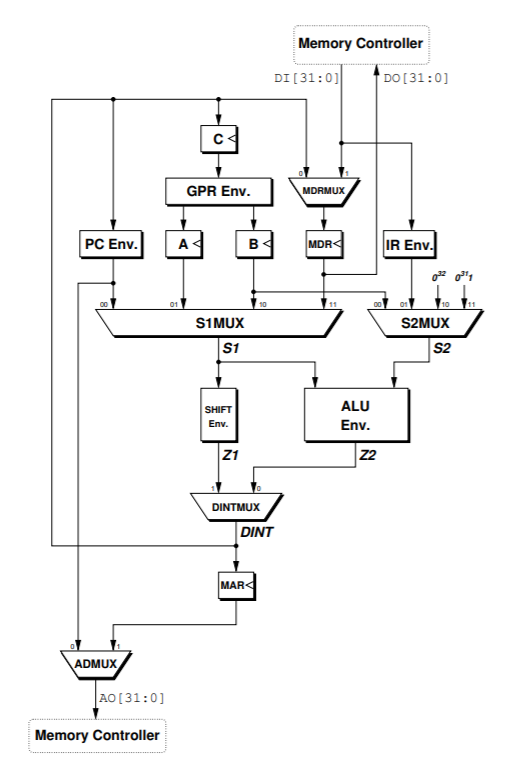
\includegraphics{Datapath.png}
    \caption{Datapath}
    \label{datapath}
  \end{figure}
\end{definition}

\begin{remark}
  The IR env. and GPR env. are connected by the addresses ${\tt Aadr}[4:0],{\tt Badr}[4:0],{\tt Cadr}[4:0]$.
\end{remark}

\begin{definition}
  The DLX controller is $19$ state FSM with state diagram depicted below:
  \begin{figure}[H]
    \centering
    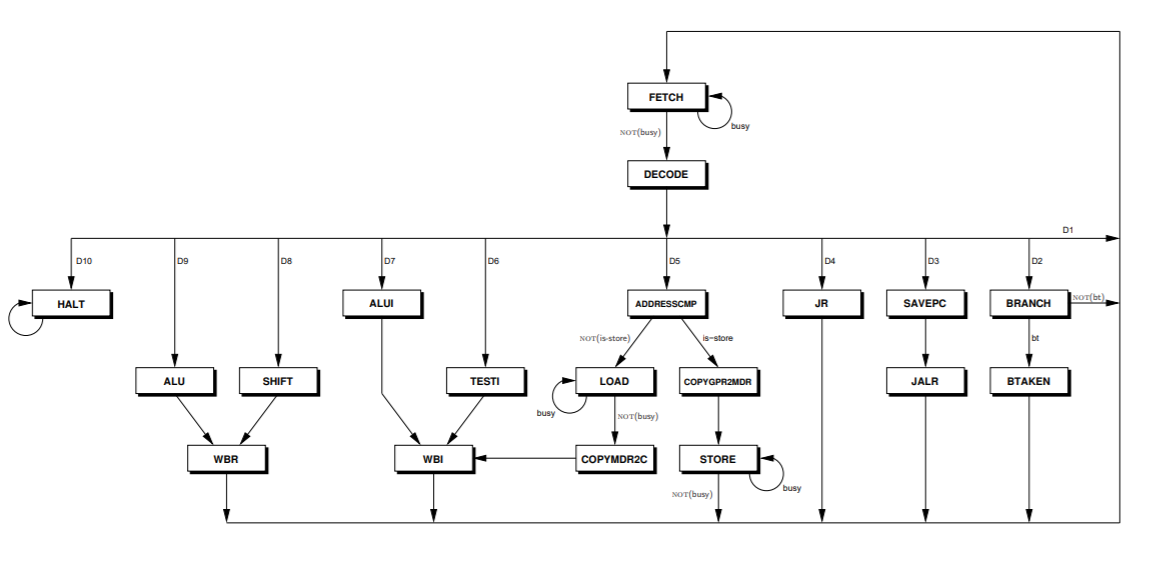
\includegraphics[width=\columnwidth]{DLXController.png}
    \caption{Controller}
    \label{controller}
  \end{figure}
  \noindent and here is a table with the RTL instructions (meaning Register Transfer Level) performed at each state. Each DLX instruction is broken down into a FETCH-DECODE-EXECUTE (which may contain many states) to perform it. Further, notice all executes, apart from HALT, DECODE, BRANCH, and instructions with busy flags, have $\degout = 1$. 
  \begin{table}[H]
    \centering
    \begin{tabular}{|c|p{4cm}|p{4cm}|}
      \hline
      State & RTL Instruction & Active Output \\\hline
      Fetch & $IR = M[PC]$ & ${\tt MR}, {\tt IRce}$ \\\hline
      Decode & A = RS1, B = RS2, PC=PC+1 & ${\tt Ace}$, ${\tt Bce}$, $S2sel[1]$, $S2sel[0]$, $add$, ${\tt PCce}$ \\\hline
      Alu & $C = A\text{ op }B$ & $S1sel[0]$, ${\tt Cce},$ some in $ALUF[2:0]$\\\hline
      TestI & $C = (A\text{ rel imm})$ & $S1sel[0]$, $S2sel[0]$, ${\tt Cce}$, $test$, ${\tt Itype},$ some in $ALUF[2:0]$ \\\hline
      AluI(add) & $C = A + imm$ & $S1sel[0]$, $S2sel[0]$, ${\tt Cce}$, $add$, ${\tt Itype}$ \\\hline
      Shift & $C = A\text{ shift }1$ & $S1sel[0]$, ${\tt Cce}$, $DINTsel$, $shift ,right$\\\hline
      Adr.Comp & $MAR = A + imm$ & $S1sel[0]$, $S2sel[0]$, ${\tt MARce}$, $add$ \\\hline
      Load & $MDR = M[MAR]$ & ${\tt MDRce}$, $ADsel$, ${\tt MR}$, $MDRsel$ \\\hline
      Store & $M[MAR] = MDR$ & $ADsel$, ${\tt MW}$ \\\hline
      CopyMDR2C & $C = MDR(>> 0)$ & $S1sel[0]$, $S1sel[1]$, $S2sel[1]$, $DINTsel$, ${\tt Cce}$ \\\hline
      CopyGPR2MDR & $MDR = B(<< 0)$ & $S1sel[1]$, $S2sel[1]$, $DINTsel$, ${\tt MDRce}$ \\\hline
      WBR & $RD = C $(R-type) & ${\tt GPR\_WE}$ \\\hline
      WBI & $RD = C $(I-type) & ${\tt GPR\_WE}$, ${\tt Itype}$\\\hline
      Branch & $bt={\tt AEQZ} \oplus {\tt Inst}[26]$ & \\\hline
      Btaken & $PC = PC + imm$ & $S2sel[0]$, $add$, ${\tt PCce}$ \\\hline
      JR & $PC = A$ & $S1sel[0]$, $S2sel[1]$, $add$, ${\tt PCce}$ \\\hline
      SavePC & $C = PC$ & $S2sel[1]$, $add$, ${\tt Cce}$ \\\hline
      JALR & $PC = A;\;R31 = C$ & $S1sel[0]$, $S2sel[1]$, $add$, ${\tt PCce}$, ${\tt GPR_WE}$, ${\tt JLINK}$ \\\hline
      HALT & & \\\hline
    \end{tabular}
  \end{table}
\end{definition}

\begin{thebibliography}{1}
  \bibitem[EvenMedina]{evenmedina} Guy Even and Moti Medina, "Digital Logic Design: A Rigorous Approach",  Cambridge University Press, 2019. Available online at \texttt{http://hyde.eng.tau.ac.il/Even-Medina/master.pdf}
  \bibitem[Even04]{even_cs} Guy Even, "Computer Structure; Spring 2004 Lecture Notes", manuscript, 2004. Available online at \texttt{http://hyde.eng.tau.ac.il/Computer\_Structure04/Notes/master.pdf}
  \bibitem[Even06]{even_ppcadder} Guy Even, "On teaching fast adder designs: revisiting Ladner \& Fischer"
  \bibitem[LadnerFischer]{ladnerfischer} R. Ladner and M. Fischer, "Parallel prefix computation", J. Assoc. Comput. Mach., 27, pp. 831–838, 1980.
\end{thebibliography}

\end{document}